\documentclass[11pt]{article}
\usepackage{amsmath,amssymb,amsthm,booktabs,graphicx,hyperref,enumitem,tikz,float}
\usepackage[margin=1in]{geometry}
\usepackage[export]{adjustbox}
\usepackage{caption}
\captionsetup{justification=raggedright,singlelinecheck=false,font=small}
\usetikzlibrary{calc,positioning,arrows.meta,decorations.pathreplacing,fit,backgrounds,shapes.symbols,shapes.geometric}

\usepackage[T1]{fontenc}
\usepackage{lmodern}
\usepackage{amssymb, amsmath, amsthm}
\usepackage{mathtools}
\usepackage[colorlinks=true, linkcolor=blue, citecolor=blue, urlcolor=blue]{hyperref}
\usepackage{lipsum}
\usepackage{comment}
\usepackage{enumitem}
\usepackage{tikz-cd}
\usepackage{tikz}
\usetikzlibrary{shapes,arrows,positioning,shadows}
\usepackage{xcolor}
\usepackage{algorithm}
\usepackage{algpseudocode}
\usepackage{caption}

\usepackage{verbatim}

\newenvironment{myalgorithm}[1][]{%
  \par\vspace{8pt}
  \noindent\hrule height.8pt
  \vspace{4pt}
  \ifblank{#1}{}{%
    \captionof{algorithm}{#1}%
    \vspace{4pt}
    \noindent\hrule height.4pt
    \vspace{6pt}
  }%
}{%
  \vspace{6pt}
  \noindent\hrule height.8pt
  \par\vspace{8pt}
}





% Custom packages
\usepackage{flexart}
% stylelibrary v2.3.1 (transparent box backgrounds by default: \opacityBack=0; see README.md).
\usepackage[many]{tcolorbox} %box environment
\usepackage[normalem]{ulem} %custom underline

% Bar width and spacing
\newlength{\framelinewidth}
\setlength{\framelinewidth}{0.6mm}
\newlength{\marginsep}
\setlength{\marginsep}{3pt}
\newlength{\defparindent}
\setlength{\defparindent}{15pt}
\setlength{\parindent}{\defparindent}
\newlength{\boxparskip}
\setlength{\boxparskip}{\parskip}

%Define colors
\definecolor{aicolor}{HTML}{038DFC}
\definecolor{editedaicolor}{HTML}{2B65C6}
\definecolor{humancolor}{HTML}{22AA22}
\definecolor{humanaicolor}{HTML}{5700FF}
\definecolor{defaultcolback}{HTML}{FFFFFF}  % white
\newcommand{\opacityFrame}{0.5} %Opacity Percentage for the Frame
\newcommand{\opacityText}{0.7} %Opacity Percentage for the Label Text
\newcommand{\opacityBack}{0} %Opacity Percentage for the Background (0 = fully transparent)

%Define footenote commands: Creates an aux file for the footnotes inside the boxes
\newif\iffootaux
\newcounter{footaux}% for \csname
\newcounter{auxpage}% to handle frontmatter etc.
\setcounter{auxpage}{1}

\makeatletter

\def\tcb@footnote@setup{
\let\footnotetext=\footaux
\let\footnote=\footnoteaux
}

\def\footnoteaux{\@ifnextchar[\@xfootnoteaux{\stepcounter{footnote}%
  \footnotemark[\thefootnote]\@footaux[\thefootnote]}}

\def\@xfootnoteaux[#1]{\footnotemark[#1]\@footaux[#1]}

\def\footaux{\@ifnextchar[\@footaux{\@footaux[\thefootnote]}}
\def\@footaux[#1]#2{\protected@write{\@auxout}{\let\theauxpage\relax}{\string\newfootnote{\theauxpage}{#1}{#2}}}

\newcommand{\newfootnote}[3]{% #1 = \theauxpage, #2 = \thefoontnote, #3 = text
  \ifnum#1=1\relax
    \footnotetext[#2]{#3}%
  \else
    \stepcounter{footaux}%
    \expandafter\xdef\csname footauxpage\thefootaux\endcsname{#1}%
    \expandafter\xdef\csname footauxnumber\thefootaux\endcsname{#2}%
    \expandafter\protected@xdef\csname footauxtext\thefootaux\endcsname{#3}%
  \fi}

% to run at the end of every page (debug version)
\newcommand{\addfootaux}{\loop
  \@ifundefined{footauxpage\thefootaux}{\footauxfalse}{%
    \count1=\csname footauxpage\thefootaux\endcsname\relax
    \advance\count1 by -1
    \ifnum\count1=\value{auxpage}%
      \expandafter\let\expandafter\footauxnumber\csname footauxnumber\thefootaux\endcsname
      \expandafter\let\expandafter\footauxtext\csname footauxtext\thefootaux\endcsname
      \footnotetext[\footauxnumber]{\footauxtext}%
      \footauxtrue
    \else
      \footauxfalse
    \fi}
  \iffootaux
    \global\expandafter\let\csname footauxpage\thefootaux\endcsname\relax
    \global\expandafter\let\csname footauxnumber\thefootaux\endcsname\relax
    \global\expandafter\let\csname footauxtext\thefootaux\endcsname\relax
    \stepcounter{footaux}%
  \repeat
\stepcounter{auxpage}}
\makeatother

\AtBeginDocument{\setcounter{footaux}{1}}% reset counter after \newfootnote
\AddToHook{shipout/after}{\addfootaux}


%Define box styles
\makeatletter
\tcbset{
    roundbox/.style={
    % Box Options
    rounded corners,
    arc=3mm,
    boxrule=\framelinewidth
  },
  rectanglebox/.style={
    % Box Options
    sharp corners,
    boxrule=\framelinewidth
  },
    linemargin/.style={
    % Box Options
    % Make frame with 1 line
    sharp corners,
    leftrule=\framelinewidth,    % Thickness of the left line
    rightrule=-0.1mm,            % Removes right frame
    toprule=-0.1mm,              % Removes top frame
    bottomrule=-0.125mm,         % Removes bottom frame
    % % make white background
    colback=white,
    opacityback=\opacityBack,
    % Oversize makes bigger, so that text alings with rest of the document
    oversize,
    % box margins
    left=\marginsep,
    right=\marginsep,
    top=0.5pt,
    bottom=0.5pt,
    before skip=0.5\baselineskip,
    after skip=0.5\baselineskip
  },
  alignoptions/.style={
    % box margins
    left=\marginsep,
    right=\marginsep,
    top=0.5pt,
    bottom=0.5pt,
    before skip=0.5\baselineskip,
    after skip=\parskip,
    before upper={
    \parindent=\defparindent
    \setlength{\parskip}{\boxparskip}
    }
  },
  %Format for footnotes to appear in the correct page
  footnoteformat/.style={
  before upper app=\tcb@footnote@setup
  }
}
\makeatother

\tcbset{
  enhancebreak/.style={
    % Box Options
    enhanced,
    breakable,
    skin first=enhanced,
    skin middle=enhanced,
    skin last=enhanced,
    % Oversize makes bigger, so that text alings with rest of the document
    oversize,
  },
}

% Label-to-bar separation (default 0.7pt; see README for usage).
% The overlay adds the fixed 2.65pt node-edge-to-glyph inset
% (default inner sep at \tiny) to this value for the node xshift.
\newcommand{\labelsepvalue}{0.7pt}
% `labeltopleft` (off) puts the label horizontally at the top-left
% corner, at the start of the block, instead of the rotated label.
\newif\iflabeltopleft
\tcbset{labeltopleft/.is if=labeltopleft}
% Per-box label text and color (set by each box env).
\newcommand{\boxlabeltext}{}
\newcommand{\boxlabelcolor}{black}
\tcbset{
  boxlabel/.store in=\boxlabeltext,
  boxlabelcolor/.store in=\boxlabelcolor,
  labeltopleftlayout/.code={%
    \iflabeltopleft \tcbset{top=12pt} \fi
  }
}
\tcbset{labelsep/.store in=\labelsepvalue}

% `extendbar` (on) extends the bar past the label glyphs by
% `barextend` (default 1pt); see README for usage. The floor is the
% label-node width + barextend − 7.19pt (calibrated node-to-glyph offset).
\newif\ifextendbar
\extendbartrue
\tcbset{extendbar/.is if=extendbar}
\newcommand{\barextendvalue}{1pt}
\tcbset{barextend/.store in=\barextendvalue}
\newcommand{\barextendoffset}{7.19pt}
\newsavebox{\extendbarbox}
\tcbset{
  extendbarmeasure/.code={%
    \iflabeltopleft\else
    \ifextendbar
      \sbox{\extendbarbox}{\tikz{\node[font=\tiny\bfseries\sffamily, align=right]{#1};}}%
      \tcbset{height=\dimexpr\wd\extendbarbox + \barextendvalue - \barextendoffset\relax, height plus=10000pt}%
    \fi
    \fi
  }
}

% Define Tcolorbox environments
%% Args: #1 additional options, #2 color, #3 Side text label
\newtcolorbox{labeledblock}[3][]{
    colframe=#2,opacityframe=\opacityFrame,
    enhancebreak, alignoptions, linemargin,
    colback=white,
    frame hidden,
    borderline west={\framelinewidth}{0pt}{#2, opacity=\opacityFrame},
    overlay={
    \iflabeltopleft
    \node[anchor=north west, inner sep=0pt, font=\scriptsize\bfseries\sffamily, text=\boxlabelcolor, text opacity=\opacityText] at ([xshift=7.5pt, yshift=-2pt]frame.north west) {\boxlabeltext};
    \else
    \node[
    #2, font=\tiny\bfseries\sffamily,
    rotate=90, anchor=south east, align=right,
    text opacity=\opacityText
      ]
      at ([xshift=2.65pt-\labelsepvalue, yshift=3.8pt]frame.north west) {#3};
    \fi
    }, footnoteformat,
    boxlabel={#3}, boxlabelcolor=#2,
    #1,
    labeltopleftlayout, extendbarmeasure={#3}
}

\newtcolorbox{humanblock}[1][]{
    colframe=humancolor, opacityframe=\opacityFrame,
    enhancebreak, alignoptions, linemargin,
    colback=white,
    frame hidden,
    borderline west={\framelinewidth}{0pt}{humancolor, opacity=\opacityFrame},
    overlay={
    \iflabeltopleft
    \node[anchor=north west, inner sep=0pt, font=\scriptsize\bfseries\sffamily, text=\boxlabelcolor, text opacity=\opacityText] at ([xshift=7.5pt, yshift=-2pt]frame.north west) {\boxlabeltext};
    \else
    \node[
    humancolor, font=\tiny\bfseries\sffamily,
    rotate=90, anchor=south east, align=right,
    text opacity=\opacityText
      ]
      at ([xshift=2.65pt-\labelsepvalue, yshift=3.8pt]frame.north west) {Human};
    \fi
    }, footnoteformat,
    boxlabel=Human, boxlabelcolor=humancolor,
    #1,
    labeltopleftlayout, extendbarmeasure={Human}
}

\newtcolorbox{humanaiblock}[1][]{
    colframe=humanaicolor, opacityframe=\opacityFrame,
    enhancebreak, alignoptions, linemargin,
    colback=white,
    frame hidden,
    borderline west={\framelinewidth}{0pt}{humanaicolor, opacity=\opacityFrame},
    overlay={
    \iflabeltopleft
    \node[anchor=north west, inner sep=0pt, font=\scriptsize\bfseries\sffamily, text=\boxlabelcolor, text opacity=\opacityText] at ([xshift=7.5pt, yshift=-2pt]frame.north west) {\boxlabeltext};
    \else
    \node[humanaicolor, font=\tiny\bfseries\sffamily, rotate=90, anchor=south east, align=right,
      text opacity=\opacityText
      ]
      at ([
      xshift=2.65pt-\labelsepvalue, yshift=3.8pt
      ]frame.north west) {Human + AI};
    \fi
    }, footnoteformat,
    boxlabel={Human + AI}, boxlabelcolor=humanaicolor,
    #1,
    labeltopleftlayout, extendbarmeasure={Human + AI}
}

\newtcolorbox{aiblock}[1][]{
    colframe=aicolor, opacityframe=\opacityFrame,
    enhancebreak, alignoptions, linemargin,
    colback=white,
    frame hidden,
    borderline west={\framelinewidth}{0pt}{aicolor, opacity=\opacityFrame},
    overlay={
    \iflabeltopleft
    \node[anchor=north west, inner sep=0pt, font=\scriptsize\bfseries\sffamily, text=\boxlabelcolor, text opacity=\opacityText] at ([xshift=7.5pt, yshift=-2pt]frame.north west) {\boxlabeltext};
    \else
    \node[aicolor, font=\tiny\bfseries\sffamily, rotate=90, anchor=south east, align=right,
      text opacity=\opacityText
      ]
      at ([xshift=2.65pt-\labelsepvalue, yshift=3.8pt]frame.north west) {AI};
    \fi
    }, footnoteformat,
    boxlabel=AI, boxlabelcolor=aicolor,
    #1,
    labeltopleftlayout, extendbarmeasure={AI}
}

\newtcolorbox{editedaiblock}[1][]{
    colframe=editedaicolor, opacityframe=\opacityFrame,
    enhancebreak, alignoptions, linemargin,
    colback=white,
    frame hidden,
    borderline west={\framelinewidth}{0pt}{editedaicolor, opacity=\opacityFrame},
    overlay={
    \iflabeltopleft
    \node[anchor=north west, inner sep=0pt, font=\scriptsize\bfseries\sffamily, text=\boxlabelcolor, text opacity=\opacityText] at ([xshift=7.5pt, yshift=-2pt]frame.north west) {\boxlabeltext};
    \else
    \node[editedaicolor, font=\tiny\bfseries\sffamily, rotate=90, anchor=south east, align=right,
      text opacity=\opacityText
      ]
      at ([
      xshift=2.65pt-\labelsepvalue, yshift=3.8pt]frame.north west) {Edited AI};
    \fi
    }, footnoteformat,
    boxlabel={Edited AI}, boxlabelcolor=editedaicolor,
    #1,
    labeltopleftlayout, extendbarmeasure={Edited AI}
}


%%%---------------------- Underline Commands -------------------------

% Dash pattern:
\gdef\dashpattern{\kern.05em\lower.3ex\vbox{\hrule width.2em\kern.1ex}}

\def\humanul{\textcolor{humancolor}\bgroup\markoverwith{\kern.05em\lower.3ex\vbox{\hrule width.2em\kern.1ex}\kern.05em}\ULon}

\def\aiul{\textcolor{aicolor}\bgroup\markoverwith{\kern.05em\lower.3ex\vbox{\hrule width.2em\kern.1ex}\kern.05em}\ULon}

%%% Macros
%%%_____________________________________

\newcommand{\Muse}{\footnotesize with {Muse Spark} via {\ttfamily \href{http://meta.ai}{meta.ai}}}
\newcommand{\HumanLabel}{
({\bfseries\sffamily\color{humancolor!70}Human})
}
\newcommand{\AILabel}{
({\bfseries\sffamily\color{aicolor!70}AI})
}
\newcommand{\HumanAILabel}{
({\bfseries\sffamily\color{humanaicolor!70}Human + AI})
}
\newcommand{\EditedAILabel}{
({\bfseries\sffamily\color{editedaicolor!70}Edited AI})
}
\newcommand{\AIAssistedLabel}{
({\bfseries\sffamily\color{aiassistedcolor!70}AI-assisted})
}
\newcommand{\OtherLabel}{
({\bfseries\sffamily\color{othercolor!70}Other})
}


%GAP Code boxes
\definecolor{codebg}{RGB}{245,245,245}
\usepackage{listings}
%
\lstdefinelanguage{GAP}{
  morekeywords={if,then,else,elif,fi,for,do,od,while,local,function,return,rec,Error},
  sensitive=true,
  morecomment=[l]{\#},
  morestring=[b]",
  morestring=[b]'
}
\lstset{
  language=GAP,
  basicstyle=\footnotesize\ttfamily,
  keywordstyle=\color{blue}\bfseries, % <- blue differentiators
  commentstyle=\color{gray}\itshape,
  stringstyle=\color{red!60!black},
  backgroundcolor=\color{codebg},
  frame=single,
  framerule=0.4pt,
  rulecolor=\color{black!5},
  breaklines=true,
  columns=fullflexible,
  keepspaces=true,
  upquote=true,
  showstringspaces=false
}

% Python code listings: read from the ancillary .py file rather than pasted inline. The
% scripts live in this repository's Formalization/Appendix_* folders.
\newcommand{\ancillary}[1]{../../Formalization/#1}
\lstdefinestyle{pycode}{
  language=Python,
  basicstyle=\scriptsize\ttfamily,
  keywordstyle=\color{blue}\bfseries,
  commentstyle=\color{gray}\itshape,
  stringstyle=\color{red!60!black},
  backgroundcolor=\color{codebg},
  frame=single,
  framerule=0.4pt,
  rulecolor=\color{black!5},
  breaklines=true,
  breakatwhitespace=false,
  columns=fullflexible,
  keepspaces=true,
  tabsize=4,
  upquote=true,
  showstringspaces=false,
  numbers=left,
  numberstyle=\tiny\color{black!40},
  xleftmargin=2em,
  extendedchars=true,
  literate={—}{{---}}1 {–}{{--}}1 {‘}{{`}}1 {’}{{'}}1
}

\theoremstyle{plain}
\newtheorem{theorem}{Theorem}[section]
\newtheorem{lemma}[theorem]{Lemma}
\newtheorem{corollary}[theorem]{Corollary}
\newtheorem{proposition}[theorem]{Proposition}
\newtheorem{conjecture}[theorem]{Conjecture}
\theoremstyle{definition}
\newtheorem{definition}[theorem]{Definition}
\newtheorem{example}[theorem]{Example}
\newtheorem{remark}[theorem]{Remark}
\newtheorem{question}[theorem]{Question}

\title{Accidental Cancellations in Cholesky Factorization}
\primaryauthors{{\scshape Nam Trang} \\ \Muse}

\secondaryauthors{{\scshape Paul Bendich} \and {\scshape Patrick Tam}}

\subjclass[2020]{65F50; 15A23, 05C50, 15B48, 05C75, 62H22}

\flexabstract{
Sparse Cholesky factorization allocates storage from the symbolic fill pattern $G^+$ alone, assuming that no position predicted nonzero ever cancels. Over-allocation never threatens correctness, so the assumption is safe in practice, but it leaves open an existential question, recorded by the first author in unpublished notes circulated in 2021 as two conjectures. Call an ordering $\sigma$ clean for an SPD matrix $A$ if every position predicted nonzero in $G^+_\sigma$ is nonzero in the factor $L$. Conjecture~1: every irreducible SPD matrix admits a clean ordering. Conjecture~2: every irreducible SPD matrix admits an ordering whose first Schur complement has no cancellation at a predicted-nonzero position.

We refute both. Conjecture~1 fails at every even order $n\ge6$, via an explicit family $M_{2m}$ on the complete graph. The family is not exhibited but derived: classifying the zero-configurations available at a level with four surviving vertices forces a fixed-point-free involution --- hence even order --- forces the magnitudes $AB$ within pairs and blocks $[[A,B],[B,A]]$ across them, and forces the parameters onto the measure-zero curve $A^2+(1-B^2)A-1=0$. Conversely every point of that curve with $0<B<1$ yields a counterexample at every even order $n\ge6$, so the construction is a one-parameter family rather than a single matrix. Conjecture~2 already fails at order~$4$, via $A^*$ with spectrum $\{9,3,3,1\}$: none of its $24$ orderings has a cancellation-free first Schur complement, yet $8$ of them give a clean factor --- the refill phenomenon that separates the two conjectures, and the trap that invalidates any argument conflating Schur-complement zeros with factor zeros.

Positively, Conjecture~1 holds for every irreducible SPD matrix of order at most~$4$, by an elementary argument; order five we leave open, and we settle no further order exhaustively. At order six the complete graph $K_6$ fails, by the family above. Forests are clean in the strong form that every ordering is clean --- recovering, in factorization language, a covariance-faithfulness theorem of Malouche and Rajaratnam --- and so are $2$-path strips and dominating-vertex fans, chordal graphs with exactly one triangle, and chordal graphs of clique number at most $3$ with pairwise edge-disjoint triangles; on the last four classes the clean ordering must adapt to the matrix, since no fixed ordering suffices. Odd orders $n\ge7$ remain open, and we explain why the pairing argument that settles the even orders
does not extend to them.
}


\begin{document}
\maketitle



%\tableofcontents

    

\section{Introduction}
\begin{humanblock}
\subsection{Sparse Cholesky and the price of fill}

Let $A$ be a real symmetric positive definite matrix of order $n$. Its Cholesky factorization $A = LL^\top$ is the workhorse of direct methods for the linear systems arising in finite-element analysis, interior-point methods, Gaussian process regression, and maximum-likelihood estimation in graphical models. When $A$ is sparse, the cost of the factorization is governed not by $n$ but by the number of nonzeros in $L$, and that number depends on the order in which variables are eliminated. Eliminating a variable makes its surviving neighbors mutually adjacent, so positions that were structurally zero in $A$ may become nonzero in $L$. These are the fill entries, and controlling them is the central problem of sparse direct methods.

The combinatorial description is due to Rose, Tarjan and Lueker \cite{Rose}. Represent the sparsity of $A$ by its pattern graph $G_A$, with an edge $\{i,j\}$ whenever $A_{ij} \neq 0$. For an ordering (or permutation) $\sigma$ of $\{0,1,\dots,n-1\}$, play the elimination game: repeatedly delete the next vertex (in the ordering given by $\sigma$) and complete its neighborhood into a clique. The resulting graph $G^+_\sigma$ contains every position that can be nonzero in $L$, and the fill-path theorem characterizes it exactly: $\{j,k\}$ is an edge of $G^+_\sigma$ precisely when $G_A$ contains a $j$--$k$ path all of whose interior vertices precede both endpoints. Choosing $\sigma$ to minimize fill is NP-hard \cite{Yannakakis}, which is why practical codes rely on heuristics and on the elimination-tree machinery surveyed by Heath, Ng and Peyton \cite{Heath} and Davis \cite{Davis}.

\subsection{The no-cancellation assumption}

Every sparse Cholesky implementation performs a symbolic factorization before touching a single floating-point number: it computes $G^+_\sigma$ from $G_A$ alone and allocates exactly that much storage. This step is purely graph-theoretic, and it is where an assumption enters. The code takes for granted that a position predicted nonzero is nonzero -- that once an entry fills in, it never cancels back to zero. Demmel's lecture notes state it without apology: ``assume that there is no cancellation, i.e. that once an entry of $A$ gets filled in, it never cancels out later (which would be highly unlikely anyway)'' \cite{Demmel}.

The assumption is harmless for its intended purpose, and it is worth being precise about why. Symbolic factorization produces an upper bound on the structure of $L$. If a predicted nonzero happens to cancel, the code has reserved a slot it does not need: it over-allocates slightly and computes the correct answer. Cancellation is a performance question, never a correctness question. Nor is the parenthetical wrong: a cancellation requires an exact algebraic coincidence among the entries of $A$, and such coincidences form a set of Lebesgue measure zero.

So the practice is sound and the heuristic is true. But both are statements about a fixed ordering and about typical matrices, and neither answers the question a mathematician would ask next.

In sum, the results in this paper do not contradict expert expectations, they live on its complement. Experts expected the generic statement, and it holds; the conjectures are existential and quantify over all SPD matrices, including the measure-zero locus where the counterexamples lie. 

\subsection{The existential question}\label{sec:intro-exist}

Fix a matrix, not an ordering, and ask whether some ordering is free of cancellation. Call $\sigma$ clean for $A$ if for every edge $\{j,k\}\in G^+_\sigma$, letting $S$ be the set of vertices preceding $\min(\sigma^{-1}(j),\sigma^{-1}(k))$ in $\sigma$, we have $(A/A_S)_{jk}\neq0$ — i.e. the entry is nonzero at the stage where the earlier of $j,k$ is pivoted, so the predicted nonzero is realized in $L$. This is the factor definition, not the Schur-complement definition requiring $(A/A_S)_{jk}\neq0$ for every stage $S$ whenever $\{j,k\}\in G_S$; the latter conflates Schur zeros with factor cancellations and would give $A^*$ no clean ordering at all, unlike the eight of Theorem~\ref{thm:Astar}, because it ignores the refill phenomenon. Two conjectures, recorded by Trang in unpublished notes in 2021, ask:
\newline

\noindent \textbf{Conjecture~1.} Every irreducible SPD matrix admits a clean ordering.
\newline

\noindent \textbf{Conjecture~2.} Every irreducible SPD matrix admits an ordering whose first Schur complement has no cancellation at a predicted-nonzero position.
\newline

These are genuinely different from the implementation's assumption, in two ways. First, they are existential: they permit the ordering to depend on the numerical entries of $A$, whereas symbolic factorization must choose $\sigma$ from $G_A$ alone. Second, they quantify over all SPD matrices, including the measure-zero ones the genericity heuristic sets aside. A counterexample must therefore be an exact algebraic object, and this is exactly why ``cancellation is unlikely'' and ``Conjecture~1 is false'' can both be true: the two statements live on complementary sets.

Conjecture~2 is the stronger demand, and the gap between them is the phenomenon we call refill. A zero created in one Schur complement is not yet a cancellation in $L$: the entry $(j,k)$ is committed only when the earlier of $j,k$ is pivoted, and an intervening elimination can restore it to a nonzero value. Any analysis that conflates Schur-complement zeros with factor zeros will reach false conclusions.%, and several arguments corrected in this paper did exactly that.

\subsection{The same question in statistics}\label{sec:stats}

The existential question has a second life in Gaussian graphical models, where a zero in a Schur complement is a conditional independence: $(A/A_S)_{jk} = 0$ says exactly that $X_j$ and $X_k$ are conditionally independent given $X_S$. A distribution is faithful to its graph when no conditional independence holds beyond those the graph implies, so a cancellation at a predicted-nonzero position is a failure of faithfulness.

That literature has settled one case decisively. Malouche and Rajaratnam \cite{Malouche} proved, using the covariance--precision path formula of Jones and West \cite{Jones}, that a Gaussian whose covariance graph is a tree is necessarily covariance faithful. The dual statement for concentration graphs is older still: Becker, Geiger and Meek~\cite{Becker} proved that a Gaussian whose concentration graph is a tree is necessarily concentration faithful. In our language the covariance version is Conjecture~1 for forests, in the strong form that every ordering is clean -- proved fifteen years ago under a different name, its dual a decade earlier again, and neither cited in the numerical literature that assumes it. Beyond trees the two communities part company: Meek \cite{Meek} and Uhler, Raskutti, B\"uhlmann and Yu \cite{Uhler} study when faithfulness holds generically, showing that unfaithful distributions have measure zero while strong-faithfulness failures occupy a set of positive measure, but neither literature asks whether some ordering can always be chosen to avoid the failures that do occur.

\subsection{Results}

We answer the existential question negatively in general and positively on a substantial and now precisely delimited class.

Conjecture~2 is false at order~4 (Theorem~\ref{thm:Astar}): an explicit matrix $A^*$ with spectrum $\{9,3,3,1\}$ has no ordering whose first Schur complement is cancellation-free, although $8$ of its $24$ orderings give a clean factor -- the refill phenomenon in its simplest form.

Conjecture~1 holds for $n\le4$ by an elementary case analysis of the six connected patterns on four vertices, with no computation (Theorem~\ref{thm:leq4}), and is false at every even order at least~6 (Theorem~\ref{thm:M2m}), via a family $M_{2m}$ built from a pairing of the vertices, with within-pair entries of magnitude $AB$ and cross-pair blocks $[[A,B],[B,A]]$. The family is not exhibited but derived: at any level with four surviving vertices, exactly three of the $4096=2^{12}$ candidate zero-configurations are feasible and use all four vertices as pivots, and each is a fixed-point-free involution (Lemma~\ref{lem:pairing}). The three magnitudes and the block structure are forced as the unique solution of the resulting additive system; the requirement of a fixed-point-free involution is precisely why the order must be even. The parameters are forced onto the measure-zero curve $A^2+(1-B^2)A-1=0$, and conversely every point of that curve with $0<B<1$ yields a counterexample (Remark~\ref{rem:curve-family}), so the construction is a one-parameter family; the instance $B=1/2$, with $A=(-3+\sqrt{73})/8$, is the one we verify explicitly.

Order~5 remains open (Section~\ref{sec:status}). At order six the complete graph $K_6$ fails, by Theorem~\ref{thm:M2m}; the other connected patterns of order six, the $14$-edge pattern $K_6-e$ among them, remain open.

Structural classes. Independently of the order-by-order picture we prove Conjecture~1 for forests in the strong form above; for 2-path strips and dominating-vertex fans; for chordal graphs with exactly one triangle; and for chordal graphs of clique number at most $3$ whose triangles are pairwise edge-disjoint. Beyond forests the clean ordering must adapt to the matrix: the triangle lies in each of these classes, and no fixed ordering is clean for every SPD matrix whose pattern is a triangle (Remark~\ref{rem:no-fixed}).

  The counterexamples refuting both conjectures, and the structural classes of Section \ref{sec:positive} beyond forests, were found with AI assistance and insight; AI finds the counterexamples in Section \ref{sec:even}, provides the calculations showing the counterexamples work, and comes up with key ideas for the proofs in Section \ref{sec:positive}. 

Odd orders at least~7 remain open. The reason is structural rather than computational: the
classification of Lemma~\ref{lem:pairing} that forces the even construction requires exactly four
surviving vertices, and its injectivity step fails at five, so parity confers no protection at odd
orders. Remark~\ref{rem:even-needed} records this together with the two computations that delimit the
position --- no scheme leaving one survivor at every vertex exists at order five, and an exhaustive
search at order seven did not terminate.

\subsection{Method}

Three devices carry the analysis. We recast cleanliness as a covering problem: a slot $(S, \{j,k\})$ asserts $(A/A_S)_{jk} = 0$, and Conjecture~1 fails exactly when some blocking family of slots -- one hitting every ordering -- is realizable by an SPD matrix. Second, since a cancellation reads $r_{jk} = r_{uj}r_{uk}$, the substitution $t^{(S)}_{jk} = -\log|r^{(S)}_{jk}|$ makes every cancellation additive, $t^{(S)}_{jk} = t^{(S)}_{uj} + t^{(S)}_{uk}$, with $t^{(S)}_{jk}>0$ forced by strict definiteness; obstructions then become statements about a linear system, refutable by Stiemke's lemma \cite{Stiemke,Gordan} with exact rational certificates. Third, unrealizability is monotone in the slot family (Lemma~\ref{lem:monotone}), which is what makes exhaustive search over patterns finite and sound.

\subsection{Related work}

Four strands of literature bear on the existential question, and it is worth saying what we take from
each.

\emph{Sparse direct methods.} The combinatorial model is due to Rose, Tarjan and Lueker~\cite{Rose}:
the elimination game, the fill graph $G^+_\sigma$, and the fill-path theorem characterizing its edges
by paths whose interior has already been eliminated. Everything symbolic in this paper is a
consequence of that characterization, recorded here as Proposition~\ref{prop:fillpath}; what we add is
the question of when the symbolic prediction is numerically exact. Minimizing fill is
NP-hard~\cite{Yannakakis}, which is why production codes choose the ordering by heuristics, and the
accounts of Heath, Ng and Peyton~\cite{Heath} and of Davis~\cite{Davis} describe the two-phase
practice that Section~\ref{sec:practical} addresses: a symbolic phase allocates for $G^+_\sigma$, and
a numeric phase fills that structure in. Demmel's lecture notes~\cite{Demmel} state the underlying
assumption explicitly. Our results separate two readings of it: as an allocation bound it is correct,
since the numeric pattern is always contained in the symbolic one (Definition~\ref{def:numeric}), but
as an existential statement about orderings it is false at every even order from six onwards.

\emph{Chordal graphs.} The positive results of Section~\ref{sec:positive} proceed by choosing
simplicial pivots, so they rest on the classical theory: Dirac's theorem that a chordal graph has a
simplicial vertex~\cite{Dirac}, the characterization of chordality by perfect elimination
orderings~\cite{Fulkerson}, and the standard treatment of Golumbic~\cite{Golumbic}. Our setting
differs from the usual one in a way worth emphasizing. A perfect elimination ordering is optimal for
fill, but optimality for fill is not cleanliness: Remark~\ref{rem:peo-fail} exhibits a $2$-path strip
and SPD realizations of it for which no fill-free ordering is clean, so the induction of
Theorem~\ref{thm:positives} must sometimes create fill deliberately. The strip and fan classes are
partial $2$-trees in the sense of Bodlaender~\cite{Bodlaender}, and general partial $2$-trees are the
natural next case, which is why they head the list of open problems in Section~\ref{sec:status}.

\emph{Gaussian graphical models and faithfulness.} Under the dictionary of Lauritzen~\cite{Lauritzen},
a Schur-complement zero is a conditional independence, so a cancellation at a predicted-nonzero
position is a failure of faithfulness. Malouche and Rajaratnam~\cite{Malouche} proved that a Gaussian
whose covariance graph is a tree is covariance faithful; in our language that is the Fill-Graph
Conjecture for forests in the strong form that every ordering is clean, and
Theorem~\ref{thm:forest} re-derives it in factorization language using the path formula of Jones and
West~\cite{Jones}, which is also the identity that drives the proof. Trek
separation~\cite{Sullivant} gives the general combinatorial criterion for vanishing minors in such
models, and our slots are instances of the vanishing conditions it classifies. The faithfulness
literature then parts company with our question, and the difference is worth stating precisely:
Meek~\cite{Meek}, Zhang and Spirtes~\cite{Zhang}, and Uhler, Raskutti, B\"uhlmann and Yu~\cite{Uhler}
ask when faithfulness holds \emph{generically} or \emph{strongly}, and show that unfaithful
distributions form a set of measure zero while strong-faithfulness failures occupy a set of positive
measure. Those are statements about typical matrices. Ours is existential and quantifies over all SPD
matrices, so a counterexample must be an exact algebraic object and necessarily lives on the
measure-zero locus that this literature sets aside; Appendix~\ref{app:recheck} explains how the two
coexist.

\emph{Tools.} Three further bodies of work are used technically rather than thematically. The quotient
identity for Schur complements, which is what licenses treating a level as a set rather than a
sequence, is due to Haynsworth and to Crabtree and Haynsworth~\cite{Haynsworth,Crabtree}; it appears
here as Lemma~\ref{lem:quotient}. Which zero patterns are realizable by an SPD matrix at all is the
positive-definite completion problem of Grone, Johnson, S\'a and Wolkowicz~\cite{Grone}, with clique
trees~\cite{Blair} as the structure behind the chordal case; this is the background against which our
notion of realizability should be read, since a blocking family refutes the conjecture only if some
SPD matrix realizes it. The conditional-independence axioms for Gaussians catalogued by Lnenicka and
Matus~\cite{Lnenicka} contain our Nesting Lemma~\ref{lem:nesting} as the weak-transitivity axiom.
Finally, the infeasibility certificates of Section~\ref{sec:core} are an application of Stiemke's
transposition theorem~\cite{Stiemke}, a refinement of Gordan's~\cite{Gordan}.

\subsection{Organization}

Section~\ref{sec:setting} sets notation and states conjectures. Section~\ref{sec:core} proves core lemmas. Section~\ref{sec:positive} proves positive results including PEO-insufficiency witness. Section~\ref{sec:even} proves Pairing Lemma, derives $M_{2m}$, and states $A^*$. Section~\ref{sec:status} states open problems and established results. Appendix gives computational protocol. Figures illustrate the forest path formula, the refill mechanism, the strip induction, and the pairing structure of $M_{2m}$.

\subsection{Why it matters}\label{sec:why}
These results close a foundational gap between theory and practice felt in several communities. For numerical linear algebra and sparse direct solvers, symbolic factorization allocates $G^+$ from the graph alone assuming no cancellation; we show the assumption is safe for correctness (over-allocation) yet false existentially: $G^L_\sigma=G^+_\sigma$ cannot be guaranteed for all SPD matrices, the smallest known failure occurring at order $6$ ($K_6$, via $M_6$; order five is open). Order $4$ already obstructs the weaker first-Schur version ($A^*$: $0/24$ stage-$1$ clean), while its $8/24$ clean factors show that refill separates the two questions.

For graph theory and combinatorial matrix theory, we map the boundary of when a chordal completion can be realized without algebraic accident: forests are strongly clean (every ordering clean), $2$-path strips, fans, one-triangle adaptive, and edge-disjoint triangles with $\omega\le3$ are clean, while $K_6$ fails. Beyond order four, every positive class has clique number at most $3$, while the failures we construct are complete graphs; the $4$-vertex pairing involution forced on the curve $A^2+(1-B^2)A-1=0$ explains how these fail, and where the boundary lies in between is open.

For statistics, graphical models, and causal inference, a cancellation $(A/A_S)_{jk}=0$ is a failure of faithfulness. We re-derive, in factorization language, Malouche and Rajaratnam's result that forests are faithful in the strong form every ordering clean (proved under a different name fifteen years ago, never cited in the numerical literature that assumes it). We exhibit measure-zero unfaithful $M_{2m}$ on $K_{2m}$ with $A^2+(1-B^2)A-1=0$, and explain why unfaithfulness has measure zero (faithfulness is generic) yet coexists with existential failure.

For theoretical computer science, the covering problem over slots and the integer Stiemke certificates $y^\top T\ge0$ used to refute blocking families provide a transposition-theorem view of when a chordal completion can be realized without algebraic accident.
\end{humanblock}



\section*{Statement of AI Use}

\begin{humanblock}
This paper was developed through collaboration between researchers and Muse Spark (AI model) via the \href{http://meta.ai}{meta.ai} chat interface. The model helped explore ideas, develop candidate arguments, and draft material. Researchers guided the work, checked and corrected the mathematics, and take ownership for the final manuscript. Following \cite{schmitt2025extremal}, margin markers identify human-drafted \!\!\HumanLabel and AI-assisted material \!\!\AILabel separately.
\end{humanblock}

\section*{Concurrent Work}
\begin{humanblock}
We are not aware of any concurrent work at the time of publication.
\end{humanblock}



\section{Setting, vocabulary, and conjectures}\label{sec:setting}
\begin{humanblock}
This section fixes every notion used in Sections~\ref{sec:core}--\ref{sec:even}. It is meant to be
read once and consulted thereafter; Table~\ref{tab:notation} collects the notation. Three points are
worth flagging before the formal definitions. First, we work with two graphs at once: a
\emph{symbolic} graph predicted from the sparsity pattern alone, and the \emph{numeric} pattern of
the actual Schur complement. The whole subject is the gap between them. Second, elimination is
indexed by \emph{sets} rather than sequences, which is legitimate by the quotient property
(Lemma~\ref{lem:quotient}). Third, a \emph{slot} is a formal assertion that some entry vanishes; it
becomes true or false only relative to a matrix, and that distinction drives the entire method.

\subsection{SPD matrices and Schur complements of sets}

\begin{definition}[SPD]\label{def:spd}
A symmetric $n\times n$ real matrix $A$ is \emph{symmetric positive definite} (SPD), written
$A\succ0$, if $x^\top Ax>0$ for every $x\neq0$. Throughout, $V=\{0,1,\dots,n-1\}$ indexes the rows
and columns of $A$, and we freely call the elements of $V$ \emph{vertices}.
\end{definition}

\begin{definition}[Schur complement of a set]\label{def:spd-schur}
Let $A$ be symmetric and let $S\subseteq V$ be \emph{any} subset with $A_{SS}\succ0$; put
$R=V\setminus S$ and write $A=\begin{pmatrix}A_{SS}&A_{SR}\\A_{RS}&A_{RR}\end{pmatrix}$ after a
symmetric permutation. The \emph{Schur complement of $S$ in $A$} is the matrix on $R$
\[
A/A_S = A_{RR}-A_{RS}(A_{SS})^{-1}A_{SR}.
\]
For a single vertex, $A/A_{\{v\}}=B-rr^\top/a$ when $A=\begin{pmatrix}a&r^\top\\r&B\end{pmatrix}$ with
$a=A_{vv}$. For an ordering $\sigma=(v_1,\dots,v_n)$ we abbreviate $S^{(0)}=A$ and
$S^{(j)}=A/A_{\{v_1,\dots,v_j\}}$.
\end{definition}

\begin{proposition}[Basic properties]\label{prop:schur-basic}
If $A\succ0$ and $S\subseteq V$ then $A_{SS}\succ0$, so $A/A_S$ is defined, and $A/A_S\succ0$.
Moreover $A/A_S$ depends only on the \emph{set} $S$, not on any ordering of it.
\end{proposition}
\begin{proof}
$A_{SS}\succ0$ because it is a principal submatrix of $A$. For $y$ supported on $R$, one has
$y^\top(A/A_S)y=\min\{x^\top Ax : x|_R=y\}>0$, so $A/A_S\succ0$. Order-independence is immediate from
the closed formula of Definition~\ref{def:spd-schur}, which mentions no ordering of $S$; the
compatibility with step-by-step elimination is Lemma~\ref{lem:quotient}.
\end{proof}

\begin{lemma}[Quotient property, transitivity of Schur complements]\label{lem:quotient}
Let $A\succ0$, $S\subset V$ and $v\in V\setminus S$, and set $M=A/A_S$. Then
\[
M/M_{\{v\}} = A/A_{S\cup\{v\}}
\]
as matrices on $V\setminus(S\cup\{v\})$. That is, eliminating $S$ and then $v$ gives the same result
as eliminating $S\cup\{v\}$ at once.
\end{lemma}
\begin{proof}
Write $A$ partitioned, with $R=V\setminus(S\cup\{v\})$, as
\[
A=\begin{pmatrix}A_{SS}&A_{Sv}&A_{SR}\\A_{vS}&a_{vv}&a_{vR}\\A_{RS}&a_{Rv}&A_{RR}\end{pmatrix}.
\]
Then $A/A_S=\begin{pmatrix}b&c\\c^\top&A_{RR}-A_{RS}A_{SS}^{-1}A_{SR}\end{pmatrix}$ where
$b=a_{vv}-A_{vS}A_{SS}^{-1}A_{Sv}$ and $c=a_{vR}-A_{vS}A_{SS}^{-1}A_{SR}$. Taking the Schur
complement of $\{v\}$ in $M$ yields $A_{RR}-A_{RS}A_{SS}^{-1}A_{SR}-cb^{-1}c^\top$, which is
$A/A_{S\cup\{v\}}$ by block inversion of $A_{S\cup\{v\},S\cup\{v\}}$. See Haynsworth
\cite{Haynsworth} and Crabtree--Haynsworth \cite{Crabtree} for the general quotient formula.
\end{proof}

\begin{remark}[Levels and stages]\label{rem:level-stage}
Because of Proposition~\ref{prop:schur-basic} and Lemma~\ref{lem:quotient} we may speak of a
\emph{level}: a set $S\subseteq V$ of already-eliminated vertices, with $A/A_S$ the matrix currently
being factored and $R=V\setminus S$ the \emph{survivors}. The \emph{stage} is the number $|S|$ of
completed eliminations, so an ordering passes through levels
$\emptyset=S_0\subset S_1\subset\cdots\subset S_n=V$ with $|S_j|=j$. ``Level'' is thus a set and
``stage'' is a counter; a statement ``at level $S$'' is a statement about the single matrix $A/A_S$,
whereas a statement ``at stage $j$'' refers to whichever level of size $j$ the ordering has reached.
\end{remark}

\subsection{Pivots, the elimination game, and fill graphs}\label{sec:pivots}

\begin{definition}[Pivot]\label{def:pivot}
Let $S$ be a level and $p\in R=V\setminus S$ a survivor, and put $M=A/A_S$. To \emph{pivot at $p$} is
to pass from level $S$ to level $S\cup\{p\}$, that is, to replace $M$ by
\[
M/M_{\{p\}},\qquad (M/M_{\{p\}})_{jk}=M_{jk}-\frac{M_{jp}M_{kp}}{M_{pp}}
\quad (j,k\in R\setminus\{p\}),
\]
a symmetric rank-one update of the surviving block. We call $D=M_{pp}>0$ the \emph{pivot value}, the
vector $(M_{kp})_{k\in R\setminus\{p\}}$ the \emph{pivot column}, and the two factors $M_{jp}$,
$M_{kp}$ appearing in the update of the pair $(j,k)$ the \emph{legs} of that update (the legs of the
route $j-p-k$). An ordering $\sigma$ is thus exactly a schedule of $n$ pivots, and the Cholesky
factor is assembled from the pivot columns (Definition~\ref{def:Llink}).
\end{definition}

\begin{definition}[Pattern graph, elimination game, $G_S$]\label{def:fill}
The \emph{pattern graph} $G_A$ has vertex set $V$ and an edge $\{i,j\}$, $i\neq j$, exactly when
$A_{ij}\neq0$. The \emph{elimination game} on $G_A$ is the following purely combinatorial process.
Fix an ordering $\sigma=(v_1,\dots,v_n)$ of $V$ and put $H_0=G_A$. At step $i$ let
\[
  F_i=\bigl\{\{x,y\}: x\neq y,\ x,y\in N_{H_{i-1}}(v_i),\ \{x,y\}\notin E(H_{i-1})\bigr\}
\]
be the \emph{fill edges created by $v_i$}, and let $H_i$ be $H_{i-1}$ together with $F_i$, restricted
to the surviving vertices $\{v_{i+1},\dots,v_n\}$. Neighborhoods are always taken in the
\emph{current} graph $H_{i-1}$, not in $G_A$; this is what makes fill beget fill.

For a level $S\subseteq V$ we define $G_S$, a graph on the survivors $V\setminus S$, as follows: run
the game along any ordering of $V$ whose first $|S|$ entries enumerate $S$, and stop after $|S|$
steps. Thus $G_S=H_{|S|}$ for such an ordering, and in particular
\[
  G_\emptyset=H_0=G_A,\qquad G_{\{v_1,\dots,v_i\}}=H_i .
\]

\end{definition}

\begin{remark}
    The notation in the definition is justified because $G_S$ depends only on the \emph{set} $S$, not on the order in which
its vertices were eliminated, nor on how the ordering continues after them; this is immediate from the
intrinsic description
\begin{equation}\label{eq:GS-paths}
  \{j,k\}\in G_S \iff \text{$G_A$ contains a $j$--$k$ path all of whose interior vertices lie in $S$}
  \qquad (j,k\in V\setminus S),
\end{equation}
which is part of the fill-path theorem of Rose, Tarjan and Lueker~\cite{Rose} and is recorded as
Proposition~\ref{prop:fillpath} below. Two consequences of~\eqref{eq:GS-paths} are used constantly:
$G_S$ contains the subgraph of $G_A$ induced on $V\setminus S$ (take the one-edge path, so eliminating
vertices never destroys an edge between survivors), and $G_S$ grows with $S$, in the sense that if
$S\subseteq T$ then every edge of $G_S$ with both ends outside $T$ is an edge of $G_T$.
\end{remark}

\begin{definition}[Fill graph $G^+_\sigma$]\label{def:fillgraph}
The \emph{fill graph} of $\sigma$ is the graph on the \emph{full} vertex set $V$
\[
G^+_\sigma=\bigl(V,\ E(G_A)\cup F_1\cup\cdots\cup F_n\bigr):
\]
original edges together with every fill edge ever created, and no edge or vertex is ever removed.
The deletions in Definition~\ref{def:fill} serve only to determine \emph{which} fill edges arise;
$G^+_\sigma$ records them cumulatively. In particular $G^+_\sigma$ is \emph{not} the terminal graph of
the game: that graph is $G_V$, which has no vertices at all.
\end{definition}

\begin{proposition}[Fill-path theorem; two indexings agree]\label{prop:fillpath}
Let $\sigma$ be an ordering and $j\neq k$. Put
$S=\{u:\sigma^{-1}(u)<\min(\sigma^{-1}(j),\sigma^{-1}(k))\}$, the set of vertices preceding both $j$
and $k$. Then the following are equivalent:
\begin{enumerate}
\item $\{j,k\}\in G^+_\sigma$;
\item $\{j,k\}\in G_S$;
\item $G_A$ contains a $j$--$k$ path all of whose interior vertices lie in $S$.
\end{enumerate}
\end{proposition}
\begin{proof}
This is the fill-path theorem of Rose, Tarjan and Lueker \cite{Rose}; see also \cite{Fulkerson}. The
equivalence of (1) and (2) is the observation that the membership of $\{j,k\}$ is decided by the time
the earlier of $j,k$ is pivoted and is not changed afterwards, since later steps only add edges among
later vertices.
\end{proof}

\begin{remark}[Sanity checks on $G^+_\sigma$]\label{rem:fill-sanity}
$G^+_\sigma\supseteq G_A$, so $G^+_\sigma$ is never empty for $n\ge2$ with $G_A$ connected;
$G^+_\sigma$ is chordal and $\sigma$ is a PEO of it (Definition~\ref{def:graphvocab}); and
$G^+_\sigma$ is exactly the symbolic pattern of $L+L^\top$ (Definition~\ref{def:Llink}). The last
point is why $G^+_\sigma$ must live on all of $V$: the equality $G^L_\sigma=G^+_\sigma$ asserted by
Conjecture~\ref{conj:1} compares two graphs on the vertex set $V$.
\end{remark}

\begin{definition}[Numeric pattern; predicted-nonzero positions]\label{def:numeric}
Let $P_S$ denote the \emph{numeric} pattern of $A/A_S$: the graph on $V\setminus S$ with an edge
$\{j,k\}$ iff $(A/A_S)_{jk}\neq0$. Let $G^L_\sigma$ denote the pattern of the actual Cholesky factor
$L$ under $\sigma$. Always
\[
P_S\subseteq G_S,\qquad G^L_\sigma\subseteq G^+_\sigma,
\]
with equality in the first exactly when no cancellation has yet occurred at level $S$. A position
$\{j,k\}$ is \emph{predicted nonzero} for $\sigma$ if $\{j,k\}\in G^+_\sigma$, equivalently
$\{j,k\}\in G_S$ for the $S$ of Proposition~\ref{prop:fillpath}. An \emph{accidental cancellation} is
a predicted-nonzero position whose numeric value is zero at the stage where it is committed to $L$.
\end{definition}

\begin{example}[Fill from a path]\label{ex:fill-path}
Let $G_A$ be the path $0-1-2$, so $E(G_A)=\{\{0,1\},\{1,2\}\}$. If $\sigma$ pivots $1$ first then
$F_1=\{\{0,2\}\}$, so $\{0,2\}\in G_{\{1\}}$ and $\{0,2\}\in G^+_\sigma$, although
$\{0,2\}\notin G_A$: it is a fill edge. Numerically
$(A/A_{\{1\}})_{02}=-A_{01}A_{12}/A_{11}\neq0$, so the fill edge is nonzero at creation
(Lemma~\ref{lem:fresh}); at larger levels it may still cancel. Symbolic fill is an upper bound for
numeric fill, never a lower one.
\end{example}
\end{humanblock}

\begin{aiblock}
\subsection{Graph vocabulary}

\begin{definition}[Graph notions used throughout]\label{def:graphvocab}
Let $G$ be a finite simple graph. $\omega(G)$ is its \emph{clique number}, the size of a largest
clique. A vertex $v$ is \emph{simplicial} if $N(v)$ is a clique, and \emph{pendant} if
$|N(v)|=1$. $G$ is \emph{chordal} if it has no induced cycle of length at least $4$. A \emph{cut vertex} is a vertex whose removal disconnects the component containing it,
a \emph{block} is a maximal connected subgraph without a cut vertex, and the \emph{bipartite
block-cut tree} is the tree whose nodes are the blocks and the cut vertices, with a block adjacent to
each cut vertex it contains; its leaves are always blocks. $G$ is a \emph{clique sum} of $G_1$ and
$G_2$ along $K$ if $G=G_1\cup G_2$ and $G_1\cap G_2=K$ is a clique.
\end{definition}

\begin{remark}
By \cite{Dirac} $G$ is chordal if and only if every minimal separator of $G$ is a clique; equivalently \cite{Fulkerson} $G$ admits a
\emph{perfect elimination ordering} (PEO), an ordering in which the later neighbors of each vertex
form a clique.
\end{remark}

\begin{definition}[Irreducible matrix]\label{def:irred}
A symmetric matrix $A$ is \emph{irreducible} if there is no partition $V=V_1\sqcup V_2$ into nonempty
parts with $A_{ij}=0$ for all $i\in V_1$, $j\in V_2$; equivalently, $A$ is not similar by a symmetric
permutation to a block-diagonal matrix with more than one block. Irreducibility is the standing
hypothesis of Conjectures~\ref{conj:2} and~\ref{conj:1}.
\end{definition}

\begin{proposition}\label{prop:irred-connected}
A symmetric matrix $A$ is irreducible if and only if $G_A$ is connected.
\end{proposition}
\begin{proof}
If $G_A$ is disconnected, take $V_1$ a union of components and $V_2$ its complement: all crossing
entries vanish, so $A$ is reducible. Conversely a partition with $A_{ij}=0$ across it exhibits no
edges of $G_A$ between $V_1$ and $V_2$, so $G_A$ is disconnected.
\end{proof}

\begin{remark}[Why irreducibility is harmless]\label{rem:irred-harmless}
If $A$ is block diagonal then a clean ordering for each block concatenates to a clean ordering for
$A$, and $G^+_\sigma$ is the disjoint union of the blocks' fill graphs; so nothing is lost by assuming
$G_A$ connected.
\end{remark}

\subsection{Cancellations, apexes, and what a pivot can destroy}

\begin{definition}[Cancellation graph, zeroing, apex, covering, surviving]\label{def:cancel}
Let $S$ be a level and $p\in V\setminus S$ a survivor. Put
\[
C_p(S)=\bigl\{\{j,k\}: j,k\in V\setminus(S\cup\{p\}),\ j\neq k,\
(A/A_S)_{pp}(A/A_S)_{jk}=(A/A_S)_{pj}(A/A_S)_{pk}\bigr\},
\]
the \emph{cancellation graph of $p$ at level $S$}, and write $C_p:=C_p(\emptyset)$. Thus
$C_p(S)$ is exactly the set of pairs that the pivot at $p$ destroys: by
Definition~\ref{def:pivot},
\[
\{j,k\}\in C_p(S)\iff (A/A_{S\cup\{p\}})_{jk}=0 ,
\]
and we then say that \emph{$p$ zeroes the pair $\{j,k\}$ at level $S$}, that $p$ is the \emph{apex} of
that cancellation, and that $j-p-k$ is the \emph{route}. We say $C_p(S)$ \emph{covers} a vertex $q$ if
some pair of $C_p(S)$ contains $q$, and that $q$ \emph{survives} the pivot at $p$ otherwise;
equivalently, $q$ survives if $(A/A_{S\cup\{p\}})_{qk}\neq0$ for every
$k\in V\setminus(S\cup\{p,q\})$. A survivor $p$ is a \emph{clean pivot at level $S$} if
$C_p(S)\cap E(G_S)=\emptyset$, i.e. it destroys no predicted-nonzero pair; for a triangle
$T$ we say $p$ is a \emph{clean apex for $T$} if $C_p(S)$ contains no pair of $T$. The unqualified
phrase \emph{clean apex} means $C_p(S)=\emptyset$.
\end{definition}

\begin{remark}[What $C_p(S)$ is for]\label{rem:Cp-role}
Every result in Section~\ref{sec:core} is a constraint on the sets $C_p(S)$: the Exchange and Triangle
Lemmas say they cannot be too large inside a triangle; the Max-Edge and Dense Safety Lemmas exhibit
pivots whose cancellation graph misses a prescribed vertex; Fact~1 says that a universal pivot
destroys every pre-existing zero, so that after it the zero set is \emph{exactly} $C_p(S)$. Choosing a
clean ordering means walking through levels always pivoting at a vertex whose $C_p(S)$ avoids the
predicted-nonzero pairs it would commit.
\end{remark}

\begin{definition}[Universal vertex]\label{def:universal}
With $M=A/A_S$ and $R=V\setminus S$, a survivor $v\in R$ is \emph{universal in $M$} if $M_{vj}\neq0$
for every $j\in R\setminus\{v\}$, i.e. its row of $M$ has no zero among the survivors.
\end{definition}

\begin{remark}\label{rem:universal}
If $v$ is universal then eliminating $v$ makes all survivors pairwise adjacent symbolically and, by
Lemma~\ref{lem:fact1}, destroys every pre-existing zero incident to the surviving block: after the
pivot the zero set is exactly $C_v(S)$. Universality is the hypothesis under which ``the only zeros
are the ones this pivot creates''.
\end{remark}

\subsection{Clean orderings, factor entries, and strategies}

\begin{definition}[Factor entry]\label{def:Llink}
Let $\sigma=(v_1,\dots,v_n)$, $S_{j-1}=\{v_1,\dots,v_{j-1}\}$, $M=S^{(j-1)}=A/A_{S_{j-1}}$, $p=v_j$
and $D_j=M_{pp}$. Then for every $k$ after $p$ in $\sigma$,
\[
L_{kp}=M_{kp}/\sqrt{D_j}=(A/A_{S_{j-1}})_{kp}/\sqrt{D_j},
\]
so the $p$-th column of $L$ is the scaled pivot column and $L_{kp}\neq0$ iff
$(A/A_{S_{j-1}})_{kp}\neq0$. Consequently, if $j$ precedes $k$ and $S$ is the set of vertices
preceding $j$, then $L_{kj}\neq0$ iff $(A/A_S)_{jk}\neq0$: the pair $\{j,k\}$ is \emph{committed to
$L$} exactly when the earlier of $j,k$ is pivoted, and $G^L_\sigma$ is the pattern of $L+L^\top$.
\end{definition}

\begin{definition}[Clean ordering]\label{def:clean}
An ordering $\sigma$ is \emph{clean} for $A$ if for every $\{j,k\}\in G^+_\sigma$, writing
$S=\{u:\sigma^{-1}(u)<\min(\sigma^{-1}(j),\sigma^{-1}(k))\}$, we have $(A/A_S)_{jk}\neq0$.
Equivalently, by Definition~\ref{def:Llink}, $G^L_\sigma=G^+_\sigma$: no predicted nonzero cancels in
the factor. This is the \emph{factor} notion; it is strictly weaker than demanding
$(A/A_S)_{jk}\neq0$ at \emph{every} level $S$ with $\{j,k\}\in G_S$, because a zero created at one
level can be refilled before the pair is committed (Section~\ref{sec:even}).
\end{definition}

\begin{definition}[Strategies: fixed, adaptive, peeling]\label{def:strategy}
A \emph{fixed ordering} for a pattern $G$ is a single permutation $\sigma$, chosen from $G$ alone, to
be used for every SPD matrix with $G_A=G$. An \emph{adaptive strategy} chooses each pivot as a
function of the current matrix $A/A_S$; it therefore produces, for each SPD $A$ with $G_A=G$, an
ordering $\sigma(A)$. We say $G$ \emph{admits an adaptive clean ordering} if some adaptive strategy
yields a clean ordering for every SPD $A$ with $G_A=G$. This asks no more than a clean ordering for
each matrix: if every SPD $A$ with $G_A=G$ has a clean ordering, then $G$ admits an adaptive clean
ordering, and the converse is immediate. Indeed, whether the pivots still to come can be completed
cleanly from a level $S$ depends only on $S$, on $G$ and on the current matrix $A/A_S$, by
Lemma~\ref{lem:quotient} and Proposition~\ref{prop:fillpath}; so the strategy that pivots a vertex
beginning such a completion produces a clean ordering for every $A$ that has one. A fixed ordering
is a genuinely stronger demand: Remark~\ref{rem:no-fixed} shows that the triangle admits an adaptive
clean ordering but no fixed $\sigma$ that is clean for all matrices with that pattern. To \emph{peel} a simplicial survivor $v$ is to pivot at it; since
$N(v)$ is a clique, no fill is created, and if $v$ is pendant then no pair of survivors is updated at
all, so peeling a pendant vertex can neither create nor destroy a zero. The two named moves
\emph{END} and \emph{SECOND} used for strips in Section~\ref{sec:positive} are, respectively, peeling
the end vertex of a strip and pivoting its neighbor; they are defined precisely in
Definition~\ref{def:strip-moves}.
\end{definition}

\begin{conjecture}[First-Schur Conjecture, ``Conjecture~2'' of Section~\ref{sec:intro-exist}]\label{conj:2}
For every irreducible SPD matrix $A$ there exists an ordering $\sigma$ such that the first Schur
complement $S^{(1)}=A/A_{\{\sigma_1\}}$ has no cancellation at a predicted-nonzero position.
\end{conjecture}

\begin{conjecture}[Fill-Graph Conjecture, ``Conjecture~1'' of Section~\ref{sec:intro-exist}]\label{conj:1}
For every irreducible SPD matrix $A$ there exists an ordering $\sigma$ with $G^L_\sigma=G^+_\sigma$,
that is, a clean ordering.
\end{conjecture}

\subsection{Slots, blocking families, and realizability}

\begin{definition}[Slot; active]\label{def:slots}
A \emph{slot} is a formal triple $(S,j,k)$ with $S\subseteq V$ a level and $j,k\in V\setminus S$,
$j\neq k$. It is a \emph{demand}, not a fact: it asserts the equation $(A/A_S)_{jk}=0$. Given a
particular matrix $A$, the slot is \emph{active for $A$} if that equation actually holds. Thus slots
are combinatorial objects quantified over, and activity is the only notion that refers to numbers; a
family of slots is a system of equations whose solvability is the question.
\end{definition}

\begin{definition}[Spoiling, blocking, realizable, feasible]\label{def:blocking}
A slot $(S,j,k)$ \emph{spoils} an ordering $\sigma$ if $S$ is exactly the set of predecessors of the
earlier of $j,k$ in $\sigma$ and $\{j,k\}\in G_S$; that is, the position is predicted nonzero and is
committed to $L$ precisely at level $S$, so activity of the slot makes $\sigma$ unclean. A family $H$
of slots is \emph{blocking} for a pattern $G$ if every permutation of $V$ is spoiled by some slot of
$H$. $H$ is \emph{realizable} for $G$ if there is an SPD $A$ with $G_A=G$ for which every slot of $H$
is active. A family of slots at a single fixed level $S$ is \emph{feasible} if the additive system
$Tt^{(S)}=0$ of Definition~\ref{def:t} that encodes it admits a strictly positive solution
$t^{(S)}>0$, and \emph{infeasible} otherwise. Feasibility is the linear surrogate for realizability
at one level: by Lemma~\ref{lem:additive}, an SPD $A$ that makes every slot $(S\cup\{v\},j,k)$ of
the family active, with both legs $(A/A_S)_{vj}$ and $(A/A_S)_{vk}$ nonzero, makes it feasible (take
$t^{(S)}$ to be the log-magnitudes of $A/A_S$), so infeasibility refutes realizability by such
matrices. Without nonzero legs Lemma~\ref{lem:additive} supplies no equation.
\end{definition}

\begin{remark}[The covering reformulation]\label{rem:covering}
Conjecture~\ref{conj:1} fails for a pattern $G$ exactly when some blocking family is realizable for
$G$: a matrix has no clean ordering iff its active slots spoil every permutation.
Section~\ref{sec:even} exploits one direction: to refute the conjecture for $G$ one realizes a
blocking family. The converse direction, refuting every blocking family, is what a positive result at
a given order requires.
\end{remark}

\begin{example}[Spoiling and blocking]\label{ex:spoils}
The slot $(\emptyset,0,1)$ spoils every ordering whose \emph{first} vertex is $0$ or $1$ (provided
$\{0,1\}\in G_A$), because then $S=\emptyset$ is exactly the predecessor set of the earlier of $0,1$;
it does not require the ordering to begin with the pair $\{0,1\}$.

For a triangle on $\{0,1,2\}$ the three apex slots $(\{0\},1,2)$, $(\{1\},0,2)$, $(\{2\},0,1)$ form a
blocking family: whichever vertex comes first, its apex slot spoils the ordering, since after that
pivot the opposite edge is predicted nonzero ($\{1,2\}\in G_{\{0\}}$, and so on). The family is not
realizable, because by Lemma~\ref{lem:tri} at most one apex route of a triangle can cancel. Contrast
the level-$\emptyset$ triple $\{(\emptyset,0,1),(\emptyset,0,2),(\emptyset,1,2)\}$, which is
unrealizable for a trivial reason of a different kind: it asserts $A_{01}=A_{02}=A_{12}=0$, which
contradicts $G_A$ containing the triangle. Lemma~\ref{lem:tri} says nothing about level $\emptyset$.
\end{example}

\subsection{The additive parametrization}

\begin{definition}[Partial correlation, log-magnitude, legs]\label{def:t}
Let $S$ be a level and $j,k\in V\setminus S$ distinct with $(A/A_S)_{jk}\neq0$. The \emph{partial
correlation} is
\[
r^{(S)}_{jk}=\frac{(A/A_S)_{jk}}{\sqrt{(A/A_S)_{jj}(A/A_S)_{kk}}},
\]
and $|r^{(S)}_{jk}|<1$ because the $2\times2$ principal minor
$(A/A_S)_{jj}(A/A_S)_{kk}-(A/A_S)_{jk}^2$ of the SPD matrix $A/A_S$ is positive. Put
$t^{(S)}_{jk}=-\log|r^{(S)}_{jk}|\in(0,\infty)$ for such pairs, with the convention
$t^{(S)}_{jk}=+\infty$ when $(A/A_S)_{jk}=0$; in particular $\log0$ is never taken, and
$t^{(S)}_{jk}>0$ is exactly strict definiteness on the pair $\{j,k\}$.
\end{definition}

\begin{lemma}[Cancellation is additive in $t$]\label{lem:additive}
Let $S$ be a level, $v$ a survivor, and $j,k$ survivors distinct from $v$ whose \emph{legs}
$(A/A_S)_{vj}$ and $(A/A_S)_{vk}$ are both nonzero (this is what ``legs nonzero'' means: the two
entries of the pivot column at $v$ used in the update of the pair $\{j,k\}$, in the sense of
Definition~\ref{def:pivot}). Then
\[
(A/A_{S\cup\{v\}})_{jk}=0
\iff r^{(S)}_{jk}=r^{(S)}_{vj}\,r^{(S)}_{vk},
\]
and in that case
\[
t^{(S)}_{jk}=t^{(S)}_{vj}+t^{(S)}_{vk}.
\]
Conversely the additive relation together with the sign condition
$\operatorname{sgn}r^{(S)}_{jk}=\operatorname{sgn}r^{(S)}_{vj}\operatorname{sgn}r^{(S)}_{vk}$ implies
the cancellation.
\end{lemma}
\begin{proof}
Divide the update
\[
  (A/A_{S\cup\{v\}})_{jk}=(A/A_S)_{jk}-\frac{(A/A_S)_{vj}(A/A_S)_{vk}}{(A/A_S)_{vv}}
\]
by $\sqrt{(A/A_S)_{jj}(A/A_S)_{kk}}$, which is positive because $A/A_S$ is SPD. The first term becomes
$r^{(S)}_{jk}$ by Definition~\ref{def:t}. For the second, observe that each leg carries a factor
$\sqrt{(A/A_S)_{vv}}$ in its own normalisation, so that
\[
  r^{(S)}_{vj}r^{(S)}_{vk}
  =\frac{(A/A_S)_{vj}}{\sqrt{(A/A_S)_{vv}(A/A_S)_{jj}}}\cdot
   \frac{(A/A_S)_{vk}}{\sqrt{(A/A_S)_{vv}(A/A_S)_{kk}}}
  =\frac{(A/A_S)_{vj}(A/A_S)_{vk}}{(A/A_S)_{vv}\sqrt{(A/A_S)_{jj}(A/A_S)_{kk}}},
\]
which is exactly the normalised correction term: the single power of $(A/A_S)_{vv}$ appearing in the
update is absorbed by the two half-powers contributed by the legs, so no normalisation of the diagonal
is needed. Hence the normalised update equals $r^{(S)}_{jk}-r^{(S)}_{vj}r^{(S)}_{vk}$, and since the
divisor is nonzero the first equivalence follows. Taking $-\log|\cdot|$ of
$r^{(S)}_{jk}=r^{(S)}_{vj}r^{(S)}_{vk}$ and using Definition~\ref{def:t} gives the additive relation.
For the converse, the additive relation determines the magnitudes only, so it yields the cancellation
precisely when the signs agree; that is the stated condition on $\operatorname{sgn}r$, a linear
condition over $\mathrm{GF}(2)$ independent of the magnitudes.
\end{proof}

\begin{remark}[How the additive system is used]\label{rem:additive-use}
A family of slots at a level $S$ imposes, by Lemma~\ref{lem:additive}, a system of linear equations
$Tt^{(S)}=0$ in the unknowns $t^{(S)}_{jk}>0$, one row per slot, on every realizing matrix whose legs
are nonzero. Only the forward (magnitude)
implication is used, so the sign conditions are separated off and handled as a parity question; this
can only make our refutations stronger, since we refute a system implied by realizability with
nonzero legs. By
Stiemke's alternative (Section~\ref{sec:core}), infeasibility of $Tt=0,\ t>0$ is certified by a single
rational vector $y$ with $y^\top T\ge0$ and $y^\top T\neq0$, which is what our computations output.
\end{remark}

\begin{table}[H]
\centering
\caption{Notation}
\label{tab:notation}
\begin{tabular}{ll}
\toprule
$V$, $n$ & vertex set $\{0,\dots,n-1\}$, order of $A$\\
$S$, $R$ & level (eliminated set); survivors $R=V\setminus S$\\
stage & $|S|$; $S^{(j)}=A/A_{\{v_1,\dots,v_j\}}$ (Remark~\ref{rem:level-stage})\\
$A/A_S$ & Schur complement of the set $S$; SPD, order-independent\\
pivot at $p$ & pass from $A/A_S$ to $A/A_{S\cup\{p\}}$ (Definition~\ref{def:pivot})\\
pivot value, legs & $D=M_{pp}$; the entries $M_{jp},M_{kp}$ updating the pair $\{j,k\}$\\
$G_A$ & pattern graph of $A$\\
$G_S$ & symbolic elimination-game graph on $V\setminus S$ (Definition~\ref{def:fill})\\
$G^+_\sigma$ & fill graph on all of $V$: original $\cup$ all fill edges (Definition~\ref{def:fillgraph})\\
$G_V$ & terminal graph of the game: empty, and \emph{not} $G^+_\sigma$\\
$P_S$ & numeric pattern of $A/A_S$; $P_S\subseteq G_S$\\
$G^L_\sigma$ & pattern of the actual factor $L+L^\top$; $G^L_\sigma\subseteq G^+_\sigma$\\
predicted nonzero & $\{j,k\}\in G^+_\sigma$, i.e. $\{j,k\}\in G_S$ at the committing level\\
$r^{(S)}_{jk}$, $t^{(S)}_{jk}$ & partial correlation ($|r|<1$); $-\log|r|>0$, $+\infty$ if the entry is $0$\\
$C_p(S)$ & cancellation graph: pairs destroyed by the pivot at $p$\\
zeroes, apex, route & $\{j,k\}\in C_p(S)$; $p$ is the apex; route $j\!-\!p\!-\!k$\\
covers, survives & $C_p(S)$ covers $q$ if some pair of it contains $q$; else $q$ survives\\
clean pivot / clean apex & $C_p(S)\cap E(G_S)=\emptyset$ / $C_p(S)=\emptyset$; ``clean apex for $T$'' is relative to a triangle $T$\\
universal & $M_{vj}\neq0$ for all survivors $j\neq v$\\
slot $(S,j,k)$ & formal demand $(A/A_S)_{jk}=0$; \emph{active} for $A$ if it holds\\
spoils, blocking & spoils $\sigma$ at its committing level; blocking = spoils every $\sigma$\\
realizable, feasible & $\exists$ SPD $A$ with $G_A=G$ making $H$ active; $Tt^{(S)}=0$ has $t^{(S)}>0$\\
clean, adaptive & $G^L_\sigma=G^+_\sigma$; pivots chosen from the current matrix (Definition~\ref{def:strategy})\\
peel, END, SECOND & pivot a simplicial (resp.\ strip-end, strip-second) vertex\\
$\omega(G)$, simplicial & clique number; $N(v)$ is a clique\\
chordal, PEO & no induced cycle $\ge4$; $\iff$ has a perfect elimination ordering \cite{Dirac,Fulkerson}\\
block-cut tree & bipartite tree of blocks and cut vertices; leaves are blocks\\
\bottomrule
\end{tabular}
\end{table}
\end{aiblock}

\section{Core lemmas}\label{sec:core}
\subsection{Roadmap and Stiemke}
\label{sec:roadmap}
\begin{humanblock}
Our infeasibility arguments all rest on a single linear-algebraic alternative. Let $T$ be a real matrix. Stiemke's lemma \cite{Stiemke,Gordan} states that exactly one of the following holds: either there is a strictly positive vector $t>0$ with $Tt=0$, or there is a vector $y$ such that $y^\top T\ge0$ and $y^\top T\neq0$. We use the alternative in the second direction. To show that an additive system $Tt=0$ has no strictly positive solution, it suffices to exhibit one such $y$, and because $T$ has integer entries in all of our applications, $y$ may be taken with integer entries as well. Each $y$ is therefore an exact rational certificate that can be checked by hand, with no appeal to floating-point computation. The lemmas of this section fall into four families, which we describe in turn. The first family derives local obstructions from the positivity of $2\times2$ principal minors. The Exchange Lemma~\ref{lem:exchange} shows that two cancellation routes through the same pair of vertices cannot both occur. The Triangle Lemma~\ref{lem:tri} applies this to a triangle and concludes that at most one of its three apex routes can cancel, so at least two of its vertices cancel no pair of the triangle. The Max-Edge Lemma~\ref{lem:maxedge} turns the same inequality into a pivot selection rule: the pair of largest log-magnitude supplies a pivot whose partner survives. The second family consists of maximality arguments that produce safe pivots at a given level. Dense Safety~\ref{lem:dense} carries the Max-Edge rule to an arbitrary level: when every pair of survivors is nonzero and $\{p,q\}$ has the largest log-magnitude, pivoting $p$ cancels no pair containing $q$. The Universal Successor Lemma~\ref{lem:univsucc} shows that a vertex whose weakest neighbour is a universal vertex $p$ is itself universal after $p$ is eliminated. Together they let a strategy keep choosing universal pivots. The third family governs how zeros persist, propagate, and are destroyed as the level grows. The Zero-leg Lemma~\ref{lem:zeroleg} shows that when one leg of a route vanishes the corresponding entry is unchanged by the elimination, so a zero already present is carried forward. The Prefix Lemma~\ref{lem:prefix} runs this backwards: a zero at a predicted-nonzero position must originate at an apex, which yields Corollary~\ref{cor:tri-nec}, that only an edge lying in a triangle of the fill graph can ever cancel. In the opposite direction, Fact~1~\ref{lem:fact1} shows that eliminating a universal vertex destroys every pre-existing zero among the survivors, because the update contributes a nonzero product; this is the refill mechanism in its simplest form. The Refill Lemma~\ref{lem:refill} is its structural counterpart under the hypothesis $\omega(G_A)\le3$: a cancelled pair lying in a second triangle forces the two apexes to be non-adjacent, since otherwise the four vertices would form a $K_4$, and the second apex then restores the entry. Finally, Fresh fill~\ref{lem:fresh} shows that a fill edge is nonzero at the moment it is created, though it may cancel at a later level, and the Nesting Lemma~\ref{lem:nesting} shows that a pair cannot be zero at two consecutive levels without one of its legs vanishing. The fourth family establishes infeasibility of the additive system and the monotonicity that makes exhaustive search sound. A cancellation relation reads $t_{jk}=t_{ji}+t_{ki}$ with all terms positive, so each relation strictly decreases the log-magnitude along the arcs of the digraph of Definition~\ref{def:arcdigraph}. The General Cycle Lemma~\ref{lem:cycle} concludes that a directed cycle is impossible, since it would give $t_x>\dots>t_x$. The 4-cycle Lemma~\ref{lem:4cycle} is the instance of this used in the pairing classification of Lemma~\ref{lem:pairing}. The Monotone Lemma~\ref{lem:monotone} states that unrealizability is inherited by supersets of a slot family, which is what allows the search to restrict attention to minimal blocking families. Underlying all of these is the quotient property of Schur complements, Lemma~\ref{lem:quotient}, which is what licenses the staged computations: eliminating a level and then one further vertex agrees with eliminating the enlarged level in one step. In summary, the dependencies run Exchange $\to$ Triangle $\to$ Max-Edge $\to$ Dense Safety and Universal Successor; Zero-leg $\to$ Prefix $\to$ Fresh fill and Nesting; General Cycle $\to$ 4-cycle $\to$ Pairing Lemma; and the Monotone Lemma closes the search.

\begin{lemma}[Exchange Lemma]\label{lem:exchange}
Let $A\succ0$, $u,j,k$ distinct, $A_{uk}\neq0$. If $A_{uu}A_{jk}=A_{uj}A_{uk}$ then $A_{jj}A_{uk}\neq A_{ju}A_{jk}$.
\end{lemma}
\begin{proof}
Suppose for contradiction that
\begin{equation}\label{eqn:contra}
A_{jj}A_{uk} = A_{ju}A_{jk}.
\end{equation}
If $A_{jk}\neq0$, then $A_{jk}=A_{uj}A_{uk}/A_{uu}$. Insert this value into (\ref{eqn:contra}) and simplify, we get $A_{uu}A_{jj}=A_{uj}^2$. This contradicts the corresponding $2\times2$ minor has determinant $>0$. If $A_{jk}=0$, then since $A_{uk}\neq 0$, $A_{uj}=0$. But then (\ref{eqn:contra}) implies $A_{jj}A_{uk}=0$. This is a contradiction because $A_{uk}\neq 0$ by assumption and $A_{jj}\neq 0$ because it is a diagonal entry of an SPD matrix.
\end{proof}

\begin{lemma}[Triangle Lemma]\label{lem:tri}
Let $\{j,k,u\}$ be a triangle of $G_A$ whose three off-diagonal entries are all nonzero. Then at most
one of its three apex routes cancels, and consequently at least two of $j,k,u$ cancel no pair of the
triangle.
\end{lemma}

\begin{proof}
The pairs of the triangle are $\{j,k\}$, $\{u,k\}$ and $\{u,j\}$, and a vertex can cancel only the pair
opposite to it, since by Definition~\ref{def:cancel} the pair cancelled by a pivot consists of two
other survivors. There are therefore exactly three apex routes to consider: $u$ cancelling $(j,k)$,
$j$ cancelling $(u,k)$, and $k$ cancelling $(u,j)$.

Suppose $u$ cancels $(j,k)$, that is, $A_{uu}A_{jk}=A_{uj}A_{uk}$. Applying
Lemma~\ref{lem:exchange} to the triple $(u,j,k)$, whose hypothesis $A_{uk}\neq0$ holds by assumption,
we obtain $A_{jj}A_{uk}\neq A_{ju}A_{jk}$, which says precisely that $j$ does not cancel $(u,k)$.
Applying the same lemma to the triple $(u,k,j)$, whose hypothesis $A_{uj}\neq0$ also holds, we obtain
$A_{kk}A_{uj}\neq A_{ku}A_{kj}$, so $k$ does not cancel $(u,j)$. Hence if one apex route cancels the
other two do not, which is the first assertion. For the second, the vertex whose route cancels is
unique, so each of the remaining two cancels no pair of the triangle.
\end{proof}

\begin{lemma}[Max-Edge Lemma]\label{lem:maxedge}
Let $A\succ0$ have all off-diagonal entries nonzero, and let $(p,q)$ maximize $t^{(\emptyset)}_{pq}$
over all nonzero pairs. Then no pair of $C_p$ contains $q$; consequently $q$ survives the elimination
of $p$.
\end{lemma}

\begin{proof}
Write $t_{\max}=t^{(\emptyset)}_{pq}$ and suppose, for contradiction, that some pair of $C_p$ contains
$q$, say $(q,k)\in C_p$ with $k\notin\{p,q\}$. By Lemma~\ref{lem:additive} a cancellation is additive
in the log-magnitudes, so
\[
  t^{(\emptyset)}_{qk}=t^{(\emptyset)}_{pq}+t^{(\emptyset)}_{pk}.
\]
Every off-diagonal entry of $A$ is nonzero, so $t^{(\emptyset)}_{pk}$ is finite and strictly positive
by Definition~\ref{def:t}, whence $t^{(\emptyset)}_{qk}>t_{\max}$. But $\{q,k\}$ is itself a nonzero
pair, so $t^{(\emptyset)}_{qk}\le t_{\max}$ by the maximality of $(p,q)$. This contradiction shows
that no pair of $C_p$ contains $q$.

For the consequence, let $k$ be any survivor with $\{q,k\}$ predicted nonzero after $p$ is pivoted. By
Definition~\ref{def:cancel} we have $(A/A_{\{p\}})_{qk}=0$ if and only if $(q,k)\in C_p$, and we have
just excluded that. Hence every such entry remains nonzero, which is what it means for $q$ to survive
the elimination of $p$.
\end{proof}

\begin{lemma}[Zero-leg equivalence]\label{lem:zeroleg}
Let $S$ be a level and let $j,k,v\in V\setminus S$ be distinct. If $(A/A_S)_{jv}=0$ then
$(A/A_{S\cup\{v\}})_{jk}=(A/A_S)_{jk}$. Consequently, writing $a=(S,j,v)$, $b=(S,j,k)$ and
$c=(S\cup\{v\},j,k)$: if $a$ is active, then $b$ is active if and only if $c$ is.
\end{lemma}

\begin{proof}
By Definition~\ref{def:pivot}, pivoting at $v$ gives
\[
  (A/A_{S\cup\{v\}})_{jk}=(A/A_S)_{jk}-\frac{(A/A_S)_{jv}(A/A_S)_{kv}}{(A/A_S)_{vv}},
\]
where the pivot value $(A/A_S)_{vv}$ is positive because $A/A_S$ is positive definite. The hypothesis
$(A/A_S)_{jv}=0$ makes the numerator of the correction term vanish, so the correction term is $0$ and
the two entries agree.

For the consequence, suppose $a$ is active, that is $(A/A_S)_{jv}=0$. Then $b$ and $c$ assert that the
same number is zero, namely $(A/A_S)_{jk}=(A/A_{S\cup\{v\}})_{jk}$, so one of them is active exactly
when the other is.
\end{proof}

\begin{lemma}[Fact~1: a universal pivot destroys every pre-existing zero]\label{lem:fact1}
Let $S$ be a level and let $v$ be universal in $M=A/A_S$ (Definition~\ref{def:universal}). If $j,k$
are survivors distinct from $v$ with $M_{jk}=0$, then
\[(M/M_{vv})_{jk}=-\frac{M_{jv}M_{kv}}{M_{vv}}\neq0.\]
Consequently the set of zero pairs after pivoting at $v$ is exactly $C_v(S)$.
\end{lemma}

\begin{proof}
By Definition~\ref{def:pivot}, $(M/M_{vv})_{jk}=M_{jk}-M_{jv}M_{kv}/M_{vv}$. The first term vanishes
by hypothesis, and both legs $M_{jv},M_{kv}$ are nonzero because $v$ is universal, so the update is
nonzero. Hence no pre-existing zero survives the pivot, and the only zeros present afterwards are
those the pivot itself creates, which by Definition~\ref{def:cancel} are exactly the pairs of
$C_v(S)$. Figure~\ref{fig:refill} shows the mechanism: a zero entry is overwritten by the rank-one
update, while the pivot simultaneously creates the zeros of $C_v(S)$.
\end{proof}
\end{humanblock}
\begin{aiblock}
\begin{figure}[H]
\centering
\begin{adjustbox}{max width=\textwidth}
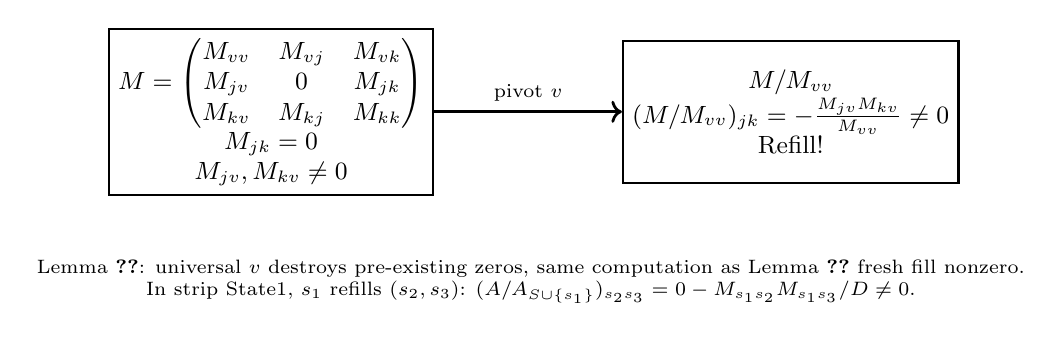
\begin{tikzpicture}[scale=1.2,
  matrix/.style={rectangle,draw,thick,minimum width=22mm,minimum height=18mm,fill=white,align=center,font=\small}
]
\node[matrix] (M) at (0,0) {$M=\begin{pmatrix}M_{vv}&M_{vj}&M_{vk}\\M_{jv}&0&M_{jk}\\M_{kv}&M_{kj}&M_{kk}\end{pmatrix}$\\$M_{jk}=0$\\$M_{jv},M_{kv}\neq0$};
\node[matrix] (M2) at (5.5,0) {$M/M_{vv}$\\$(M/M_{vv})_{jk}= -\frac{M_{jv}M_{kv}}{M_{vv}}\neq0$\\Refill!};
\draw[->,thick,line width=1pt] (M) -- (M2) node[midway,above,font=\scriptsize] {pivot $v$};
\node[font=\scriptsize,align=center] at (2.75,-1.8) {Lemma~\ref{lem:fact1}: universal $v$ destroys pre-existing zeros, same computation as Lemma~\ref{lem:fresh} fresh fill nonzero.\\In strip State1, $s_1$ refills $(s_2,s_3)$: $(A/A_{S\cup\{s_1\}})_{s_2s_3}=0-M_{s_1s_2}M_{s_1s_3}/D\neq0$.};
\end{tikzpicture}
\end{adjustbox}
\caption[The refill phenomenon]{Refill phenomenon Lemma~\ref{lem:fact1}: $(M/M_{vv})_{jk}=-M_{jv}M_{kv}/M_{vv}\neq0$ nonzero even if $M_{jk}=0$ and legs nonzero. A universal vertex destroys pre-existing zeros, just as fresh fill is nonzero at creation. This is
what clears the exceptional zero in State~1 of the strip induction via END. It does \emph{not} apply
to the separator pair of a clique sum, where the offending pivot creates the zero rather than
inheriting it (Question~\ref{q:cliquesum}).}
\label{fig:refill}
\end{figure}


\begin{lemma}[Dense Safety]\label{lem:dense}
Let $M=A/A_S$ be such that every pair of survivors $R=V\setminus S$ is nonzero in $M$, and let
$\{p,q\}$ maximize $t^{(S)}_{pq}$ over the pairs with $M_{pq}\neq0$. Then $C_p(S)$ does not cover $q$.
\end{lemma}

\begin{proof}
Write $t_{\max}=t^{(S)}_{pq}$ and suppose that $C_p(S)$ covers $q$, so that $(q,k)\in C_p(S)$ for some
survivor $k\notin\{p,q\}$. By Lemma~\ref{lem:additive},
$t^{(S)}_{qk}=t^{(S)}_{pq}+t^{(S)}_{pk}$, and $t^{(S)}_{pk}>0$ by Definition~\ref{def:t} because
$M_{pk}\neq0$. Hence $t^{(S)}_{qk}>t_{\max}$. On the other hand $M_{qk}\neq0$ by hypothesis, so
$\{q,k\}$ is one of the pairs over which the maximum was taken and $t^{(S)}_{qk}\le t_{\max}$. The two
inequalities are incompatible, so $C_p(S)$ does not cover $q$.
\end{proof}

\begin{remark}\label{rem:dense-universal}
Lemma~\ref{lem:dense} is applied below with $p$ universal in $M$, which is how it arises in the strip
and fan arguments, but universality plays no role in the proof: the density hypothesis on $R$ is
what is used.
\end{remark}

\begin{lemma}[Universal Successor]\label{lem:univsucc}
Let $M=A/A_S$ with survivors $R$, let $p$ be universal in $M$, and let $q\in R\setminus\{p\}$ be such
that $p$ is a weakest neighbour of $q$, that is
$t^{(S)}_{pq}=\max\{t^{(S)}_{qx}:M_{qx}\neq0\}$. Then $q$ is universal in $M/M_{pp}$.
\end{lemma}

\begin{proof}
Let $k\in R\setminus\{p,q\}$; we must show $(M/M_{pp})_{qk}\neq0$. If $M_{qk}=0$, then since $p$ is
universal in $M$, Lemma~\ref{lem:fact1} gives $(M/M_{pp})_{qk}=-M_{qp}M_{kp}/M_{pp}\neq0$. If instead
$M_{qk}\neq0$, then $t^{(S)}_{qk}$ is finite, and $(M/M_{pp})_{qk}=0$ would be a cancellation, so
Lemma~\ref{lem:additive} would give
$t^{(S)}_{qk}=t^{(S)}_{pq}+t^{(S)}_{pk}>t^{(S)}_{pq}$, using $t^{(S)}_{pk}>0$. That contradicts the
maximality of $t^{(S)}_{pq}$ among the $t^{(S)}_{qx}$. In both cases
$(M/M_{pp})_{qk}\neq0$, so $q$ is universal in $M/M_{pp}$.
\end{proof}

\begin{lemma}[Refill Lemma]\label{lem:refill}
Assume $\omega(G_A)\le3$. Let $\{j,k,u\}$ and $\{j,k,w\}$ be two distinct triangles of $G_A$ sharing
the edge $\{j,k\}$, so that $A_{jw}\neq0$ and $A_{kw}\neq0$, and suppose that $u$ cancels $(j,k)$.
Then $A_{uw}=0$; moreover, writing $M=A/A_{\{u\}}$, we have $M_{jw}=A_{jw}\neq0$ and
$M_{kw}=A_{kw}\neq0$, and
\[(M/M_{ww})_{jk}=-\frac{A_{jw}A_{kw}}{M_{ww}}\neq0.\]
That is, pivoting at $w$ restores the entry that $u$ destroyed.
\end{lemma}

\begin{proof}
Suppose $A_{uw}\neq0$. The six pairs among $u,j,k,w$ would then all be nonzero: $\{j,k\}$, $\{u,j\}$
and $\{u,k\}$ because $\{j,k,u\}$ is a triangle, $\{j,w\}$ and $\{k,w\}$ because $\{j,k,w\}$ is a
triangle, and $\{u,w\}$ by supposition. Thus $\{u,j,k,w\}$ would be a clique of $G_A$ on four
vertices, giving $\omega(G_A)\ge4$ and contradicting the hypothesis. Hence $A_{uw}=0$.

Now pivot at $u$. By Definition~\ref{def:pivot},
$M_{jw}=A_{jw}-A_{ju}A_{wu}/A_{uu}=A_{jw}$, since $A_{wu}=A_{uw}=0$, and likewise $M_{kw}=A_{kw}$;
both are nonzero by hypothesis. Since $u$ cancels $(j,k)$ we have $M_{jk}=0$. Pivoting at $w$
therefore gives
\[
  (M/M_{ww})_{jk}=M_{jk}-\frac{M_{jw}M_{kw}}{M_{ww}}=-\frac{A_{jw}A_{kw}}{M_{ww}},
\]
which is nonzero because the two legs are nonzero and $M_{ww}>0$ by positive definiteness of $M$.
\end{proof}

\begin{lemma}[Prefix Lemma]\label{lem:prefix}
Let $S$ be a level and suppose $(A/A_S)_{jk}=0$ for a pair with $\{j,k\}\in G_S$. Then there exists
$v\in S$ with $\{j,v\},\{k,v\}\in G_{S\setminus\{v\}}$.
\end{lemma}

\begin{proof}
We argue by induction on $|S|$.

If $S=\emptyset$ the hypothesis is vacuous: $\{j,k\}\in G_\emptyset=G_A$ means $A_{jk}\neq0$, whereas
$(A/A_\emptyset)_{jk}=A_{jk}=0$, so there is nothing to prove.

Let $|S|\ge1$, write $S=S'\cup\{v\}$ where $v$ is the vertex of $S$ eliminated last, and recall from
Lemma~\ref{lem:quotient} that this decomposition may be made for any choice of last vertex. There are
two cases.

If $\{j,v\}\in G_{S'}$ and $\{k,v\}\in G_{S'}$, then $v$ is the required witness, because
$S\setminus\{v\}=S'$.

Otherwise one of the two pairs is absent from $G_{S'}$; by the symmetry of $j$ and $k$ we may assume
$\{j,v\}\notin G_{S'}$. Since the numeric pattern is contained in the symbolic one
(Definition~\ref{def:numeric}), this forces $(A/A_{S'})_{jv}=0$, so Lemma~\ref{lem:zeroleg} gives
$(A/A_S)_{jk}=(A/A_{S'})_{jk}$, and the zero was therefore already present at level $S'$. We claim
moreover that $\{j,k\}\in G_{S'}$. Indeed, if $\{j,k\}\notin G_{S'}$ then $\{j,k\}$ is a fill edge
created by $v$, which by the definition of the elimination game requires both $\{j,v\}$ and $\{k,v\}$
to lie in $G_{S'}$, contrary to the case assumption. The inductive hypothesis applied at level $S'$
now yields a vertex $v'\in S'$ with $\{j,v'\},\{k,v'\}\in G_{S'\setminus\{v'\}}$, and $v'\in S$, which
completes the induction.
\end{proof}

\begin{corollary}\label{cor:tri-nec}
If $(A/A_S)_{jk}=0$ with $\{j,k\}\in G_S$, then $\{j,k\}$ lies in a triangle of the fill graph. In
particular, only an edge that lies in a triangle of the fill graph can ever cancel.
\end{corollary}

\begin{proof}
Let $v\in S$ be the vertex supplied by Lemma~\ref{lem:prefix}, so that $\{j,v\}$ and $\{k,v\}$ are
edges of $G_{S\setminus\{v\}}$ while $\{j,k\}$ is an edge of $G_S$. Fix an ordering $\sigma$ that
enumerates $S\setminus\{v\}$ first, then $v$, then the survivors in any order. Every edge of
$G_{S\setminus\{v\}}$ and of $G_S$ is an edge of $G^+_\sigma$, because the fill graph accumulates the
edges of $G_A$ together with all fill created along the game and never deletes one
(Definition~\ref{def:fillgraph}). Hence $\{j,k\}$, $\{j,v\}$ and $\{k,v\}$ are all edges of
$G^+_\sigma$, so $\{j,k,v\}$ is a triangle of $G^+_\sigma$ containing $\{j,k\}$.
\end{proof}

\begin{lemma}[Fresh fill is nonzero when created]\label{lem:fresh}
Let $S$ be a level, let $v\in V\setminus S$, and let $j,k\in V\setminus(S\cup\{v\})$ be distinct with
$\{j,v\},\{k,v\}\in G_S$ but $\{j,k\}\notin G_S$, so that $\{j,k\}$ is a fill edge created by $v$.
Then $(A/A_S)_{jk}=0$, and
\[
  (A/A_{S\cup\{v\}})_{jk}=-\frac{(A/A_S)_{jv}(A/A_S)_{kv}}{(A/A_S)_{vv}} .
\]
If in addition both legs are nonzero, that is $(A/A_S)_{jv}\neq0$ and $(A/A_S)_{kv}\neq0$, then this
entry is nonzero: fresh fill is nonzero at the moment of its creation. It may of course cancel at a
later level.
\end{lemma}

\begin{proof}
Since the numeric pattern is contained in the symbolic one (Definition~\ref{def:numeric}), the
hypothesis $\{j,k\}\notin G_S$ gives $(A/A_S)_{jk}=0$. Pivoting at $v$ and using
Definition~\ref{def:pivot},
\[
  (A/A_{S\cup\{v\}})_{jk}=(A/A_S)_{jk}-\frac{(A/A_S)_{jv}(A/A_S)_{kv}}{(A/A_S)_{vv}}
  =-\frac{(A/A_S)_{jv}(A/A_S)_{kv}}{(A/A_S)_{vv}},
\]
which is the displayed formula. If both legs are nonzero then the numerator is nonzero, and
$(A/A_S)_{vv}>0$ because $A/A_S$ is positive definite, so the quotient is nonzero.
\end{proof}

\begin{corollary}[Closure form of fresh fill]\label{cor:fresh-closure}
With $S,v,j,k$ as in Lemma~\ref{lem:fresh}, if the slot $(S\cup\{v\},j,k)$ is active then at least one
of the slots $(S,j,v)$ and $(S,k,v)$ is active.
\end{corollary}

\begin{proof}
By the displayed formula of Lemma~\ref{lem:fresh}, the entry $(A/A_{S\cup\{v\}})_{jk}$ vanishes only
if the product $(A/A_S)_{jv}(A/A_S)_{kv}$ vanishes, and hence only if one of its factors does.
\end{proof}

\begin{lemma}[Nesting Lemma]\label{lem:nesting}
Let $S$ be a level and let $i,j,k\in V\setminus S$ be distinct. If the slots $(S,j,k)$ and
$(S\cup\{i\},j,k)$ are both active, then at least one of the slots $(S,j,i)$ and $(S,k,i)$ is active.
\end{lemma}

\begin{proof}
By Definition~\ref{def:pivot},
\[
  (A/A_{S\cup\{i\}})_{jk}=(A/A_S)_{jk}-\frac{(A/A_S)_{ji}(A/A_S)_{ki}}{(A/A_S)_{ii}} .
\]
The left-hand side is zero because $(S\cup\{i\},j,k)$ is active, and the first term on the right is
zero because $(S,j,k)$ is active. Hence
$(A/A_S)_{ji}(A/A_S)_{ki}/(A/A_S)_{ii}=0$, and since the pivot value $(A/A_S)_{ii}$ is positive the
product $(A/A_S)_{ji}(A/A_S)_{ki}$ vanishes. A product of real numbers vanishes only if one factor
does, so $(A/A_S)_{ji}=0$ or $(A/A_S)_{ki}=0$, which says that $(S,j,i)$ or $(S,k,i)$ is active.
\end{proof}


\begin{definition}[Arc digraph of a slot family]\label{def:arcdigraph}
Let $S$ be a level, let $A\succ0$, and let $H$ be a family of slots at the levels $S\cup\{i\}$ for
$i\in V\setminus S$, whose imposed relations $t^{(S)}_{jk}=t^{(S)}_{ji}+t^{(S)}_{ki}$ are those
supplied by Lemma~\ref{lem:additive}. The \emph{arc digraph} $D(H)$ has as its vertices the pairs
$\{j,k\}$ of survivors with $(A/A_S)_{jk}\neq0$, and for each imposed relation of $H$ it has the two
arcs
\[
  \{j,k\}\to\{j,i\}\qquad\text{and}\qquad \{j,k\}\to\{k,i\},
\]
included only when the target pair is itself nonzero in $A/A_S$; if a target pair is zero then
$t^{(S)}=+\infty$ there and no arc is added. Note that $D(H)$ depends on $A$ as well as on $H$, since
which pairs are nonzero in $A/A_S$ is a numeric matter and not determined by the pattern alone.
\end{definition}


\begin{lemma}[General Cycle Lemma]\label{lem:cycle}
Fix a level $S$ and let $H$ be a family of slots at levels $S\cup\{i\}$, $i\in V\setminus S$, whose
imposed relations are $t^{(S)}_{jk}=t^{(S)}_{ji}+t^{(S)}_{ki}$ in the sense of
Lemma~\ref{lem:additive}. If the associated arc digraph $D(H)$ of Definition~\ref{def:arcdigraph}
contains a directed cycle, then $H$ is infeasible: no positive solution $t^{(S)}>0$ exists.
\end{lemma}


\begin{proof}
Each imposed relation $t^{(S)}_{jk}=t^{(S)}_{ji}+t^{(S)}_{ki}$ has both summands strictly positive
(Definition~\ref{def:t}), so $t^{(S)}_{jk}>t^{(S)}_{ji}$ and $t^{(S)}_{jk}>t^{(S)}_{ki}$: every arc of
$D(H)$ strictly decreases the value of $t^{(S)}$. A directed cycle would therefore give
$t^{(S)}_x>\cdots>t^{(S)}_x$, which is impossible. Hence no positive solution exists.
\end{proof}

The following is the
four-vertex instance of Lemma~\ref{lem:cycle}, and it is the step invoked in the proof of the Pairing
Lemma~\ref{lem:pairing}.

\begin{lemma}[4-cycle Lemma]\label{lem:4cycle}
Let $a,b,c,d$ be four distinct survivors at a level $S$. Then the four relations
\[
t^{(S)}_{ab}=t^{(S)}_{ac}+t^{(S)}_{bc},\quad
t^{(S)}_{bc}=t^{(S)}_{bd}+t^{(S)}_{cd},\quad
t^{(S)}_{cd}=t^{(S)}_{ca}+t^{(S)}_{da},\quad
t^{(S)}_{da}=t^{(S)}_{db}+t^{(S)}_{ab}
\]
cannot hold simultaneously; that is, the corresponding family of four slots is infeasible.
\end{lemma}
\begin{proof}
The four relations contribute the arcs $\{a,b\}\to\{b,c\}\to\{c,d\}\to\{d,a\}\to\{a,b\}$ of
Definition~\ref{def:arcdigraph}, a directed cycle, so Lemma~\ref{lem:cycle} applies. Concretely,
$t^{(S)}_{ab}>t^{(S)}_{bc}>t^{(S)}_{cd}>t^{(S)}_{da}>t^{(S)}_{ab}$, a contradiction.
\end{proof}

\begin{lemma}[Monotone Lemma]\label{lem:monotone}
Fix a pattern $G$. If $H$ is unrealizable for $G$, then every superset $H'\supseteq H$ is unrealizable
for $G$. Equivalently, in contrapositive form: if $H'$ is realizable for $G$ then so is $H$.
\end{lemma}
\begin{proof}
We prove the contrapositive. Suppose $H'$ is realizable for $G$, and let $A\succ0$ with $G_A=G$ be a
matrix witnessing this, so that every slot of $H'$ is active for $A$. Since $H\subseteq H'$, every slot
of $H$ is in particular a slot of $H'$ and is therefore active for $A$ as well. The same matrix $A$
thus witnesses that $H$ is realizable for $G$, the pattern being the same on both sides. Hence $H'$
realizable for $G$ implies $H$ realizable for $G$, which is what was required.
\end{proof}
\end{aiblock}

\section{Positive results}\label{sec:positive}

\begin{aiblock}
\begin{theorem}[Forests, strong form]\label{thm:forest}
If $G_A$ is a forest, then every ordering of $V$ is clean for $A$.
\end{theorem}
\begin{proof}
For $j,k\notin S$, the Schur complement has the standard almost-principal-minor form
\[
(A/A_S)_{jk}= \frac{\det A_{S\cup\{j\},\,S\cup\{k\}}}{\det A_{S,S}},
\]
where $A_{I,J}$ denotes the submatrix with rows $I$ and columns $J$; $A_{S,S}$ is principal. In particular the expression is manifestly independent of the elimination order on $S$.

Assume $G_A$ is a forest, and fix $j,k\notin S$ with $\{j,k\}\in G_S$ (symbolic). Any two vertices
of $G_A$ are joined by \emph{at most} one simple path: none if they lie in different components, and
exactly one otherwise. By Proposition~\ref{prop:fillpath} the hypothesis $\{j,k\}\in G_S$ supplies
such a path, so the $j$--$k$ path exists and is unique; we write $\mathrm{path}(j,k)$ for its edge set
and $I$ for its interior, and $I\subseteq S$. A term of
$\det A_{S\cup\{j\},S\cup\{k\}}$ is $\pm\prod_{u}A_{u,\pi(u)}$ for a bijection
$\pi:S\cup\{j\}\to S\cup\{k\}$, and it is nonzero only if $\{u,\pi(u)\}\in E(G_A)$ or $u=\pi(u)$ for
every $u$. Regard $\pi$ as a partial permutation of $V$: it is defined on $S\cup\{j\}$ and takes values
in $S\cup\{k\}$, so the two indices that fail to match are $j$ (a source, not in the codomain) and $k$
(a sink, not in the domain). Decomposing $\pi$ accordingly, it consists of one directed path from $j$
to $k$ through vertices of $S$, together with fixed points and cycles on the remaining indices of $S$.
The path contributes $\prod_{e}A_e$ over the edges of a $j$--$k$ walk in $G_A$ with interior in $S$;
in a forest the only such walk without repeated vertices is $\mathrm{path}(j,k)$. The fixed points and
cycles involve only indices of $S\setminus I$ and are matched among themselves, and their total
contribution is precisely $\det A_{S\setminus I,S\setminus I}$. Note that this includes $2$-cycles
$A_{uv}A_{vu}=A_{uv}^2$ along genuine forest edges: such terms are legitimate and are exactly what the
determinant $\det A_{S\setminus I,S\setminus I}$ collects, which is why no claim is made that off-path
indices cannot be moved. Hence
\[
\det A_{S\cup\{j\},S\cup\{k\}} = \pm\Bigl(\prod_{e\in\mathrm{path}(j,k)} A_e\Bigr)\,\det A_{S\setminus I,S\setminus I},
\]
and therefore
\[
(A/A_S)_{jk}= \pm\frac{\bigl(\prod_{e\in\mathrm{path}(j,k)} A_e\bigr)\,\det A_{S\setminus I}}{\det A_{S}}.
\]
This is the Jones--West path formula \cite{Jones}, see Lemma~1 there for the precise expansion; both $\det A_{S\setminus I}$ and $\det A_{S}$ are principal minors of the SPD matrix $A$, hence $>0$, and every $A_e\neq0$ by the forest pattern. Thus $(A/A_S)_{jk}\neq0$. Vertices of $S$ off the path are accounted for automatically via $\det A_{S\setminus I}$, which collects all their internal matchings, and they only affect pivots, never the numerator product $\prod_{e\in\mathrm{path}(j,k)} A_e$, which is manifestly order-independent; Figure~\ref{fig:forest-path} illustrates the expansion on a
small forest. No accidental zero ever occurs, irrespective of ordering \cite{Malouche,Jones}.
\end{proof}

\begin{figure}[H]
\centering
\begin{adjustbox}{max width=\textwidth}
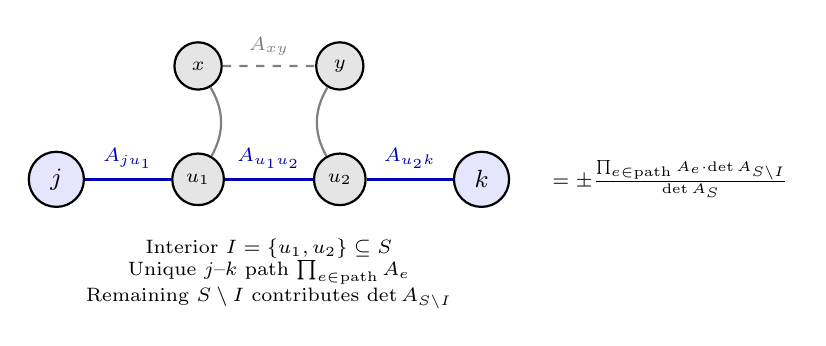
\begin{tikzpicture}[scale=1.2,
  vertex/.style={circle,draw,thick,minimum size=7mm,fill=white,font=\small},
  pathvertex/.style={circle,draw,thick,minimum size=7mm,fill=blue!10,font=\small},
  svertex/.style={circle,draw,thick,minimum size=6mm,fill=gray!20,font=\scriptsize}
]
\node[pathvertex] (j) at (0,0) {$j$};
\node[svertex] (a) at (1.5,0) {$u_1$};
\node[svertex] (b) at (3.0,0) {$u_2$};
\node[pathvertex] (k) at (4.5,0) {$k$};
\draw[thick,blue!70!black,line width=1pt] (j) -- (a) node[midway,above,font=\scriptsize] {$A_{ju_1}$};
\draw[thick,blue!70!black,line width=1pt] (a) -- (b) node[midway,above,font=\scriptsize] {$A_{u_1u_2}$};
\draw[thick,blue!70!black,line width=1pt] (b) -- (k) node[midway,above,font=\scriptsize] {$A_{u_2k}$};
% off-path matchings
\node[svertex] (x) at (1.5,1.2) {$x$};
\node[svertex] (y) at (3.0,1.2) {$y$};
\draw[thick,gray,dashed] (x) -- (y) node[midway,above,font=\scriptsize] {$A_{xy}$};
\draw[thick,gray] (x) to[bend left] (a);
\draw[thick,gray] (y) to[bend right] (b);
\node[font=\scriptsize,align=center] at (2.25,-1.0) {Interior $I=\{u_1,u_2\}\subseteq S$\\Unique $j$--$k$ path $\prod_{e\in\text{path}} A_e$\\Remaining $S\setminus I$ contributes $\det A_{S\setminus I}$};
\node[font=\scriptsize] at (6.5,0) {$=\pm\frac{\prod_{e\in\text{path}}A_e\cdot\det A_{S\setminus I}}{\det A_S}$};
\end{tikzpicture}
\end{adjustbox}
\caption[Forest path formula]{Forest path formula: $j$--$k$ with interior $S$, $I\subseteq S$. Unique path in forest gives product $\prod A_e$. Every nonzero term routes $j$ to $k$ along that path, remaining indices permute among $S\setminus I$, contributing $\det A_{S\setminus I}$ collecting off-path matchings $A_{xy}^2$. Vertices of $S$ off path accounted via that determinant, only pivots affected.}
\label{fig:forest-path}
\end{figure}

\begin{remark}
    In the statement of the theorem, $A$ is not assumed to be irreducible. If $A$ is irreducible, $G_A$ is a forest if and only if $G_A$ is a tree. Malouche and Rajaratnam's covariance-faithfulness theorem is the tree case; the forest statement follows block-wise. The corresponding statement for concentration graphs, rather than covariance graphs, is due to Becker, Geiger and Meek~\cite{Becker}.
\end{remark}

\begin{definition}[2-path strip]\label{def:strip}
For $k\ge3$, the $2$-path strip on vertices $v_1,\dots,v_k$ is the graph $P$ whose edge set is exactly
\[
E(P)=\bigl\{\{v_i,v_{i+1}\}:1\le i\le k-1\bigr\}\cup\bigl\{\{v_i,v_{i+2}\}:1\le i\le k-2\bigr\},
\]
the first family called \emph{boundary edges} and the second \emph{diagonal edges}; its triangles are $T_i=\{v_i,v_{i+1},v_{i+2}\}$ for $1\le i\le k-2$. We say $G_A$ is a $2$-path strip if $G_A=P$ for some such labelling; in particular all listed edges are original pattern edges, not fill.
\end{definition}

\begin{definition}[Strip state]\label{def:strip-state}
A \emph{strip state} is a pair $(S,P)$ where $S\subseteq V$ is a level
(Remark~\ref{rem:level-stage}) and $P$ is the graph that $G_S$ induces on the survivors
$V\setminus S$, assumed to be a $2$-path strip on $k=|V\setminus S|$ vertices. Note that $P$ is taken
in the symbolic graph $G_S$, not in $G_A$: after a SECOND move the strip uses a fill edge. We write
its left end as $s_1=v_1,s_2=v_2,s_3=v_3,s_4=v_4$; this names four particular survivors and carries no
assumption that $k=4$ (the right end is symmetric, and we treat only the left). For a $2$-path strip this $P$ is itself a $2$-path strip, except after a SECOND move it uses the fill edge $(s_1,s_4)$, which is not an edge of $G_A$ but is an edge of $G_S$ by Lemma~\ref{lem:fresh}. The state is
\begin{itemize}
\item \emph{State~0} if every boundary and diagonal edge of $P$ (including the fill edge $(s_1,s_4)$ when present) is nonzero in $A/A_S$;
\item \emph{State~1} if exactly one pair is zero in $A/A_S$, namely $(s_2,s_3)$, and every other boundary and diagonal edge of $P$ is nonzero in $A/A_S$.
\end{itemize}
\end{definition}

\begin{definition}[Moves on a strip state]\label{def:strip-moves}
Let $(S,P)$ be a strip state with $k\ge4$ survivors. Both moves below are pivots in the sense of
Definition~\ref{def:pivot}, and both are the named moves forward-declared in
Definition~\ref{def:strategy}:
\begin{itemize}
\item \emph{END} pivots $s_1$. Since $N(s_1)=\{s_2,s_3\}$ is an edge of $P$, \emph{no fill is created}, and \emph{the only pair updated is $(s_2,s_3)$}.
\item \emph{SECOND} pivots $s_2$. Since $N(s_2)=\{s_1,s_3,s_4\}$, \emph{exactly one fill edge $(s_1,s_4)$ is created}; the pairs updated are $(s_1,s_3)$, $(s_1,s_4)$, $(s_3,s_4)$, and the survivors $V\setminus(S\cup\{s_2\})$ again carry a $2$-path strip, namely $v_1,v_3,v_4,\dots,v_k$ in that order: the old diagonal $v_1v_3$ becomes a boundary edge, the new fill edge $v_1v_4$ becomes a diagonal, and no other pair is affected. Its left end is $v_1,v_3,v_4$, together with $v_5$ when $k\ge5$; for $k=4$ the resulting strip is the triangle $\{v_1,v_3,v_4\}$, which is the base case of the induction.
\end{itemize}
\end{definition}

\begin{remark}[PEO-insufficiency witness]\label{rem:peo-fail}
There exists a $2$-path of $5$ triangles where $23$ of $400$ adversarial SPD realizations have zero clean simplicial vertices, so a pure PEO strategy that never creates fill fails. Hence the induction must sometimes use SECOND to create fill. That sampling run is not included in the ancillary material; the script \texttt{peo\_insufficiency.py} (Appendix~\ref{app:code-peo}) instead checks one such realization in exact arithmetic: neither simplicial vertex is a clean pivot, all $96$ perfect elimination orderings of the pattern are unclean, and $3228$ of the $5040$ orderings, each creating fill, are clean, as Theorem~\ref{thm:positives}(i) guarantees for strips.
\end{remark}

\begin{definition}\label{def:clean_continuation}
    Let $(S, P)$ be a strip state. A continuation of $(S, P)$ is an ordering $\tau = (p_1,\dots, p_k)$ of the survivors $V\setminus S$, and we write $S_0 = S, S_i = S \cup \{p_1, \dots, p_i\}$. The continuation $\tau$ is clean if for every $i = 1, \dots, k$ and every survivor $x \in V\setminus S_i$ with $\{p_i, x\} \in G_{S_{i-1}}$, we have $(A / A_{S_{i-1}})_{p_i x} \neq 0$. We say $(S, P)$ admits a clean continuation if some continuation of it is clean.
\end{definition}

\begin{theorem}[Strips, fans, one-triangle, edge-disjoint triangles]\label{thm:positives}
Conjecture~\ref{conj:1} holds, and hence (Definition~\ref{def:strategy}) an adaptive clean ordering exists, for (i) 2-path strips and dominating-vertex fans, (ii) chordal graphs with exactly one triangle, and (iii) chordal graphs with $\omega\le3$ and pairwise edge-disjoint triangles. For none of these classes does a fixed ordering suffice (Remark~\ref{rem:no-fixed}).
\end{theorem}
\begin{proof}[Proof of (i), strips and fans]
We prove by induction on $k=|V\setminus S|$ that a strip state $(S,P)$ admits a clean continuation and that States~0 and~1 are preserved. For $k=3$ there are two cases, according to the state. In State~0 all three pairs of the triangle
$\{s_1,s_2,s_3\}$ are nonzero, so Lemma~\ref{lem:tri} applies: at most one apex route cancels, and at
least two of the three vertices zero no pair of the triangle. Pivot such a clean apex; the pivot is
clean because its two entries among the survivors are nonzero, and the surviving pair is nonzero
(otherwise it would lie in the cancellation graph of that apex), so the final $2\times2$ Schur
complement is clean. In State~1 the pair $(s_2,s_3)$ is zero while $(s_1,s_2)$ and $(s_1,s_3)$ are
nonzero, so Lemma~\ref{lem:tri} does not apply and the argument just given is unavailable. Pivot
$s_1$ instead: it is clean because both of its entries among the survivors are nonzero, and it
restores $(s_2,s_3)$ by the computation displayed in the State~1 case below, leaving a $2\times2$
Schur complement whose off-diagonal entry is nonzero. Both cases are needed, because a State~1 strip
on three vertices does arise: a SECOND move at $k=4$ can leave the exceptional zero at the new
$(s_2,s_3)$.

Inductive step: let $(S,P)$ be a strip state with left end $s_1=v_1,s_2=v_2,s_3=v_3,s_4=v_4$ (right end symmetric), $k\ge4$. Distinguish:

\begin{itemize}
\item \emph{State~0 and $(s_2,s_3)\notin C_{s_1}(S)$:} END at $s_1$. Since $N(s_1)=\{s_2,s_3\}$ is an edge, no fill is created and the only pair updated is $(s_2,s_3)$, which is nonzero by hypothesis $(s_2,s_3)\notin C_{s_1}(S)$. The pivot reads $(s_1,s_2),(s_1,s_3)$, both nonzero in State~0, hence clean. Result is State~0 on $k-1$ vertices.

\item \emph{State~0 and $(s_2,s_3)\in C_{s_1}(S)$:} SECOND at $s_2$. Note $(s_2,s_3)$ is nonzero at the time $s_2$ is pivoted, because $s_1$ has not been eliminated yet — this subtle point ensures the pivot itself is clean. The pairs updated are $(s_1,s_3)$, $(s_1,s_4)$ (fill), $(s_3,s_4)$. Lemma~\ref{lem:fresh} gives $(s_1,s_4)=-(A/A_S)_{s_2,s_1}(A/A_S)_{s_2,s_4}/(A/A_S)_{s_2s_2}\neq0$. Since $s_1$ zeroes $(s_2,s_3)$ by assumption, Lemma~\ref{lem:tri} in triangle $\{s_1,s_2,s_3\}$ implies $s_2$ cannot zero $(s_1,s_3)$; hence $(s_1,s_3)\neq0$ after $s_2$. Only $(s_3,s_4)$ may become zero, which is exactly the new $(s_2,s_3)$ in the remaining strip with vertices $s_1,s_3,s_4,s_5,\dots$. Thus we move to State~0 if $(s_3,s_4)$ stays nonzero, otherwise to State~1 with zero at new $(s_2,s_3)$. In either case the pivot $s_2$ is clean because $(s_2,s_1),(s_2,s_3),(s_2,s_4)$ are all nonzero in State~0 before $s_1$ is gone.

\item \emph{State~1:} END at $s_1$. The exceptional zero is at $(s_2,s_3)$, not at $(s_1,s_2)$. Removing $s_1$ does \emph{not} remove that pair; if we pivoted $s_2$ next we would commit a zero to $L$ and be dirty. Instead END refills it:
\[
(A/A_{S\cup\{s_1\}})_{s_2s_3}=0-\frac{(A/A_S)_{s_1s_2}(A/A_S)_{s_1s_3}}{(A/A_S)_{s_1s_1}}\neq0,
\]
because both legs are nonzero in State~1 by definition and $(A/A_S)_{s_1s_1}>0$ by positive
definiteness. This is the pivot update of Definition~\ref{def:pivot} applied to a pair that is
already zero, the same computation that appears in Lemma~\ref{lem:fact1} and in
Lemma~\ref{lem:fresh}. Note that Lemma~\ref{lem:fact1} is not being invoked: $s_1$ need not be
universal in $A/A_S$, since a strip with $k\ge4$ survivors has survivors not adjacent to $s_1$. What
makes the two legs nonzero here is the strip state, not domination of the survivors by $s_1$. It is
the refill phenomenon of Section~\ref{sec:intro-exist} doing constructive work. The pivot $s_1$ reads $(s_1,s_2),(s_1,s_3)$, both nonzero, hence clean. After END the state is State~0 on $k-1$ vertices.
\end{itemize}
The table is exhaustive, State~0 and State~1 are preserved, and $k$ drops by one per move,
terminating at the $k=3$ base case. Figure~\ref{fig:fourmoves} shows the two moves on a strip of five
triangles, and Figure~\ref{fig:strip-machine} collects the three cases above as a transition diagram.

\begin{figure}[H]
\centering
\begin{adjustbox}{max width=\textwidth}
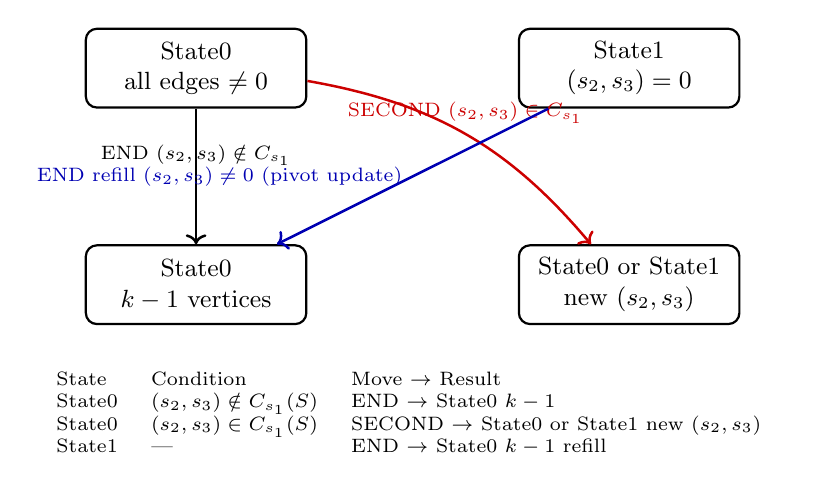
\begin{tikzpicture}[scale=1.1,
  state/.style={rectangle,draw,thick,rounded corners,minimum width=28mm,minimum height=10mm,fill=white,font=\small,align=center},
  arrow/.style={->,thick,line width=0.9pt}
]
\node[state] (s0) at (0,0) {State0\\all edges $\neq0$};
\node[state] (s1) at (5,0) {State1\\$(s_2,s_3)=0$};
\node[state] (s0b) at (0,-2.5) {State0\\$k-1$ vertices};
\node[state] (s0c) at (5,-2.5) {State0 or State1\\new $(s_2,s_3)$};

\draw[arrow] (s0) -- node[above,font=\scriptsize] {END $(s_2,s_3)\notin C_{s_1}$} (s0b);
\draw[arrow,red!80!black] (s0) to[bend left=20] node[above,font=\scriptsize] {SECOND $(s_2,s_3)\in C_{s_1}$} (s0c);
\draw[arrow,blue!70!black] (s1) -- node[left,font=\scriptsize] {END refill $(s_2,s_3)\neq0$ (pivot update)} (s0b);
\node[font=\scriptsize,align=left] at (2.5,-4) {
\begin{tabular}{lll}
State & Condition & Move $\to$ Result\\
State0 & $(s_2,s_3)\notin C_{s_1}(S)$ & END $\to$ State0 $k-1$\\
State0 & $(s_2,s_3)\in C_{s_1}(S)$ & SECOND $\to$ State0 or State1 new $(s_2,s_3)$\\
State1 & --- & END $\to$ State0 $k-1$ refill\\
\end{tabular}
};
\end{tikzpicture}
\end{adjustbox}
\caption[Strip state machine]{Strip state machine: $k\ge4$ left end $s_1,s_2,s_3,s_4$. END simplicial no fill only pair updated $(s_2,s_3)$; SECOND creates fill $(s_1,s_4)$ updates $(s_1,s_3),(s_1,s_4),(s_3,s_4)$, $V\setminus(S\cup\{s_2\})$ again strip with $s_1,s_3,s_4,s_5$ as new $s_1\ldots s_4$. Table exhaustive. Subtle point $(s_2,s_3)$ nonzero at time $s_2$ pivoted because $s_1$ not yet eliminated. The State~1 $\to$ State~0 END transition is the pivot update of Definition~\ref{def:pivot}, not an application of Lemma~\ref{lem:fact1} (Fact~1): $s_1$ need not be universal.}
\label{fig:strip-machine}
\end{figure}

\begin{figure}[H]
\centering
\begin{adjustbox}{max width=\textwidth}
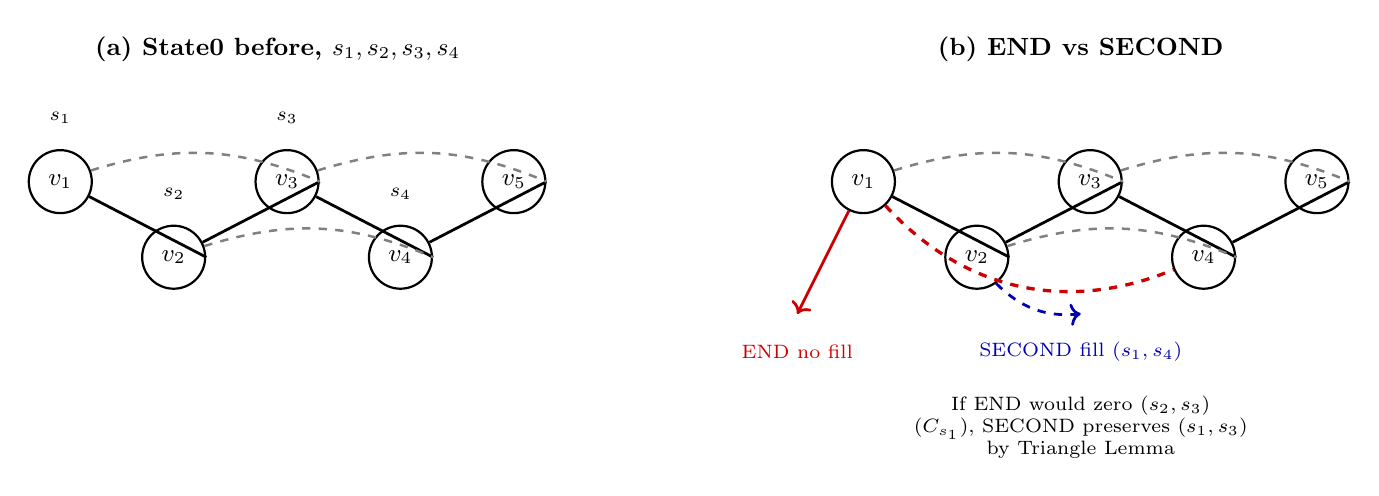
\begin{tikzpicture}[scale=1.2,
  vertex/.style={circle,draw,thick,minimum size=8mm,fill=white,font=\small},
  boundary/.style={black,thick,line width=1pt},
  diagonal/.style={black!50,thick,dashed,line width=0.9pt},
  fillstar/.style={red!80!black,ultra thick,dashed,line width=1.2pt},
  endarrow/.style={red!80!black,thick,->,line width=1pt},
  secondarrow/.style={blue!70!black,thick,dashed,->,line width=1pt}
]
% Left panel State0 before
\begin{scope}
\node at (3.5,2.2) {\small\textbf{(a) State0 before, $s_1,s_2,s_3,s_4$}};
\foreach \i in {1,...,5}{
  \pgfmathsetmacro\x{\i*1.2}
  \pgfmathsetmacro\y{mod(\i,2)*0.8}
  \node[vertex] (a\i) at (\x,\y) {$v_{\i}$};
}
\foreach \i in {1,...,4}{
  \pgfmathsetmacro\j{\i+1}
  \draw[boundary] (a\i) -- (a\j);
}
\foreach \i in {1,...,3}{
  \pgfmathsetmacro\j{\i+2}
  \draw[diagonal] (a\i) to[bend left=20] (a\j);
}
\node[above=2mm of a1, font=\scriptsize] {$s_1$};
\node[above=2mm of a2, font=\scriptsize] {$s_2$};
\node[above=2mm of a3, font=\scriptsize] {$s_3$};
\node[above=2mm of a4, font=\scriptsize] {$s_4$};
\end{scope}

% Right panels: END vs SECOND
\begin{scope}[xshift=8.5cm]
\node at (3.5,2.2) {\small\textbf{(b) END vs SECOND}};
\foreach \i in {1,...,5}{
  \pgfmathsetmacro\x{\i*1.2}
  \pgfmathsetmacro\y{mod(\i,2)*0.8}
  \node[vertex] (b\i) at (\x,\y) {$v_{\i}$};
}
\foreach \i in {1,...,4}{
  \pgfmathsetmacro\j{\i+1}
  \draw[boundary] (b\i) -- (b\j);
}
\foreach \i in {1,...,3}{
  \pgfmathsetmacro\j{\i+2}
  \draw[diagonal] (b\i) to[bend left=20] (b\j);
}
% END no fill
\node[red!80!black,font=\scriptsize] at (0.5,-1.0) {END no fill};
\draw[endarrow] (b1) -- (0.5,-0.6);
% SECOND fill (s1,s4)
\node[blue!70!black,font=\scriptsize,align=center] at (3.5,-1.0) {SECOND fill $(s_1,s_4)$};
\draw[secondarrow] (b2) to[bend right=25] (3.5,-0.6);
\draw[fillstar] (b1) to[bend right=35] (b4);
\node[font=\scriptsize,align=center] at (3.5,-1.8) {If END would zero $(s_2,s_3)$\\($C_{s_1}$), SECOND preserves $(s_1,s_3)$\\by Triangle Lemma};
\end{scope}
\end{tikzpicture}
\end{adjustbox}
\caption[2-path strip, five triangles]{2-path strip $5$ triangles $v_1\ldots v_7$, $T_i=(v_i,v_{i+1},v_{i+2})$. Boundary solid thick $1$pt, diagonal dashed $0.9$pt. (a) State0 before with $s_1,s_2,s_3,s_4$. (b) END simplicial no fill vs SECOND one fill $(s_1,s_4)$ curved thick dashed red leaves 2-path. If END would zero $(s_2,s_3)$ ($C_{s_1}$), SECOND preserves $(s_1,s_3)$ by Triangle Lemma. Larger canvas, State0/1 illustrated before/after.}
\label{fig:fourmoves}
\end{figure}


Fans (dominating-vertex fan): $G$ has a center $c$ adjacent to all vertices $v_1,\dots,v_k$ of a path, plus boundary edges $v_i v_{i+1}$ (no diagonals initially). Then $N(v_1)=\{c,v_2\}$ and $N(v_2)=\{c,v_1,v_3\}$ in $G_A$, because the strip diagonals $v_i v_{i+2}$ are not present, and $c$--$v_2$ is an edge, so $v_1$ is simplicial. In general $v_1$ is simplicial with clique $\{c,v_2\}$, so END at $v_1$ creates no fill and updates only $(c,v_2)$. Eliminating $v_1$ leaves a fan on $k-1$ path vertices. Eliminating $v_2$ next has $N(v_2)=\{c,v_1,v_3\}$ (or $\{c,v_3\}$ if $v_1$ gone) and creates exactly one fill edge $(v_1,v_3)$ when $v_1$ still present, which becomes a diagonal that will be present as fill in subsequent states. Thus diagonals do appear as fill once peeling starts, which is why the fan argument is not verbatim the strip's but is analogous.

We maintain fan states: $(S,P)$ where $P$ is $G_S$ on $V\setminus S$, which is a fan possibly with one extra diagonal $(s_1,s_3)$ from a previous SECOND. Invariant: all edges $c v_i$ and all path edges $v_i v_{i+1}$ (and any created diagonal) are nonzero, except possibly one exceptional pair. Define State~0: all $c v_i$ and $v_i v_{i+1}$ (and existing diagonal) nonzero; State~1: exactly one pair zero, namely $(c,s_2)$, others nonzero. Then:

\begin{itemize}
\item END at $s_1=v_1$: $N(s_1)=\{c,s_2\}$ is an edge, so no fill, only pair updated is $(c,s_2)$. If State~0 and $(c,s_2)\notin C_{s_1}(S)$, we stay State~0 on $k-1$ vertices; if $(c,s_2)\in C_{s_1}(S)$, we must pivot $s_2$ instead (next case). Pivot $s_1$ is clean because $(s_1,c),(s_1,s_2)$ nonzero.
\item SECOND at $s_2$: $N(s_2)=\{c,s_1,s_3\}$ (up to $s_4$ if diagonal present), creates fill $(s_1,s_3)$. Pairs updated are $(c,s_1),(c,s_3),(s_1,s_3)$. The fill edge $(s_1,s_3)$ is nonzero at the moment
of its creation by Lemma~\ref{lem:fresh}, its two legs $(s_2,s_1)$ and $(s_2,s_3)$ being nonzero. If
$s_1$ zeroed $(c,s_2)$, Lemma~\ref{lem:tri} in triangle $\{c,s_1,s_2\}$ gives $s_2$ cannot zero $(c,s_1)$, so $(c,s_1)$ stays nonzero. Only $(c,s_3)$ may become the new exceptional $(c,s_2)$ for the remaining fan. Pivot $s_2$ is clean because $(s_2,c),(s_2,s_1),(s_2,s_3)$ are nonzero at that time ($s_1$ not yet eliminated for the $(c,s_2)$ check).
\item State~1 (zero at $(c,s_2)$): END at $s_1$ refills it, since
\[
(A/A_{S\cup\{s_1\}})_{c,s_2}
 = -\frac{(A/A_S)_{s_1,c}\,(A/A_S)_{s_1,s_2}}{(A/A_S)_{s_1,s_1}}\neq0
\]
because both legs are nonzero in State~1 and $(A/A_S)_{s_1,s_1}>0$. As in the strip case this is
the pivot update of Definition~\ref{def:pivot} and not an application of Lemma~\ref{lem:fact1}: in a
fan with at least three path vertices $s_1$ is not universal. Note that $s_1$ is adjacent to both $c$
and $s_2$, which is what makes the pair $(c,s_2)$ one of the pairs this pivot updates. So State~1
$\to$ State~0 on $k-1$ vertices.
\end{itemize}
The induction terminates when a single path vertex remains. That configuration is always in
State~0: State~1 has its exceptional zero at $(c,s_2)$ and therefore needs two path vertices, so it
cannot occur with one. The unique surviving pair $(c,v)$ is then nonzero and either pivot is clean.
If $c$ is eliminated last, there is no surviving pair and no off-diagonal $L$ entry in its column, so
the step is vacuously clean (not because $C_c=\emptyset$, which would be a non-sequitur: universality says the row is nonzero, not that $c$ zeroes no pair). Induction on $k$ gives a clean ordering. Thus fans admit an adaptive clean ordering.

\end{proof}

\begin{proof}[Proof of (ii), one-triangle]
First we prove the positive claim for all chordal graphs with exactly one triangle. Let $G$ be chordal with exactly one triangle $T$. Every simplicial vertex $v\notin T$ has exactly one neighbour: if $v$ had two neighbours $x$ and
$y$, they would be adjacent to each other because $N(v)$ is a clique, so $\{v,x,y\}$ would be a
triangle, and it would be distinct from $T$ because $v\notin T$, contradicting the hypothesis that
$T$ is the only triangle. Hence eliminating $v$ creates no fill and updates no off-diagonal pair: $(A/A_S)_{jk}$ is unchanged for $j,k\neq v$, only the diagonal $(A/A_S)_{vv}$ disappears. Hence such a $v$ cannot create a zero and can be peeled cleanly irrespective of numerics. Moreover, as long as $G$ properly contains $T$ there is a simplicial vertex outside $T$ available
to peel: a chordal graph with exactly one triangle consists of $T$ with trees attached, since a cycle
other than $T$ would have a chord and so create a second triangle, and a leaf of such a tree is
simplicial and outside $T$. Peeling these vertices one at a time therefore leaves exactly $T$, a
triangle, where Lemma~\ref{lem:tri} supplies a clean apex (at most one of the three vertices is dirty, so at least two are clean). Thus an adaptive clean ordering exists for every SPD matrix with that pattern.

\end{proof}

\begin{proof}[Proof of (iii), edge-disjoint triangles]
Let $G$ be chordal with $\omega\le3$ and pairwise edge-disjoint triangles. Use the bipartite block-cut tree (blocks vs cut vertices) whose leaves are always blocks.

Consider a leaf block $B$ in this tree. If $B$ is an edge $\{c,x\}$ where $c$ is the cut vertex, then $x$ is simplicial with $N(x)=\{c\}$; eliminating $x$ creates no fill and updates no pair, so it is clean and leaves a graph in the same class.

If $B$ is a triangle $\{c,a,b\}$ where $c$ is the cut vertex (or $B$ is isolated triangle when $G$ itself is a triangle), then $a,b$ are simplicial and $N(a)=\{c,b\}$, $N(b)=\{c,a\}$ are edges. By Lemma~\ref{lem:tri} at most one of the three vertices of $B$ is dirty (zeroes a pair of $B$), so at least one of the two simplicial vertices $a,b$ is clean — pigeonhole. Choose a clean apex among $a,b$, say $a$. Then $a$ zeroes no pair of its triangle, its neighbourhood is exactly the opposite edge $\{c,b\}$ because $\omega\le3$ and edge-disjointness, so eliminating $a$ creates no fill and zeroes no pair of $B$. The remaining graph is still chordal with $\omega\le3$ and edge-disjoint triangles, with $|V|$ reduced by one (the triangle block $\{c,a,b\}$ becomes the edge block $\{c,b\}$, so the number of blocks is unchanged). Induction on $|V|$ (equivalently $|E|$) closes.
\end{proof}
\begin{remark}\label{rem:no-fixed}
    In the proof of (iii), the naive block tree that connects blocks directly fails for a star of three bridges sharing a central cut vertex: the three bridge-blocks are pairwise adjacent through the hub, so they do not form a tree; the bipartite incidence tree fixes this.

For none of the classes (i)--(iii) does a fixed ordering suffice, so the clean orderings of
Theorem~\ref{thm:positives} must depend on the matrix (Definition~\ref{def:strategy}). The simplest
witness is the triangle $K_3$, which is a $2$-path strip, a fan, a chordal graph with exactly one
triangle, and a chordal graph with $\omega\le3$ whose triangles are (trivially) edge-disjoint. For a
vertex $a$ of $K_3$ with opposite pair $\{b,c\}$, let $T^{(a)}$ have unit diagonal,
$T^{(a)}_{ab}=T^{(a)}_{ac}=1/2$ and $T^{(a)}_{bc}=1/4$. It is SPD, with leading principal minors
$1,3/4,9/16$ in the order $a,b,c$, and $(T^{(a)}/T^{(a)}_{aa})_{bc}=1/4-(1/2)(1/2)=0$. Given an ordering
$\sigma$, let $a$ be its first vertex. The pair $\{b,c\}$ is an edge, hence predicted nonzero, and it
is committed at level $\{a\}$, where it vanishes for $T^{(a)}$. So no fixed $\sigma$ is clean for all
three matrices.

The phenomenon is not special to complete patterns. Take the pattern $E=\{03,04,14,23,34\}$, vertices $0,\dots,4$, edges as listed, unique triangle $\{0,3,4\}$, vertex $1$ adjacent only to $4$, vertex $2$ adjacent only to $3$. This graph is chordal, has exactly one triangle and no dominating vertex. We exhibit explicit $5\times5$ SPD matrices with that zero pattern, chosen according to the ordering, to show no fixed ordering works.

For $u=0$ (first among $\{0,3,4\}$ is $0$, cancel $(3,4)$):
\[
A^{(0)}=\begin{pmatrix}
3&0&0&1&1\\
0&3&0&0&1\\
0&0&3&1&0\\
1&0&1&3&1/3\\
1&1&0&1/3&3
\end{pmatrix},
\]
Leading principal minors $3,9,27,63,147>0$ hence SPD, $(A^{(0)}/A^{(0)}_{00})_{34}=1/3-1\cdot1/3=0$.

For $u=3$ (cancel $(0,4)$): need $A_{33}A_{04}=A_{03}A_{34}$. Choose $A_{33}=2$, $A_{04}=0.5$, $A_{03}=1$, $A_{34}=1$ gives $2\cdot0.5=1$:
\[
A^{(3)}=\begin{pmatrix}
3&0&0&1&0.5\\
0&3&0&0&1\\
0&0&3&1&0\\
1&0&1&2&1\\
0.5&1&0&1&3
\end{pmatrix},
\]
Leading minors $3,9,27,36,297/4>0$ hence SPD (not diagonally dominant, so we quote minors), $(A^{(3)}/A^{(3)}_{33})_{04}=0.5-1\cdot1/2=0$.

For $u=4$ (cancel $(0,3)$): need $A_{44}A_{03}=A_{04}A_{34}$. Choose $A_{44}=2$, $A_{03}=0.5$, $A_{04}=1$, $A_{34}=1$ gives $2\cdot0.5=1$:
\[
A^{(4)}=\begin{pmatrix}
3&0&0&0.5&1\\
0&3&0&0&1\\
0&0&3&1&0\\
0.5&0&1&3&1\\
1&1&0&1&2
\end{pmatrix},
\]
Leading minors $3,9,27,279/4,297/4>0$ hence SPD, $(A^{(4)}/A^{(4)}_{44})_{03}=0.5-1\cdot1/2=0$.

Each matrix has exactly pattern $E$, exactly one triangle and no extra edges.

Now fix a permutation $\sigma$ and let $u$ be the first vertex of $\{0,3,4\}$ in $\sigma$. Pivoting
$u$ can zero the opposite pair of the triangle, but that pair is committed only when the earlier of
its two ends is pivoted, so the zero must be present at the level $S$ of the vertices preceding that
end. Two points need care. First, the pendant vertices $1$ and $2$ may precede $u$, and pivoting a
pendant changes the diagonal entry at its unique neighbour: eliminating $2$ replaces $A_{33}$ by
$A_{33}-A_{23}^2/A_{22}$, and eliminating $1$ replaces $A_{44}$ by $A_{44}-A_{14}^2/A_{11}$, while no
off-diagonal entry is affected, since a pendant has a single neighbour. Second, a pendant pivoted
after its neighbour $u$ is no longer pendant: eliminating $u$ joins it to both ends of the zeroed
pair, and pivoting it then updates that pair. The witness is therefore chosen by whether the pendant
at $u$ lies in $S$, as follows.

If $u=0$, take $A^{(0)}$. No pendant is adjacent to $0$, and the entries $A_{00},A_{03},A_{04},A_{34}$
that enter the condition $A_{00}A_{34}=A_{03}A_{04}$ are untouched by pivoting $1$ or $2$; hence the
zero at $(3,4)$ appears when $0$ is pivoted, whichever pendants precede it. It persists until the
pair is committed, since $1$ and $2$ remain pendant after $0$ is eliminated and pivoting them changes
only the diagonal entries at $4$ and $3$.

If $u=3$, the zeroed pair is $\{0,4\}$, and $S$ consists of $3$, possibly $1$ and possibly $2$.
Whether $1\in S$ does not matter: while $4$ survives, $1$ is adjacent only to $4$, so pivoting it
changes only the diagonal entry at $4$. Take $A^{(3)}$ as displayed when $2\notin S$, that is, when
$2$ does not precede both $0$ and $4$; then $(A/A_S)_{04}=(A/A_{\{3\}})_{04}=0$. Take $A^{(3)}$ with
$A_{33}=7/3$ in place of $2$ when $2\in S$. The modified matrix is SPD, with leading principal minors
$3,9,27,45,195/2$, and the compensation is exact: $7/3-A_{23}^2/A_{22}=7/3-1/3=2$, so
$(A/A_S)_{04}=(A/A_{\{2,3\}})_{04}=0$. Symmetrically, if $u=4$ the zeroed pair is $\{0,3\}$: take
$A^{(4)}$ as displayed when $1$ does not precede both $0$ and $3$, and with $A_{44}=7/3$ in place of
$2$ when it does; the minors are then $3,9,27,279/4,195/2$ and $(A/A_{\{1,4\}})_{03}=0$.

In every case the pair zeroed by $u$, an edge of $E$ and hence predicted nonzero, is zero at the
level where it is committed, so $\sigma$ is not clean for that matrix. Hence no fixed $\sigma$ is
clean for every SPD matrix with pattern $E$, whereas the peeling argument above supplies an adaptive
clean ordering for each individual matrix. Both adjustments are needed. For the displayed $A^{(3)}$
one computes $(A/A_{\{2,3\}})_{04}=-1/10\neq0$. So $\sigma=(2,3,0,1,4)$ escapes $A^{(3)}$ because
pivoting $2$ first lowers the diagonal at $3$; and $\sigma=(3,2,0,1,4)$ escapes it although pivoting
$3$ first does create the zero at $(0,4)$, because pivoting $2$ refills it before $0$ commits the pair.
In fact $\sigma$ is clean for $A^{(3)}$. This is the refill phenomenon of
Section~\ref{sec:intro-exist}, and it is why the witness is chosen by when the zeroed pair is
committed rather than by the position of $u$. The script \texttt{fixed\_ordering\_witnesses.py}
(Appendix~\ref{app:code-fixed}) checks the three matrices for $K_3$ against all $6$ orderings and
this choice of witness for $E$ against all $120$.
\end{remark}
\end{aiblock}

\section{Even counterexamples and order four}\label{sec:even}
\begin{aiblock}
\begin{theorem}[Conjecture~2 fails at order~4, $A^*$]\label{thm:Astar}
Let
\[
A^*=\begin{pmatrix}4&-2&-2&-1\\-2&4&1&2\\-2&1&4&2\\-1&2&2&4\end{pmatrix},
\]
$\operatorname{spec}(A^*)=\{9,3,3,1\}$, SPD. Then $0$ of $24$ permutations have clean first Schur complement, while $8$ of $24$ have clean full Cholesky factor. Hence Conjecture~\ref{conj:2} is false. However, $A^*$ is not a counterexample to
Conjecture~\ref{conj:1}: the refill phenomenon rescues eight of its orderings.
\end{theorem}
\begin{proof}
\emph{Positive definiteness and the spectrum.} The leading principal minors of $A^*$ are $4$, $12$,
$36$ and $81$, all positive, so $A^*\succ0$. Its characteristic polynomial factors as
\[
  \det(xI-A^*)=x^4-16x^3+78x^2-144x+81=(x-9)(x-3)^2(x-1),
\]
so $\operatorname{spec}(A^*)=\{9,3,3,1\}$.

Every off-diagonal entry of $A^*$ is nonzero, so $G_{A^*}=K_4$, and by
Proposition~\ref{prop:fillpath} every pair of distinct vertices is a predicted-nonzero position at
every level. Cleanliness therefore amounts to the statement that no committed entry vanishes, and no
fill-path bookkeeping is required.

\emph{Stage one: every ordering fails.} The first Schur complement depends only on the first pivot, so
there are four matrices to inspect rather than $24$. Pair the vertices as $\{0,3\}$ and $\{1,2\}$,
write $q$ for the partner of the first pivot $p$, and let $\{j,k\}$ be the remaining pair. In each of
the four cases the first Schur complement has a single zero, located at $(j,k)$. For $p=0$, for
instance,
\[
  A^*/A^*_{\{0\}}=\begin{pmatrix}3&0&3/2\\0&3&3/2\\3/2&3/2&15/4\end{pmatrix}
\]
on the survivors $1,2,3$, whose $(1,2)$ entry is $1-(-2)(-2)/4=0$; the three remaining cases are the
same computation after relabelling, with the zero at $(1,2)$ for $p=3$ and at $(0,3)$ for $p=1$ and
$p=2$. Since $(j,k)$ is a predicted-nonzero position, each of the $24$ orderings meets a cancellation
in its first Schur complement, and Conjecture~\ref{conj:2} fails for $A^*$.

\emph{Stage two: exactly eight orderings are clean.} Fix the first pivot $p$ and let $q$, $j$, $k$ be
as above. The only vanishing pair of $M=A^*/A^*_{\{p\}}$ is $(j,k)$, so $M_{qj}\neq0\neq M_{qk}$ and
$q$ is universal in $M$ in the sense of Definition~\ref{def:universal}. Lemma~\ref{lem:fact1} applies
to $q$ and shows that pivoting it destroys the zero; for $p=0$ and $q=3$,
\[
  (M/M_{33})_{12}=0-\frac{(3/2)(3/2)}{15/4}=-\frac35\neq0 .
\]
The pivot at $q$ is itself clean, because its committed entries $M_{qj}$ and $M_{qk}$ are nonzero, and
after it the two remaining survivors are joined by a nonzero entry, so the whole factor is clean.
Conversely, if the second pivot is $j$ or $k$ instead of $q$, then its committed column contains the
entry $(j,k)$, which is zero, and the ordering is dirty. An ordering is therefore clean precisely when
its second pivot is the partner of its first, which leaves $4\cdot1\cdot2=8$ clean orderings, namely
\[
  (0,3,1,2),\ (0,3,2,1),\ (1,2,0,3),\ (1,2,3,0),\ (2,1,0,3),\ (2,1,3,0),\ (3,0,1,2),\ (3,0,2,1).
\]
Every computation above is exact rational arithmetic. Hence $A^*$ refutes
Conjecture~\ref{conj:2} while satisfying Conjecture~\ref{conj:1}, and the mechanism separating the two
is refill.
\end{proof}
\end{aiblock}
\begin{humanblock}
\begin{theorem}[Conjecture~1 holds for $n\le4$]\label{thm:leq4}
Conjecture~\ref{conj:1} holds for $n\le4$.
\end{theorem}
\begin{proof}
The argument is elementary and uses no computation: only the pivot update of
Definition~\ref{def:pivot}, the cancellation graph of Definition~\ref{def:cancel}, and
Lemmas~\ref{lem:tri}, \ref{lem:maxedge}, \ref{lem:refill} and~\ref{lem:fresh}. Since $A$ is
irreducible, $G_A$ is connected, so it suffices to treat the connected patterns on at most four
vertices. We use two observations repeatedly.

\emph{(O1) Pivoting a vertex of surviving degree one is clean and creates no fill.} Let $p$ be a
survivor at level $S$ whose only neighbor in $G_S$ is $w$. The pairs updated by the pivot at $p$ are
those $\{j,k\}$ with $(A/A_S)_{jp}\neq0\neq(A/A_S)_{kp}$, which forces $j=k=w$; there are none. So no
entry among the survivors changes, no fill is created, and the column committed to $L$ consists of the
single entry $(A/A_S)_{pw}\neq0$.

\emph{(O2) Three survivors forming a triangle admit a clean pivot.} Let the survivors be $\{j,k,u\}$
with all three pairs nonzero. By Lemma~\ref{lem:tri} at most one of the three apex routes cancels, so
some vertex, say $u$, zeroes no pair of the triangle. Pivoting $u$ commits $(u,j)$ and $(u,k)$, both
nonzero, and leaves $(j,k)\neq0$ because $(j,k)\notin C_u(S)$; the final $2\times2$ Schur complement
is therefore clean as well.

For $n=1$ there is nothing to prove, and for $n=2$ connectedness gives $A_{01}\neq0$, so the unique
off-diagonal entry of $L$ is nonzero. The connected patterns on three vertices are the path and the
triangle: the path is handled by peeling a leaf with (O1) and then applying the case $n=2$, and the
triangle is (O2). Up to isomorphism there are six connected patterns on four vertices, which we treat
in turn.

\emph{(a) The path $P_4$ and the star $K_{1,3}$.} Both are trees, so each has a leaf; peel it by (O1)
and induct, the remaining graph being a tree on three vertices.

\emph{(b) The paw}, a triangle $\{0,1,2\}$ with a pendant $3$ attached to $0$. Pivot the pendant $3$
first. By (O1) the step is clean and alters no entry among $\{0,1,2\}$, so the survivors still form a
triangle with all three pairs nonzero, and (O2) finishes.

\emph{(c) $K_4-e$}, with vertices $\{1,2,3,4\}$ and non-edge $\{1,4\}$, so that the triangles
$\{1,2,3\}$ and $\{2,3,4\}$ share the edge $\{2,3\}$. The vertex $1$ is simplicial, since
$N(1)=\{2,3\}$ is an edge; pivoting it creates no fill and commits the nonzero entries $(1,2)$ and
$(1,3)$, so the step is clean whatever the numerics. If $(2,3)\notin C_1$, the survivors $\{2,3,4\}$
form a triangle with all pairs nonzero and (O2) finishes. If instead $(2,3)\in C_1$, then
Lemma~\ref{lem:refill} applies to the two triangles sharing $\{2,3\}$: as $\omega(G_A)=3$ we have
$A_{14}=0$, so pivoting $1$ leaves $(2,4)$ and $(3,4)$ at their original nonzero values while $(2,3)$
becomes zero. Pivot $4$ next. Its committed entries $(4,2)$ and $(4,3)$ are nonzero, so the step is
clean, and the update restores
\[
  (A/A_{\{1,4\}})_{23}=-\frac{(A/A_{\{1\}})_{24}(A/A_{\{1\}})_{34}}{(A/A_{\{1\}})_{44}}\neq0,
\]
so the final $2\times2$ Schur complement is clean.

\emph{(d) The cycle $C_4$}, say $0-1-2-3-0$. Pivot $0$. Its neighbourhood $\{1,3\}$ is not an edge, so
the pivot creates the fill pair $(1,3)$, which is nonzero by Lemma~\ref{lem:fresh} because both legs
$(0,1)$ and $(0,3)$ are original nonzero entries; those two legs are also exactly the committed
column, so the step is clean. The survivors $\{1,2,3\}$ now form a triangle with all three pairs
nonzero, and (O2) finishes.

\emph{(e) The complete graph $K_4$.} Let $(p,q)$ maximise $t^{(\emptyset)}_{pq}$ over all pairs, and
let $\{k,l\}$ be the two remaining vertices. By Lemma~\ref{lem:maxedge} no pair of $C_p$ contains
$q$, so neither $(q,k)$ nor $(q,l)$ is cancelled by $p$; and since $A$ has no zero off-diagonal
entry, the zeros present after pivoting $p$ are by Definition~\ref{def:cancel} exactly the pairs of
$C_p$. Hence at most one pair among the survivors is zero, namely possibly $(k,l)$. Pivoting $p$ is
clean, because its committed column $(p,q),(p,k),(p,l)$ consists of original nonzero entries. If
$(k,l)\notin C_p$, the survivors form a triangle with all pairs nonzero and (O2) finishes. If
$(k,l)\in C_p$, pivot $q$ next: its committed entries $(q,k)$ and $(q,l)$ are nonzero by the
preceding sentence, so the step is clean, and the update restores
\[
  (A/A_{\{p,q\}})_{kl}=0-\frac{(A/A_{\{p\}})_{qk}(A/A_{\{p\}})_{ql}}{(A/A_{\{p\}})_{qq}}\neq0,
\]
leaving a clean final $2\times2$ Schur complement.

In every case we have produced an ordering all of whose committed entries are nonzero, which is
cleanliness in the sense of Definition~\ref{def:clean}.
\end{proof}

\begin{remark}[The argument is special to order four]\label{rem:leq4-sharp}
Case~(e) is genuinely an order-four argument. With three survivors the only pair avoiding $q$ is
$\{k,l\}$, so $C_p$ can leave at most one zero behind. From five vertices onwards $C_p$ may leave
several, the case analysis branches, and an exhaustive search over blocking families would be needed
in its place; we do not carry one out here.
\end{remark}
\end{humanblock}
\begin{aiblock}
\subsection{Pairing Lemma and forced magnitudes}

\begin{definition}\label{def:involution}
    A \emph{permutation} $\pi$ of a finite set $W$ is an \emph{involution} if $\pi^2=\mathrm{id}$, and it is \emph{fixed-point-free} if $\pi(x)\neq x$ for every $x\in W$. Fixed-point-free involutions of $W$ correspond bijectively to perfect matchings of $W$, the matching pairing each $x$ with $\pi(x)$; in particular such an involution exists if and only if $|W|$ is even.

\end{definition}

\begin{lemma}[Pairing Lemma]\label{lem:pairing}
Fix a level $S$ and a set $W$ of four surviving vertices. There are $4\binom{3}{2}=12$ candidate slots
$(u,\{j,k\})$ with $u\in W$ and $\{j,k\}\subseteq W\setminus\{u\}$, one for each choice of apex together
with the pair it cancels, and $\binom{4}{2}=6$ variables $t^{(S)}_{jk}$, one for each pair inside $W$.
Then:
\begin{enumerate}
\item every feasible set of these slots has at most four elements;
\item a feasible set of four slots that uses all four vertices of $W$ as apexes is a fixed-point-free
      involution of $W$: the four vertices split into two pairs, and each vertex cancels the pair
      opposite its own;
\item all three such configurations, one for each of the three partitions of $W$ into two pairs, are
      feasible.
\end{enumerate}
\end{lemma}
\begin{proof}
Throughout, a slot $(u,p)$ with $p=\{j,k\}$ imposes the relation
$t^{(S)}_{jk}=t^{(S)}_{uj}+t^{(S)}_{uk}$ of Lemma~\ref{lem:additive}, and feasibility of a set of slots
means that the resulting relations admit a solution with all six variables strictly positive.

\emph{(1) Size at most four.} Map a slot $(u,p)$ to the ordered pair $(u,d)$, where
$d=W\setminus(\{u\}\cup p)$ is the unique vertex of $W$ lying neither in $p$ nor at the apex. Suppose
two slots of a feasible set, say $(u,p)$ and $(v,q)$, have the same second coordinate $d$. Since
$u\neq v$ and neither $u$ nor $v$ equals $d$, the pair $p=W\setminus\{u,d\}$ contains $v$ and the pair
$q=W\setminus\{v,d\}$ contains $u$. Writing $w$ for the fourth vertex of $W$, this gives
$p=\{v,w\}$ and $q=\{u,w\}$, so the two slots impose $t^{(S)}_{vw}=t^{(S)}_{uv}+t^{(S)}_{uw}$ and
$t^{(S)}_{uw}=t^{(S)}_{uv}+t^{(S)}_{vw}$. Adding them gives $t^{(S)}_{uv}=0$, contradicting strict
positivity; this is the additive form of Lemma~\ref{lem:exchange}. Hence the second coordinates of a
feasible set are distinct, the set injects into $W$, and its size is at most $|W|=4$.

\emph{(2) Four slots using all four apexes.} Let $H$ be such a set. By the injectivity just proved its
second coordinates are four distinct vertices, so they exhaust $W$; by hypothesis its first coordinates
exhaust $W$ as well. Writing $\pi(u)$ for the second coordinate of the slot with apex $u$, we therefore
obtain a permutation $\pi$ of $W$, and $\pi$ has no fixed point because $d\neq u$ by construction. A
fixed-point-free permutation of a four-element set is either a product of two disjoint transpositions,
of which there are three, or a four-cycle, of which there are six.

Suppose $\pi$ is a four-cycle. Relabelling $W$ as $\{0,1,2,3\}$ we may assume
$\pi=(0\,1\,2\,3)$, so that each vertex $u$ cancels the pair $W\setminus\{u,\pi(u)\}$, and the four
imposed relations are
\[
  t^{(S)}_{23}=t^{(S)}_{02}+t^{(S)}_{03},\qquad
  t^{(S)}_{03}=t^{(S)}_{01}+t^{(S)}_{13},\qquad
  t^{(S)}_{01}=t^{(S)}_{02}+t^{(S)}_{12},\qquad
  t^{(S)}_{12}=t^{(S)}_{13}+t^{(S)}_{23}.
\]
Every variable is strictly positive, so each relation makes its left side strictly larger than either
summand on its right. Reading the four relations in the order above gives
\[
  t^{(S)}_{12}>t^{(S)}_{23}>t^{(S)}_{03}>t^{(S)}_{01}>t^{(S)}_{12},
\]
which is impossible. This is the four-cycle instance of the General Cycle
Lemma~\ref{lem:cycle}, recorded as Lemma~\ref{lem:4cycle}. Hence $\pi$ is a product of two disjoint
transpositions, which is precisely the assertion that $W$ splits into two pairs with each vertex
cancelling the opposite pair.

\emph{(3) The three involutions are feasible.} By symmetry it suffices to treat the pairing
$\{0,1\},\{2,3\}$, whose four slots impose
\[
  t^{(S)}_{23}=t^{(S)}_{02}+t^{(S)}_{03},\qquad
  t^{(S)}_{23}=t^{(S)}_{12}+t^{(S)}_{13},\qquad
  t^{(S)}_{01}=t^{(S)}_{02}+t^{(S)}_{12},\qquad
  t^{(S)}_{01}=t^{(S)}_{03}+t^{(S)}_{13}.
\]
Given any $\alpha,\beta>0$, set $t^{(S)}_{02}=t^{(S)}_{13}=\alpha$, $t^{(S)}_{03}=t^{(S)}_{12}=\beta$
and $t^{(S)}_{01}=t^{(S)}_{23}=\alpha+\beta$. All six values are positive and all four relations hold,
so the configuration is feasible. (Corollary~\ref{cor:magnitudes} shows that these are the only
solutions.)

Finally, the hypothesis in (2) that all four vertices occur as apexes cannot be dropped: a feasible
set of four slots may repeat an apex. For instance the four slots $(0,\{1,2\})$, $(0,\{1,3\})$,
$(2,\{0,3\})$, $(2,\{1,3\})$ use only $0$ and $2$ as apexes, and they are feasible, since for
arbitrary $t^{(S)}_{01},t^{(S)}_{02},t^{(S)}_{23}>0$ the assignments
$t^{(S)}_{03}=t^{(S)}_{02}+t^{(S)}_{23}$, $t^{(S)}_{12}=t^{(S)}_{01}+t^{(S)}_{02}$ and
$t^{(S)}_{13}=t^{(S)}_{01}+t^{(S)}_{02}+t^{(S)}_{23}$ satisfy all four relations. Such a configuration
is of no use in blocking: a level at which some vertex never serves as a pivot leaves that vertex
available, so it cannot spoil every ordering. This is why Theorem~\ref{thm:M2m} needs the
configurations of (2) rather than merely maximal feasible ones.
\end{proof}

\begin{corollary}[Magnitudes forced]\label{cor:magnitudes}
Let $S$ be a level, let $W$ be a set of four survivors, and let $H$ be one of the three feasible
configurations of four slots using all four vertices of $W$ as apexes, supplied by
Lemma~\ref{lem:pairing}. Relabel $W$ as $\{0,1,2,3\}$ so that the
two pairs of the associated involution are $\{0,1\}$ and $\{2,3\}$. Then the relations imposed by $H$
determine the six log-magnitudes inside $W$ up to two positive parameters: with
$\alpha:=t^{(S)}_{02}$ and $\beta:=t^{(S)}_{03}$,
\[
  t^{(S)}_{02}=t^{(S)}_{13}=\alpha,\qquad
  t^{(S)}_{03}=t^{(S)}_{12}=\beta,\qquad
  t^{(S)}_{01}=t^{(S)}_{23}=\alpha+\beta,
\]
and conversely every pair $\alpha,\beta>0$ arises. Equivalently, setting $A=e^{-\alpha}$ and
$B=e^{-\beta}$, the two within-pair correlations have magnitude $AB$ and the four cross-pair
correlations form the block $\begin{pmatrix}A&B\\B&A\end{pmatrix}$.
\end{corollary}

\begin{proof}
We first record why this is a consequence of Lemma~\ref{lem:pairing} and not an independent
computation. That lemma classifies the configurations available at a four-vertex level: a feasible set
of slots that has the maximum size $4$ and uses all four vertices of $W$ as pivots is a fixed-point-free
involution of $W$, so it partitions $W$ into two pairs and each vertex cancels the pair opposite its
own. There are exactly three such configurations, one for each partition of a four-element set into two
pairs, and the symmetric group on $W$ permutes those three partitions transitively; relabelling $W$
therefore allows us to assume that the pairs are $\{0,1\}$ and $\{2,3\}$. In other words, Lemma~\ref{lem:pairing}
leaves no freedom in \emph{which} relations are imposed, and the only thing left to do is to solve them.

The configuration consists of the four slots in which $0$ and $1$ each cancel $\{2,3\}$ and $2$ and $3$
each cancel $\{0,1\}$. By Lemma~\ref{lem:additive} every cancellation is additive in the
log-magnitudes, so these four slots impose exactly
\begin{equation}\label{eq:pairing-system}
  t^{(S)}_{23}=t^{(S)}_{02}+t^{(S)}_{03},\quad
  t^{(S)}_{23}=t^{(S)}_{12}+t^{(S)}_{13},\quad
  t^{(S)}_{01}=t^{(S)}_{02}+t^{(S)}_{12},\quad
  t^{(S)}_{01}=t^{(S)}_{03}+t^{(S)}_{13}.
\end{equation}
Comparing the first two relations gives $t^{(S)}_{02}+t^{(S)}_{03}=t^{(S)}_{12}+t^{(S)}_{13}$, and
comparing the last two gives $t^{(S)}_{02}+t^{(S)}_{12}=t^{(S)}_{03}+t^{(S)}_{13}$. Subtracting the
second identity from the first yields $t^{(S)}_{03}-t^{(S)}_{12}=t^{(S)}_{12}-t^{(S)}_{03}$, hence
$t^{(S)}_{03}=t^{(S)}_{12}$; substituting this back into the first identity yields
$t^{(S)}_{02}=t^{(S)}_{13}$. Writing $\alpha$ and $\beta$ for the two common values, the first and
third relations of \eqref{eq:pairing-system} give $t^{(S)}_{01}=t^{(S)}_{23}=\alpha+\beta$. Conversely,
any $\alpha,\beta>0$ satisfies all four relations, so the solution set is the open quadrant and the
system is consistent with strict positivity; this is exactly the feasibility already asserted by
Lemma~\ref{lem:pairing}.

Finally, $t^{(S)}_{jk}=-\log|r^{(S)}_{jk}|$ by Definition~\ref{def:t}, so exponentiating gives
$|r^{(S)}_{02}|=|r^{(S)}_{13}|=A$ and $|r^{(S)}_{03}|=|r^{(S)}_{12}|=B$ for the four cross-pair
correlations, and $|r^{(S)}_{01}|=|r^{(S)}_{23}|=e^{-(\alpha+\beta)}=AB$ for the two within-pair
correlations. Indexing the two pairs in the order $0,1$ and $2,3$ puts the cross-pair values in the
block $\begin{pmatrix}A&B\\B&A\end{pmatrix}$, as claimed.
\end{proof}

\begin{remark}[Why the order must be even, and why odd orders resist]\label{rem:even-needed}
A fixed-point-free involution exists only on a set of even cardinality, so the pairing of
Lemma~\ref{lem:pairing} is available at a level with four survivors precisely because $4$ is even.
Propagating the pairing structure to the whole vertex set therefore requires $n$ even, which is what
$M_{2m}$ realizes; this is the source of the parity restriction in Theorem~\ref{thm:M2m}.

Odd orders $n\ge7$ remain open, and it is worth recording exactly how little of the method survives
there. The classification of Lemma~\ref{lem:pairing} needs $|W|=4$: its injectivity step fails at
$|W|=5$, where feasible sets using all five pivots do exist, a $4$-pairing together with any slot for
the fifth pivot being feasible in all six cases. Parity therefore does not propagate, and odd orders
enjoy no structural protection of the kind that forces the construction to be even. Two computations
delimit the position further. At $n=5$ a feasible family has at most one slot on each triple
$\{u\}\cup p$, since two slots on one triple force a log-magnitude to vanish (add their relations, as
in the proof of Lemma~\ref{lem:pairing}(1)); so it has at most $\binom{5}{3}=10$ slots. The bound is
attained: for the points $0,1,\dots,4$ of a line, the ten slots in which the middle point of a triple
cancels the other two are realized by the SPD matrix with entries $2^{-|j-k|}$. A scheme leaving one
survivor at every vertex needs at least two slots at each vertex, since one slot covers only two of
the other four vertices; it therefore has exactly two at each vertex and exactly one on each of the
ten triples, and none of the $288$ configurations of that kind is feasible
(Appendix~\ref{app:code-slots}), so no such scheme exists at order five. Among the $3^{10}=59049$
three-magnitude colorings the minimum total number of survivors is $8$, and none leaves exactly one
survivor at every vertex. At $n=7$ a pruned depth-first search of $280$ million nodes together with
canonical augmentation ($92\,423$ orbits at level~7, growth factor $\approx4.7$) failed to exhaust the
space, so brute force did not settle the question; that search is not included in the ancillary
material. We note in passing
that a counting heuristic distinguishes the parities --- a scheme leaving one survivor at every vertex
imposes $n\lceil(n-2)/2\rceil$ relations on $\binom{n}{2}$ unknowns, which is underdetermined for even
$n$ and exactly square for odd $n$, so that a \emph{generic} square system would force every
$t^{(\emptyset)}_{jk}=0$ and hence $|r^{(\emptyset)}|=1$, contradicting strict definiteness --- but we
attach no weight to it: the hypothesis of genericity fails precisely on the singular locus where
$M_{2m}$ and every other counterexample of this paper live.
\end{remark}

\subsection{$M_{2m}$ family}

%In Theorem \ref{thm:M2m}, $\otimes$ denotes the Kronecker product: for matrices $X=(x_{ij})$ of size $m\times m$ and $Y$ of size $p\times q$, the product $X\otimes Y$ is the $mp\times mq$ block matrix whose $(i,j)$ block is $x_{ij}Y$. We index $V=\{0,\dots,2m-1\}$ pair-major, so that vertices $2k$ and $2k+1$ constitute the pair $P_k$, and we write $I_m$ for the identity and $J_m$ for the all-ones $m\times m$ matrix, so that $J_m-I_m$ is the adjacency matrix of $K_m$.


% Let $S_p=\begin{pmatrix}0&1\\1&0\end{pmatrix}$ and set
% \[
% P=I_m\otimes S_p,\qquad Q=(J_m-I_m)\otimes I_2,\qquad R=(J_m-I_m)\otimes S_p,
% \]
% where $J_m$ is the all-ones matrix, and define
% \[
% M_{2m}=I_{2m}+AB\,P+A\,Q+B\,R,
% \qquad B=\tfrac12,\qquad A=\frac{-3+\sqrt{73}}{8}\approx0.693 .
% \]
% Entrywise, $M_{2m}$ has unit diagonal, the entry $AB\approx0.3465$ on each within-pair position
% $(2k,2k+1)$, the entry $A$ on each cross-pair position joining two vertices of equal parity, and the
% entry $B$ on each cross-pair position joining two vertices of opposite parity. In particular every
% off-diagonal entry is nonzero, so $G_{M_{2m}}=K_{2m}$ and $M_{2m}$ is irreducible. The parameters
% satisfy
% \begin{equation}\label{eq:curve}
% A^2+(1-B^2)A-1=0,\qquad 0<B<A<1 .
% \end{equation}

\begin{theorem}[Conjecture~1 fails at every even $n\ge6$]\label{thm:M2m}
Let $m\ge2$ and let $n=2m$. Partition $V=\{0,1,\dots,2m-1\}$ into the $m$ \emph{pairs}
$P_k=\{2k,2k+1\}$, $0\le k\le m-1$. Let $A, B$ satisfy
\begin{equation}\label{eq:curve}
A^2+(1-B^2)A-1=0,\qquad 0<B<A<1 .
\end{equation}

Let $M_{2m}$ be the symmetric matrix with unit diagonal whose off-diagonal entries are \[ (M_{2m})_{xy}= \begin{cases} AB, & \{x,y\}=P_k \text{ for some } k \quad\text{(within a pair)},\\ A, & x,y \text{ in different pairs and } x\equiv y \pmod 2,\\ B, & x,y \text{ in different pairs and } x\not\equiv y \pmod 2 . \end{cases} \]

Then $M_{2m}\succ0$, with eigenvalues
\[
\lambda_1=1+AB+(A+B)(m-1),\qquad
\lambda_2=1-AB+(A-B)(m-1),
\]
\[
\lambda_3=(1-A)(1-B)\ \text{with multiplicity } m-1,\qquad
\lambda_4=(1-A)(1+B)\ \text{with multiplicity } m-1,
\]
all four positive by \eqref{eq:curve}. Moreover, for every $m\ge3$ the matrix $M_{2m}$ has no clean
ordering. Hence Conjecture~\ref{conj:1} is false at every even order $n\ge6$.
\end{theorem}
\begin{remark}[The parameter curve is a one-parameter family]\label{rem:curve-family}
The hypothesis \eqref{eq:curve} is neither vacuous nor more restrictive than the curve itself. Fix
$B\in(0,1)$ and put $f(A)=A^2+(1-B^2)A-1$. Then $f(0)=-1<0$ and $f$ is strictly increasing on
$A>0$, while $f(1)=1-B^2>0$; hence $f$ has exactly one root in $(0,1)$, namely
\[
  \alpha(B)=\frac{-(1-B^2)+\sqrt{(1-B^2)^2+4}}{2}\in(0,1).
\]
Here $\alpha(B)$ denotes the root of $f$ regarded as a function of $B$, not a product.
Moreover $\alpha(B)>B$ automatically. Indeed $f$ is strictly increasing on $A>0$ and vanishes at
$\alpha(B)$, so for $x>0$ we have $x<\alpha(B)$ if and only if $f(x)<0$; taking $x=B$ gives
\[
  f(B)=B^2+(1-B^2)B-1=-(B-1)^2(B+1)<0\qquad\text{for all }B\in(0,1),
\]
whence $B<\alpha(B)$. So the admissible parameters are exactly the pairs $(\alpha(B),B)$ with
$0<B<1$, and the inequalities $0<B<A<1$ of \eqref{eq:curve} are
consequences of the equation rather than extra assumptions. The endpoints are excluded for good
reason: $B=0$ would annihilate the opposite-parity entries, so that $G_{M_{2m}}$ would no longer be
complete, while $B\to1$ forces $A\to1$ and $\lambda_3=(1-A)(1-B)\to0$.

Consequently Theorem~\ref{thm:M2m} produces, at each even order $n=2m\ge6$, a one-parameter family of
counterexamples lying on a measure-zero algebraic curve, not a single matrix. The instance $B=\tfrac12$,
for which $A=(-3+\sqrt{73})/8\approx0.693$ and $AB\approx0.3465$, is the one used for the explicit
verification described in Appendices~\ref{app:protocol} and~\ref{app:recheck}; a concrete instance is
needed there only because exact arithmetic must be carried out in a specific field, here
$\mathbb{Q}(\sqrt{73})$.
Whether the curve accounts for \emph{every} counterexample at even order is a separate
question, and an open one; we state it as Question~\ref{q:curve}.
\end{remark}
\begin{proof}
Throughout we use the two facts recorded in \eqref{eq:curve}: that $A$ lies strictly between $B$ and
$1$, and that $A$ is the root of $A^2+(1-B^2)A-1=0$ in $(0,1)$. The first gives $\lambda_2>0$ for
every $m$, since $A-B>0$, and the remaining three eigenvalues are visibly positive; the second will be
used only once, in step~5, where it is forced upon us rather than assumed. The diagonal of $M_{2m}$ is
the identity, so every pivot value at stage~1 equals $1$ and the Schur update of
Definition~\ref{def:pivot} reads $S^{(1)}_{jk}=M_{jk}-M_{p_0j}M_{p_0k}$ for a first pivot $p_0$.

Fix any first pivot. Since relabelling pairs is a symmetry of $M_{2m}$, and since the two vertices of
a pair play symmetric roles, we may assume the first pivot is $p_0=2k_0$ for some $k_0$; write
$q_0=2k_0+1$ for its \emph{partner}. Let $m\ge3$. Figure~\ref{fig:pairing} shows the pair structure
and the two stages of the argument for $m=3$.

\emph{Step 1: the first pivot zeroes a perfect matching on the other pairs, for every choice of
parameters.} Let $k\neq k_0$ and consider the within-pair position $(2k,2k+1)$. Here
$M_{2k,2k+1}=AB$, while $M_{p_0,2k}=A$ because $p_0$ and $2k$ have equal parity, and
$M_{p_0,2k+1}=B$ because $p_0$ and $2k+1$ have opposite parity. Hence
\[
S^{(1)}_{2k,2k+1}=AB-A\cdot B=0 .
\]
This cancellation is an identity in $A$ and $B$: it holds for every choice of the two parameters, and
no relation between them is required. Write
\[
Z_{p_0}=\bigl\{\{2k,2k+1\}: k\neq k_0\bigr\}
\]
for the resulting set of zero pairs, a perfect matching on the $m-1$ pairs other than $P_{k_0}$.

\emph{Step 2: the partner $q_0$ meets none of these zeros.} For $k\neq k_0$ we have
$M_{q_0,2k}=B$ and $M_{q_0,2k+1}=A$, while $M_{q_0p_0}=AB$, so
\[
S^{(1)}_{q_0,2k}=B-AB\cdot A=B(1-A^2)\neq0,
\qquad
S^{(1)}_{q_0,2k+1}=A-AB\cdot B=A(1-B^2)\neq0,
\]
both nonzero because $0<A<1$ and $0<B<1$. Hence no zero created by the first pivot is incident to $q_0$: writing $Z_{p_0}$ for the graph on $V\setminus \{p_0\}$ whose edges are the cancelled pairs, $q_0$ is an isolated vertex of $Z_{p_0}$, while every other survivor meets exactly one edge of it.

%Thus $q_0$ is isolated in $Z_{p_0}$: it is the unique
%survivor incident to no zero pair.

\emph{Step 3: no cross-pair position cancels.} Let $k\neq\ell$ with $k,\ell\neq k_0$. There are three
cases, according to parities.
\begin{itemize}
\item Both even, $p=2k$ and $q=2\ell$: then $M_{pq}=A$ and $M_{p_0p}=M_{p_0q}=A$, so
      $S^{(1)}_{pq}=A-A^2=A(1-A)\neq0$.
\item Mixed, $p=2k$ and $q=2\ell+1$: then $M_{pq}=B$, $M_{p_0p}=A$ and $M_{p_0q}=B$, so
      $S^{(1)}_{pq}=B-AB=B(1-A)\neq0$.
\item Both odd, $p=2k+1$ and $q=2\ell+1$: then $M_{pq}=A$ and $M_{p_0p}=M_{p_0q}=B$, so
      $S^{(1)}_{pq}=A-B^2$. Since $0<B<A$ and $B<1$, we have $A-B^2>B-B^2=B(1-B)>0$, so this
      entry too is nonzero.
\end{itemize}
Together with step~2 this shows that $Z_{p_0}$ is exactly the set of zeros of $S^{(1)}$.

\emph{Step 4: the second pivot is forced to be $q_0$.} Suppose the second pivot is some
$p_1\neq q_0$, say $p_1\in P_k$ with $k\neq k_0$, and let $p_1'$ be its partner, so that
$\{p_1,p_1'\}\in Z_{p_0}$ by step~1. Because $G_A=K_{2m}$ is complete, this pair is predicted nonzero,
and it is committed to $L$ at the moment $p_1$ is pivoted, that is at level $S=\{p_0\}$, where its
value is $0$. Hence any such ordering already fails. Only $p_1=q_0$ avoids an immediate failure, and
by step~2 it does avoid one, since $q_0$ meets no zero of $S^{(1)}$.

It is worth being explicit about why the zeros of step~1 are not themselves failures of
Conjecture~\ref{conj:1}. Under the factor definition of cleanliness a pair $\{j,k\}$ is committed only
at the level preceding the earlier of $j$ and $k$, so a zero in $S^{(1)}$ costs nothing unless the
second pivot lies in that pair; an intervening elimination may restore the entry, which is the refill
phenomenon of Section~\ref{sec:setting}. This is exactly why $M_4$ has eight clean orderings while
$M_{2m}$ has none for $m\ge3$.

\emph{Step 5: after the forced second pivot, every remaining vertex meets a zero --- and this is
where the parameter equation earns its place.} Let $k,\ell\neq k_0$ with $k\neq\ell$. By steps~2
and~3,
\[
S^{(1)}_{2k,2\ell+1}=B(1-A),\quad
S^{(1)}_{q_0,2k}=B(1-A^2),\quad
S^{(1)}_{q_0,2\ell+1}=A(1-B^2),\quad
S^{(1)}_{q_0q_0}=1-A^2B^2 ,
\]
the last because $M_{q_0p_0}=AB$ and the diagonal is $1$. Pivoting at $q_0$ therefore gives
\[
S^{(2)}_{2k,2\ell+1}
 =S^{(1)}_{2k,2\ell+1}-\frac{S^{(1)}_{q_0,2k}\,S^{(1)}_{q_0,2\ell+1}}{S^{(1)}_{q_0q_0}}
 =B(1-A)-\frac{AB(1-A^2)(1-B^2)}{1-A^2B^2}.
\]
We claim this vanishes precisely on the curve \eqref{eq:curve}. Setting it to zero and clearing the
denominator gives $B(1-A)(1-A^2B^2)=AB(1-A^2)(1-B^2)$; cancelling $B\neq0$ and then $1-A\neq0$, and
using $1-A^2=(1-A)(1+A)$, this is equivalent to
\[
1-A^2B^2=A(1+A)(1-B^2),
\]
that is, to $1=A^2B^2+A(1-B^2)+A^2(1-B^2)$. Since $A^2B^2+A^2(1-B^2)=A^2$, the right-hand side is
$A^2+A(1-B^2)$, so the condition is exactly $A^2+(1-B^2)A-1=0$. Thus $S^{(2)}_{2k,2\ell+1}=0$ if and
only if \eqref{eq:curve} holds: the parameters are forced onto the curve, not chosen on it, and with
$B=1/2$ the root in $(0,1)$ is $A=(-3+\sqrt{73})/8$.

Consequently the zero set after the two forced pivots contains
\[
Z^{(2)}=\bigl\{\{2k,2\ell+1\}: k\neq\ell,\ k,\ell\neq k_0\bigr\},
\]
in which every surviving vertex has degree exactly $m-2$: an even survivor $2k$ is paired with
$2\ell+1$ for each of the $m-2$ indices $\ell\neq k,k_0$, and symmetrically for an odd survivor. For
$m\ge3$ this degree is at least $1$, so whichever vertex $p_2$ is pivoted third, some pair
$\{p_2,x\}$ with $x$ a survivor is zero, is predicted nonzero because $G_A$ is complete, and is
committed to $L$ at that stage. Hence the third pivot fails.

Collecting the three possibilities: a first pivot may be any vertex, after which either the second
pivot is not the partner $q_0$ and fails at stage~2 by step~4, or it is $q_0$ and the third pivot
fails at stage~3 by step~5. No ordering of $M_{2m}$ is therefore clean when $m\ge3$, which proves the
theorem.
\end{proof}

\begin{figure}[H]
\centering
\begin{adjustbox}{max width=\textwidth}
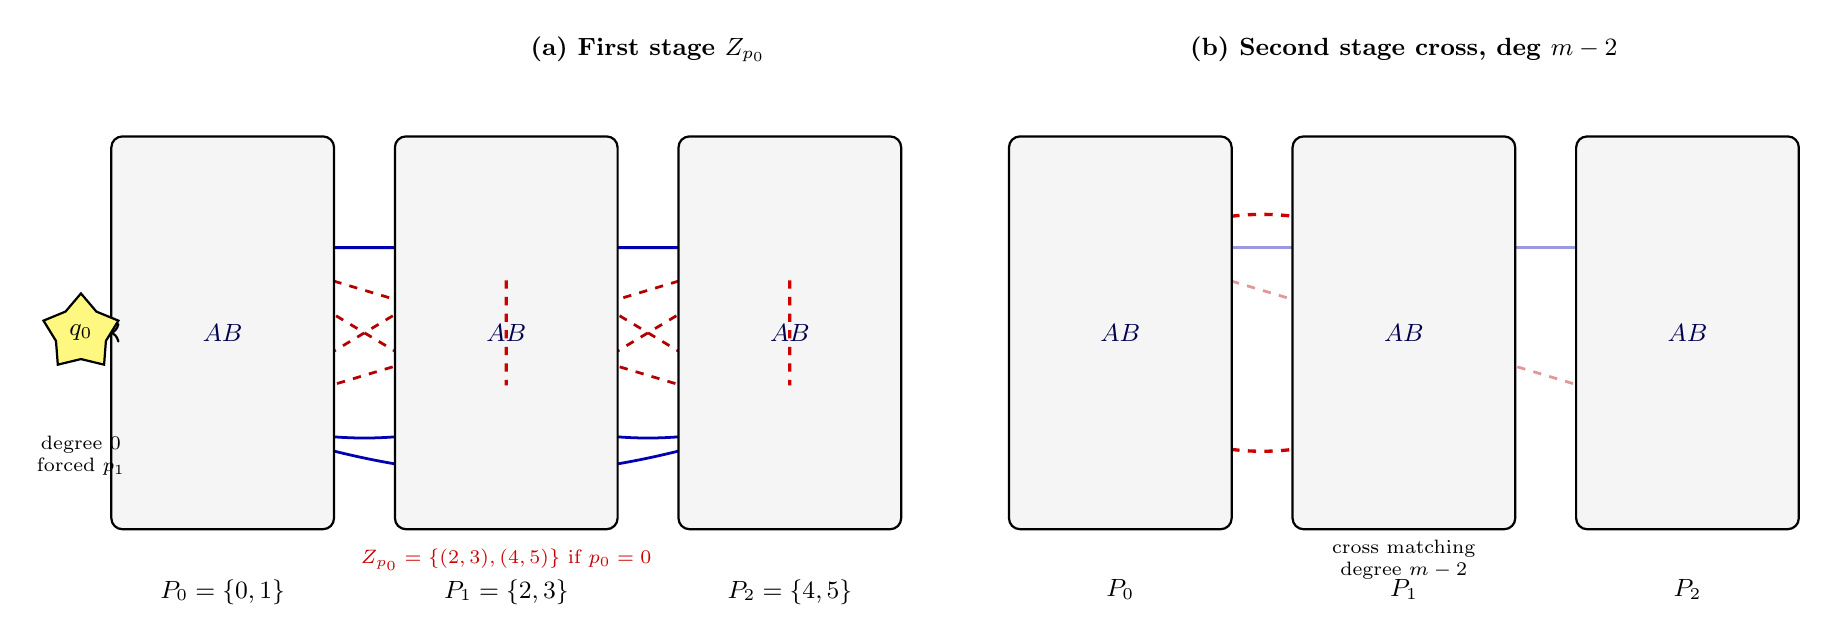
\begin{tikzpicture}[scale=1.2,
  vertex/.style={circle,draw,thick,minimum size=8mm,inner sep=0,fill=white, font=\small},
  pairbox/.style={draw,thick,rounded corners,fill=gray!8,inner sep=10mm},
  Ab/.style={blue!70!black,thick,line width=1pt},
  Bb/.style={red!70!black,thick,dashed,line width=1pt},
  zero/.style={red!80!black,ultra thick,dashed,line width=1.2pt}
]
% --- Subfigure (a) first stage ---
\begin{scope}[xshift=0cm]
\node at (4.5,3.0) {\small\textbf{(a) First stage $Z_{p_0}$}};
% vertices
\node[vertex] (v0) at (0,0.9) {$0$};
\node[vertex] (v1) at (0,-0.9) {$1$};
\node[vertex] (v2) at (3.0,0.9) {$2$};
\node[vertex] (v3) at (3.0,-0.9) {$3$};
\node[vertex] (v4) at (6.0,0.9) {$4$};
\node[vertex] (v5) at (6.0,-0.9) {$5$};
% pair boxes
\node[pairbox,fit=(v0)(v1)] (b0) {};
\node[pairbox,fit=(v2)(v3)] (b1) {};
\node[pairbox,fit=(v4)(v5)] (b2) {};
% labels below boxes, not overlapping AB
\node[below=5mm of b0, font=\small] {$P_0=\{0,1\}$};
\node[below=5mm of b1, font=\small] {$P_1=\{2,3\}$};
\node[below=5mm of b2, font=\small] {$P_2=\{4,5\}$};
% AB centered inside boxes, larger font, 70 black
\node[font=\small, blue!30!black] at (b0.center) {$AB$};
\node[font=\small, blue!30!black] at (b1.center) {$AB$};
\node[font=\small, blue!30!black] at (b2.center) {$AB$};
% q0 star
\node[star,star points=5,draw,thick,fill=yellow!50,minimum size=10mm,inner sep=1pt,font=\small] (qstar) at (-1.5,0) {$q_0$};
\node[font=\scriptsize,align=center] at (-1.5,-1.3) {degree $0$\\forced $p_1$};
\draw[->,thick] (qstar) -- (b0);
% cross edges A even-even solid
\begin{scope}[on background layer]
\draw[Ab] (v0) -- (v2);
\draw[Ab] (v0) -- (v4);
\draw[Ab] (v2) -- (v4);
\draw[Ab] (v1) to[bend right=12] (v3);
\draw[Ab] (v1) to[bend right=18] (v5);
\draw[Ab] (v3) to[bend right=12] (v5);
% B even-odd dashed
\draw[Bb] (v0) -- (v3);
\draw[Bb] (v0) -- (v5);
\draw[Bb] (v2) -- (v1);
\draw[Bb] (v2) -- (v5);
\draw[Bb] (v4) -- (v1);
\draw[Bb] (v4) -- (v3);
\end{scope}
% Zp0 thick red dashed
\draw[zero] (v2) -- (v3);
\draw[zero] (v4) -- (v5);
\node[red!80!black,font=\scriptsize,align=center] at (3.0,-2.4) {$Z_{p_0}=\{(2,3),(4,5)\}$ if $p_0=0$};
\end{scope}

% --- Subfigure (b) second stage cross matching ---
\begin{scope}[xshift=9.5cm]
\node at (3.0,3.0) {\small\textbf{(b) Second stage cross, deg $m-2$}};
\node[vertex] (w0) at (0,0.9) {$0$};
\node[vertex] (w1) at (0,-0.9) {$1$};
\node[vertex] (w2) at (3.0,0.9) {$2$};
\node[vertex] (w3) at (3.0,-0.9) {$3$};
\node[vertex] (w4) at (6.0,0.9) {$4$};
\node[vertex] (w5) at (6.0,-0.9) {$5$};
\node[pairbox,fit=(w0)(w1)] (c0) {};
\node[pairbox,fit=(w2)(w3)] (c1) {};
\node[pairbox,fit=(w4)(w5)] (c2) {};
\node[below=5mm of c0, font=\small] {$P_0$};
\node[below=5mm of c1, font=\small] {$P_1$};
\node[below=5mm of c2, font=\small] {$P_2$};
\node[font=\small, blue!30!black] at (c0.center) {$AB$};
\node[font=\small, blue!30!black] at (c1.center) {$AB$};
\node[font=\small, blue!30!black] at (c2.center) {$AB$};
\begin{scope}[on background layer]
% second stage cross matching degree m-2 =1 for m=3? Actually thick red dashed curved
\draw[zero, red!80!black] (w0) to[bend left=20] (w2);
\draw[zero, red!80!black] (w1) to[bend right=20] (w3);
% remaining A,B edges lighter
\draw[Ab, opacity=0.4] (w0) -- (w4);
\draw[Bb, opacity=0.4] (w0) -- (w5);
\end{scope}
\node[font=\scriptsize,align=center] at (3.0,-2.4) {cross matching\\degree $m-2$};
\end{scope}
\end{tikzpicture}
\end{adjustbox}
\caption[Pairing structure of $M_{2m}$]{Pairing structure of $M_{2m}$ for $m=3$. Pair-boxes $P_k=\{2k,2k+1\}$ carry the within-pair entry $AB$; cross-pair blocks are $\left(\begin{smallmatrix}A&B\\B&A\end{smallmatrix}\right)$. (a) First stage: $Z_{p_0}$ is a perfect matching on the other $m-1$ pairs (degree $m-1$); the partner $q_0$ has degree $0$, forcing $p_1=q_0$. (b) Second stage: the cross matching has degree $m-2\ge1$ for $m\ge3$.}
\label{fig:pairing}
\end{figure}
\end{aiblock}
\begin{humanblock}
\begin{remark}\label{rem:astar-family}
The matrix $A^*$ in Theorem \ref{thm:Astar} has the shape of the $M_{2m}$ family at order four. Normalized to unit diagonal, $|r_{03}|=|r_{12}|=1/4$ and all four cross entries have modulus $1/2$. Hence, after relabeling $(0,3,1,2)$ and conjugating by the diagonal sign matrix $D=\operatorname{diag}(-1,1,1,1)$ --- which preserves positive definiteness and leaves every $t^{(S)}_{jk}=-\log|r^{(S)}_{jk}|$ unchanged, so it preserves the entire cancellation structure --- $A^*$ becomes the matrix $M_4$ of Theorem~\ref{thm:M2m} with $m=2$, $A=B=1/2$, $AB=1/4$. This parameter point is off the curve, since $A^2+(1-B^2)A-1=-3/8\neq0$, but the curve is not what makes $A^*$ fail only the First-Schur Conjecture. For $m=2$ and any $0<A,B<1$ the matrix $M_4$ is positive definite, with eigenvalues $1+AB+A+B$, $(1+A)(1-B)$, $(1-A)(1-B)$ and $(1-A)(1+B)$. Step~1 of the proof of Theorem~\ref{thm:M2m}, which holds for all parameters, shows that every first pivot zeroes the within-pair entry of the other pair, so Conjecture~\ref{conj:2} fails, while Conjecture~\ref{conj:1} holds by Theorem~\ref{thm:leq4}. The curve enters only in step~5, which needs $m\ge3$.
\end{remark}
\end{humanblock}

\section{Consequences for solver authors}\label{sec:practical}
\begin{humanblock}
Two questions a reader implementing sparse Cholesky will ask deserve explicit answers. \emph{Must a
solver test for these cancellations?} No: symbolic factorization allocates for $G^+_\sigma$, and by
Definition~\ref{def:numeric} the numeric pattern is contained in the symbolic one, so a cancellation
can only leave a reserved entry holding an exact zero. The factorization and the solve remain correct,
at the price of a slightly over-allocated structure, and none of our counterexamples makes a standard
code return a wrong answer; a solver that wanted to reclaim that space would have to test numerically
during the factorization, and Theorem~\ref{thm:M2m} shows that no ordering can guarantee those tests
all fail. \emph{Is there a benefit to knowing that a clean ordering exists?} Not for allocation, which
is driven by $G^+_\sigma$ either way, but for diagnosis: an exact zero at a predicted-nonzero position
is an artefact of the ordering when the pattern lies in one of the classes of
Theorem~\ref{thm:positives}, whereas for $K_6$ it may be intrinsic to the matrix
(Theorem~\ref{thm:M2m}). In the statistical reading of Section~\ref{sec:stats} this is the difference
between an unfaithfulness a reordering can remove and one it cannot. We claim no performance
consequence.
\end{humanblock}

\section{Status and open problems}\label{sec:status}
\begin{humanblock}
It is worth collecting in one place what the preceding sections establish and what they leave open,
since a paper that pairs an impossibility result with a list of positive classes makes the two easy to
conflate.

\emph{The existential question is settled, and settled negatively.} Conjecture~\ref{conj:2} already
fails at order four: the matrix $A^*$ of Theorem~\ref{thm:Astar}, with spectrum $\{9,3,3,1\}$, has no
ordering whose first Schur complement is cancellation-free, while $8$ of its $24$ orderings
nevertheless deliver a clean factor. The gap between those two counts is the refill phenomenon, and
isolating it is precisely what allows the stronger Conjecture~\ref{conj:1} to survive at order four.
Conjecture~\ref{conj:1} itself fails at every even order $n\ge6$, by the family $M_{2m}$ of
Theorem~\ref{thm:M2m}, so the smallest known pattern on which cleanliness genuinely fails is the
complete graph $K_6$; whether some pattern of order five fails, $K_5$ in particular, is open.

\emph{The counterexample is derived rather than exhibited.} This is the part of the argument we would
emphasize, because it is what distinguishes the result from a lucky search. We did not find a matrix
and then verify it. The Pairing Lemma~\ref{lem:pairing} classifies the zero-configurations available at
a level with four surviving vertices, and shows that a feasible family of maximal size using all four
survivors as apexes must be a fixed-point-free involution. For counterexamples built this way,
evenness of the order is then a consequence rather than a hypothesis; the magnitudes $AB$ within pairs and the blocks
$\begin{pmatrix}A&B\\B&A\end{pmatrix}$ across them are consequences; and the curve
$A^2+(1-B^2)A-1=0$ is a consequence. By Remark~\ref{rem:curve-family} what emerges at each even order
is a one-parameter family on a measure-zero algebraic curve, not an isolated matrix, and the
inequalities $0<B<A<1$ follow from the equation instead of being imposed alongside it. How far that
rigidity extends is the subject of Question~\ref{q:curve} below.

\emph{The positive side is a boundary rather than a miscellany.} Conjecture~\ref{conj:1} holds for
every pattern of order at most four (Theorem~\ref{thm:leq4}), by an elementary case analysis that uses
only the pivot update, the cancellation graph and four lemmas. Beyond that, Theorem~\ref{thm:forest}
gives forests in the strong form that \emph{every} ordering is clean, which recovers in factorization
language the covariance-faithfulness theorem of Malouche and Rajaratnam~\cite{Malouche}, and
Theorem~\ref{thm:positives} adds $2$-path strips, dominating-vertex fans, chordal graphs with exactly
one triangle, and chordal graphs of clique number at most three whose triangles are pairwise
edge-disjoint. Each of these classes is adaptive of necessity: the triangle lies in all of them, and no single
fixed ordering is clean for every matrix with that pattern (Remark~\ref{rem:no-fixed}), so the
quantifier order in Conjecture~\ref{conj:1} is a feature of the problem and not of its phrasing. All of
these classes have clique number at most three, while the failures we know are complete graphs; where
the boundary lies between the two is open.

\emph{The apparatus is reusable, and is the part most likely to outlast the specific results.}
Cleanliness is recast as a covering problem over slots: a slot $(S,\{j,k\})$ asserts
$(A/A_S)_{jk}=0$, a blocking family is one that meets every ordering, and
Conjecture~\ref{conj:1} fails for a pattern exactly when some blocking family is realizable
(Remark~\ref{rem:covering}). The additive parametrization turns the multiplicative cancellation
condition into a linear system, infeasibility of which is certified by an integer Stiemke witness, and
the pattern-level lemmas --- Prefix, fresh-fill closure, zero-leg, Nesting, Exchange and Monotone ---
are what make families refutable without reference to any particular matrix.

\emph{No theorem in this paper depends on a computation.} Every result above is proved by hand, in
exact arithmetic where arithmetic is needed at all. The ancillary scripts of
Appendix~\ref{app:protocol} recompute asserted values independently, and
Appendix~\ref{app:recheck} is explicit that both the order-four slot search and the four-vertex
feasibility counts corroborate rather than constitute the proofs they accompany. The computations
reported in Remark~\ref{rem:even-needed} and the order-five search below concern cases that remain
open, and together with the sampling count of Remark~\ref{rem:peo-fail} they are the places where
this reading needs care: they are not steps in any argument, nothing established above depends on
them, and the order-five and order-seven searches and that sampling run are not included in the
ancillary material.

\emph{What is not settled.} The overall shape of the results is that the positive side is governed by
the scarcity of triangles and by the availability of a simplicial or universal pivot, whereas the
negative side, so far, uses complete patterns. Three frontiers remain open --- order five, the
connected patterns of order six other than $K_6$, and all odd orders from seven upwards. The first two are finite
questions that we leave undecided; the third is not, and Remark~\ref{rem:even-needed} explains why the
parity argument that settles the even orders gives nothing there. To these we add the structural
question of how much the even-order construction really forces.

\emph{How far order five has been pushed.} The order-five question is finite, and we have gone some way into it without settling it. Using the covering reformulation of Remark~\ref{rem:covering} together with the pattern rules of Section~\ref{sec:core}, a depth-first search over partial blocking families closes twenty of the twenty-one connected patterns of order five: for each of them every branch ends in a refutation, by a pattern rule or, where the rules do not suffice, by an integer Stiemke certificate checked in exact arithmetic. The complete graph $K_5$  is the exception. There the search does not terminate, with branches reaching families of some twenty slots without closing, and the natural alternative — enumerating the minimal blocking families of $K_5$ and refuting each — is worse, since a direct enumeration passes $2\times 10^7$   of them without exhausting the list. Because the order-five statement would rest on a single unresolved pattern, we record this as an observation rather than a theorem. The search is not included in the ancillary material.

%\subsection{Open}
Six questions are left open: order five; the connected patterns of order six other than $K_6$, of which
$K_6-e$ is the densest; all odd orders $n\ge7$; general partial $2$-trees; outerplanar graphs in general; and whether the $M_{2m}$
curve accounts for every even-order counterexample. Two of them we state formally: the rigidity
question just mentioned, and a scheduling question which arose while proving
Theorem~\ref{thm:positives}(i) and which would extend it.

\begin{question}[Does the curve exhaust the even-order counterexamples?]\label{q:curve}
Is every counterexample to Conjecture~\ref{conj:1} at even order $n\ge6$ a point of the $M_{2m}$ curve
\eqref{eq:curve}, up to permutation and diagonal scaling?
\end{question}

Theorem~\ref{thm:M2m} gives no information here, because it is existential: it produces
counterexamples and shows that their parameters are forced once the pairing shape is assumed, but it
never quantifies over all SPD matrices of a given order. The forcing in Lemma~\ref{lem:pairing} is
conditional in the same way. It applies to a level with exactly four survivors carrying a feasible
family of maximal size that uses all four of them as apexes, and only three of the fifteen maximal
feasible families at such a level meet that last condition; at five survivors the classification fails
outright, since feasible families using all five apexes exist there
(Remark~\ref{rem:even-needed}). A counterexample resting on a different mechanism is therefore not
excluded by anything we prove, and we state Question~\ref{q:curve} as a question rather than as a
conjecture because we have no evidence either way.

An affirmative answer would be strong, and the reason is worth recording. Every off-diagonal entry of
$M_{2m}$ is nonzero, and permutation and diagonal scaling preserve this, so every counterexample on the
curve has a complete pattern. An affirmative answer at $n=6$ would therefore show that every connected
pattern of order six other than $K_6$ admits a clean ordering for every SPD matrix of that pattern,
settling order six, one of the two finite frontiers above. Question~\ref{q:curve} is in that sense at
least as hard as the whole of order six, and a counterexample to it would be at least as interesting as a proof: it would mean
that the mechanism isolated by the Pairing Lemma is not the only route to failure.

\begin{question}[Clean strategies ending at a prescribed edge]\label{q:cliquesum}
Does every $2$-path strip, and every dominating-vertex fan, admit an adaptive clean strategy whose
last two pivots are the two ends of a prescribed boundary edge?
\end{question}

An affirmative answer would give Conjecture~1 for clique sums along cliques of size at most two, and
hence for strips and fans glued along an edge or a vertex.\footnote{%
Sketch. Let $G=G_1\cup G_2$ with $G_1\cap G_2=K$ a clique, $|K|\le2$; suppose $G_2$ admits an adaptive
clean strategy~(a) eliminating $K$ last, and $G_1$ an adaptive clean strategy~(b). Pivot
$G_2\setminus K$ by the initial segment of~(a), then $G_1\cup K$ by~(b). Since no vertex of $K$ is
pivoted in phase~1, no pair inside $K$ is committed there, and because $K$ separates, $A[G_2]$ is a
principal submatrix with pattern $G_2$ on which phase~1 is exactly~(a); as $K$ comes last in~(a), the
pair inside $K$ is still nonzero after phase~1. By the fill-path theorem no fill crosses the
separator, so the Schur complement handed to phase~2 is $A[G_1]$ altered only in the $K\times K$ block
and still has pattern $G_1$; since~(b) is adaptive it is valid for every SPD matrix of that pattern,
so phase~2 is clean. Only hypothesis~(a) is at issue, and it is exactly
Question~\ref{q:cliquesum}.}
The obstruction is the final triangle. Running the strip induction from the left end leaves
$\{v_{k-2},v_{k-1},v_k\}$ as the last three survivors, and Lemma~\ref{lem:tri} supplies only
\emph{some} clean apex among them; finishing with $K=\{v_{k-1},v_k\}$ requires the apex to be
$v_{k-2}$. If $v_{k-2}$ is the dirty vertex of that triangle, pivoting it commits a zero at the
$K$-pair. No refill argument repairs this, because refill (Lemma~\ref{lem:fact1}) needs the zero to
pre-exist the pivot that destroys it, whereas here the offending pivot is itself the apex that creates
it; and reversing the direction of the induction merely relocates the final triangle. A positive
answer would also bear on the question of outerplanar graphs in the list above.
\end{humanblock}
% \subsection{Mathematical retractions}
% \begin{enumerate}
% \item Withdrawn: claim that condition for cancellation $A_{ij}=A_{vi}A_{vj}/a_v$ characterizing badness holds at all stages, not just first stage — false, first stage only. This corresponds to earlier $R2^*$ generalisation attempt.
% \item Withdrawn: claim that any sparse pattern can be made dense $K_n$ via $\epsilon$-perturbation preserving cancellations — flawed proof, earlier $K_n$ approximation lemma.
% \item Minimal separator size $\le2$ bounds treewidth -- false due to $K_n$ vacuous zero separators. Witness $K_n$ has zero minimal separators.
% \item Jacobi cleanliness duality: $\det$ identity survives, corollary $\sigma$ clean for $A$ iff $\operatorname{rev}(\sigma)$ clean for $A^{-1}$ false. Witness $A=\begin{pmatrix}2&1&0\\1&3&1\\0&1&2\end{pmatrix}$, $\det8$, path pattern $(0,2,1)$ clean yet $(A^{-1}/A^{-1}_{11})_{02}=1/8-1/8=0$ at position predicted nonzero because $A^{-1}$ dense.
% \item Every partially eliminated pattern chordal -- false. $M=\begin{pmatrix}4&0&1&1\\0&4&1&1\\1&1&4&0\\1&1&0&4\end{pmatrix}$, $B=\begin{pmatrix}1&v^\top\\v&M+vv^\top\end{pmatrix}$: $B$ dense SPD symbolic fill complete chordal but $B/B_{00}=M$ chordless 4-cycle.
% \item Outerplanar follows from fans -- unproved, open.
% \end{enumerate}

\section{Conclusion}
\begin{humanblock}
The existential question has a negative answer in general and a positive one on a class we can now
delimit. Conjecture~\ref{conj:2} is false already at order four (Theorem~\ref{thm:Astar}): the matrix
$A^*$ admits no ordering whose first Schur complement is cancellation-free, yet $8$ of its $24$
orderings still yield a clean factor, which is the refill phenomenon in its simplest form.
Conjecture~\ref{conj:1} holds for $n\le4$ by an elementary case analysis with no computation
(Theorem~\ref{thm:leq4}), and fails at every even order $n\ge6$ through the family $M_{2m}$
(Theorem~\ref{thm:M2m}). That family is derived rather than exhibited: classifying the
zero-configurations available at a level with four surviving vertices forces a fixed-point-free
involution, hence even order, and forces the magnitudes within and across pairs, so the curve
$A^2+(1-B^2)A-1=0$ on which this family lies is imposed by the classification rather than chosen. The
forcing is a rigidity statement about counterexamples of this shape; it does not assert that every
counterexample lies on the curve (Question~\ref{q:curve}). Every point of that curve with $0<B<1$
yields a counterexample, and $B=1/2$ is the instance we
verify explicitly.

On the positive side, forests are clean in the strong sense that every ordering is clean
(Theorem~\ref{thm:forest}), and Conjecture~\ref{conj:1} also holds for $2$-path strips, for
dominating-vertex fans, for chordal graphs with exactly one triangle, and for chordal graphs of
clique number at most three whose triangles are pairwise edge-disjoint (Theorem~\ref{thm:positives});
on each class of Theorem~\ref{thm:positives} the clean ordering must adapt to the matrix, since no
fixed ordering suffices even for the triangle (Remark~\ref{rem:no-fixed}).

Two gaps remain, and they are of different kinds. Order five we leave open: the question there is
finite, pattern by pattern, but we do not settle it. Odd orders $n\ge7$ are open for a structural
reason rather than a computational one, since the pairing classification that drives the even
construction requires exactly four survivors and its injectivity step fails at five
(Remark~\ref{rem:even-needed}); the square-count identity is evidence about where counterexamples
could live rather than an obstruction to their existence, because the counterexamples we construct lie
on a singular locus that such counting does not detect.

For practice the conclusion is reassuring in the direction that matters. The no-cancellation assumption
of symbolic factorization remains safe for allocation, since over-allocation never threatens
correctness, and none of our counterexamples causes a standard code to return a wrong answer. What is
not guaranteed is the existential statement: at every even order from six upwards there are SPD matrices for which no
ordering avoids an exact zero at a position the symbolic phase predicts nonzero. The ancillary
scripts listed in Appendix~\ref{app:protocol} reproduce the numerical claims they cover, and
Appendix~\ref{app:recheck} reports the independent recomputation and says which computations are not
included.
\end{humanblock}

\section*{Acknowledgments}

The author would like to thank Ricky Simanjuntak for discussions at various stages of this project and his feedback on the final draft. The authors would also like to thank Paul Bendich and Patrick Tam for so kindly reviewing this work and offering very thoughtful suggestions and edits which have greatly improved the content of this draft. 


\appendix
\section{Computational protocol}\label{app:protocol}
\begin{humanblock}
All computations reported here were carried out in Python~$3.11.9$. The ancillary scripts need only
the standard library, with exact integer or rational arithmetic, except \texttt{enum-pairing-4vert.py},
which uses NumPy and SciPy's \texttt{linprog} (its counts are reproduced without a solver by
\texttt{slot\_counts.py}). Pseudorandom draws, which enter only the sampling
experiment of Appendix~\ref{app:recheck}, were seeded with $42$, $123$ and $2026$. Where a linear program is solved --- in the order-four slot search of
Appendix~\ref{app:recheck} and in the feasibility counts reported there --- HiGHS~\cite{HiGHS} serves
only as a search device for a candidate certificate, and correctness never rests on it. By Stiemke's
alternative, infeasibility of $Tt=0$, $t>0$ is witnessed by an integer vector $y$ with
$y^\top T\ge0$ and $y^\top T\neq0$; since $T$ has integer entries such a witness is checked by integer
arithmetic alone, so no floating-point computation enters any proof.

Six scripts are provided as ancillary files. \texttt{verify\_cholesky.py} recomputes the worked
instances of Theorems~\ref{thm:Astar} and~\ref{thm:M2m} from their statements alone.
\texttt{enum-pairing-4vert.py} enumerates the $2^{12}=4096$ slot subsets at a four-vertex level and
finds $182$ of them feasible, the computation behind the three all-pivot configurations of
Lemma~\ref{lem:pairing}. \texttt{three-mag-59049.py} sweeps the $3^{10}=59049$ three-magnitude
colourings at order five, establishing the minimum survivor count of $8$ reported in
Remark~\ref{rem:even-needed}. \texttt{peo\_insufficiency.py} runs all $5040$ orderings of an SPD
realization of the $2$-path of $5$ triangles, the witness of Remark~\ref{rem:peo-fail}.
\texttt{fixed\_ordering\_witnesses.py} checks the witnesses of Remark~\ref{rem:no-fixed}: the three
realizations of the triangle and the five realizations of the pattern $E$ defeat every fixed
ordering. \texttt{slot\_counts.py} decides feasibility exactly, by Fourier--Motzkin elimination in
rational arithmetic, and reproduces the four-vertex counts of Lemma~\ref{lem:pairing}, the order-four
slot search of Appendix~\ref{app:recheck}, and the order-five slot bounds of
Remark~\ref{rem:even-needed}. For the
instance of Theorem~\ref{thm:M2m} used throughout, $B=1/2$ and
$A=(-3+\sqrt{73})/8$, so that $B(1-A)=11/16-\sqrt{73}/16\approx0.1534997659$.
\end{humanblock}

\section{Source of \texttt{verify\_cholesky.py}}\label{app:code}
\mbox{}

% The listing is split into page-sized pieces so that each one fits inside a single
% aiblock; firstnumber keeps the printed line numbering continuous across the pieces.
% Ranges refer to lines of verify_cholesky.py (569 lines total).

\begin{aiblock}
\mbox{}
\lstinputlisting[style=pycode, firstline=1, lastline=58, firstnumber=1]{\ancillary{Appendix_VerifyCholesky/verify_cholesky.py}}
\end{aiblock}

\begin{aiblock}
\mbox{}
\lstinputlisting[style=pycode, firstline=59, lastline=111, firstnumber=59]{\ancillary{Appendix_VerifyCholesky/verify_cholesky.py}}
\end{aiblock}

\begin{aiblock}
\mbox{}
\lstinputlisting[style=pycode, firstline=112, lastline=170, firstnumber=112]{\ancillary{Appendix_VerifyCholesky/verify_cholesky.py}}
\end{aiblock}

\begin{aiblock}
\mbox{}
\lstinputlisting[style=pycode, firstline=171, lastline=219, firstnumber=171]{\ancillary{Appendix_VerifyCholesky/verify_cholesky.py}}
\end{aiblock}

\begin{aiblock}
\mbox{}
\lstinputlisting[style=pycode, firstline=220, lastline=275, firstnumber=220]{\ancillary{Appendix_VerifyCholesky/verify_cholesky.py}}
\end{aiblock}

\begin{aiblock}
\mbox{}
\lstinputlisting[style=pycode, firstline=276, lastline=330, firstnumber=276]{\ancillary{Appendix_VerifyCholesky/verify_cholesky.py}}
\end{aiblock}

\begin{aiblock}
\mbox{}
\lstinputlisting[style=pycode, firstline=331, lastline=389, firstnumber=331]{\ancillary{Appendix_VerifyCholesky/verify_cholesky.py}}
\end{aiblock}

\begin{aiblock}
\mbox{}
\lstinputlisting[style=pycode, firstline=390, lastline=434, firstnumber=390]{\ancillary{Appendix_VerifyCholesky/verify_cholesky.py}}
\end{aiblock}

\begin{aiblock}
\mbox{}
\lstinputlisting[style=pycode, firstline=435, lastline=490, firstnumber=435]{\ancillary{Appendix_VerifyCholesky/verify_cholesky.py}}
\end{aiblock}

\begin{aiblock}
\mbox{}
\lstinputlisting[style=pycode, firstline=491, lastline=534, firstnumber=491]{\ancillary{Appendix_VerifyCholesky/verify_cholesky.py}}
\end{aiblock}

\begin{aiblock}
\mbox{}
\lstinputlisting[style=pycode, firstline=535, lastline=569, firstnumber=535]{\ancillary{Appendix_VerifyCholesky/verify_cholesky.py}}
\end{aiblock}


\section{Source of \texttt{enum-pairing-4vert.py}}\label{app:code-pairing}
\mbox{}

% Split so each piece fits inside one aiblock; firstnumber keeps the numbering
% continuous. Ranges refer to lines of enum-pairing-4vert.py (83 lines total).

\begin{aiblock}
\mbox{}
\lstinputlisting[style=pycode, firstline=1, lastline=46, firstnumber=1]{\ancillary{Appendix_EnumPairing4Vert/enum-pairing-4vert.py}}
\end{aiblock}

\begin{aiblock}
\mbox{}
\lstinputlisting[style=pycode, firstline=47, lastline=83, firstnumber=47]{\ancillary{Appendix_EnumPairing4Vert/enum-pairing-4vert.py}}
\end{aiblock}

\section{Source of \texttt{three-mag-59049.py}}\label{app:code-threemag}
\mbox{}

% The whole script (61 lines) fits inside one aiblock.

\begin{aiblock}
\mbox{}
\lstinputlisting[style=pycode, firstline=1, lastline=61, firstnumber=1]{\ancillary{Appendix_ThreeMag59049/three-mag-59049.py}}
\end{aiblock}

\section{Source of \texttt{peo\_insufficiency.py}}\label{app:code-peo}
\mbox{}

% Split so each piece fits inside one aiblock; firstnumber keeps the numbering
% continuous. Ranges refer to lines of peo_insufficiency.py (90 lines total).

\begin{aiblock}
\mbox{}
\lstinputlisting[style=pycode, firstline=1, lastline=43, firstnumber=1]{\ancillary{Appendix_PeoInsufficiency/peo_insufficiency.py}}
\end{aiblock}

\begin{aiblock}
\mbox{}
\lstinputlisting[style=pycode, firstline=44, lastline=90, firstnumber=44]{\ancillary{Appendix_PeoInsufficiency/peo_insufficiency.py}}
\end{aiblock}

\section{Source of \texttt{fixed\_ordering\_witnesses.py}}\label{app:code-fixed}
\mbox{}

% Split so each piece fits inside one aiblock; firstnumber keeps the numbering
% continuous. Ranges refer to lines of fixed_ordering_witnesses.py (143 lines total).

\begin{aiblock}
\mbox{}
\lstinputlisting[style=pycode, firstline=1, lastline=50, firstnumber=1]{\ancillary{Appendix_FixedOrderingWitnesses/fixed_ordering_witnesses.py}}
\end{aiblock}

\begin{aiblock}
\mbox{}
\lstinputlisting[style=pycode, firstline=51, lastline=114, firstnumber=51]{\ancillary{Appendix_FixedOrderingWitnesses/fixed_ordering_witnesses.py}}
\end{aiblock}

\begin{aiblock}
\mbox{}
\lstinputlisting[style=pycode, firstline=115, lastline=143, firstnumber=115]{\ancillary{Appendix_FixedOrderingWitnesses/fixed_ordering_witnesses.py}}
\end{aiblock}


\section{Source of \texttt{slot\_counts.py}}\label{app:code-slots}
\mbox{}

% Split so each piece fits inside one aiblock; firstnumber keeps the numbering
% continuous. Ranges refer to lines of slot_counts.py (120 lines total).

\begin{aiblock}
\mbox{}
\lstinputlisting[style=pycode, firstline=1, lastline=28, firstnumber=1]{\ancillary{Appendix_SlotCounts/slot_counts.py}}
\end{aiblock}

\begin{aiblock}
\mbox{}
\lstinputlisting[style=pycode, firstline=29, lastline=120, firstnumber=29]{\ancillary{Appendix_SlotCounts/slot_counts.py}}
\end{aiblock}


\section{Independent recomputation of the numerical claims}\label{app:recheck}
\begin{humanblock}
The numerical and combinatorial assertions listed below have been recomputed
independently, in exact arithmetic, by an implementation written from the
statements alone (no shared code with the primary verification of
Appendix~\ref{app:protocol}). Rational quantities were handled with exact
rationals; the irrational parameter was handled by exact arithmetic in the
quadratic field $\mathbb{Q}(\sqrt{73})$, representing every quantity as
$p+q\sqrt{73}$ with $p,q\in\mathbb{Q}$, so that all zero tests are exact and no
floating-point tolerance is used.

The recomputation covers the spectrum and positive definiteness of $A^*$ and of $M_{2m}$ for
$m=2,3,4$, the two parameter identities and the vanishing of $A^2+(1-B^2)A-1$ at
$A=(-3+\sqrt{73})/8$, the clean-ordering counts $0/24$ and $8/24$ for $A^*$ and $0/720$ and $0/40320$
for $M_6$ and $M_8$, the pairing classification of Lemma~\ref{lem:pairing}, and the square-count identity
$n\lceil(n-2)/2\rceil=\binom{n}{2}$ for odd $n$ in the range $3\le n\le11$. Every asserted value was
reproduced exactly. One quantity emerged from the recomputation that the text uses only in the
discussion of Question~\ref{q:curve}: there are
$15$ feasible slot sets of the maximum size $4$ at a four-vertex level, of which only $3$ use all four
pivots, which is why Lemma~\ref{lem:pairing} has to impose the all-four-pivots condition explicitly.
The recomputation also separates the two necessary conditions of that lemma from feasibility
itself: $218$ of the $4096$ subsets have an acyclic arc digraph, so the General Cycle
Lemma~\ref{lem:cycle} leaves $36$ infeasible subsets undetected, and the feasible count $182$ is a
linear-programming count rather than a cycle count. None of these counts is used in
the proof of Lemma~\ref{lem:pairing}, which is elementary; they are recorded here as
corroboration and as context for the size bound that the lemma does prove. This recomputation is
not included in the ancillary material; \texttt{slot\_counts.py} (Appendix~\ref{app:code-slots})
reproduces the counts $182$, $15$ and $3$ in exact arithmetic.

It is worth recording why random search does not find the counterexamples of
Section~\ref{sec:even}. Adversarial sampling on dense $K_6$, in which the entries of a random SPD matrix are
perturbed towards the cancellation conditions, bottoms out near $296/720$ clean orderings in our runs
and never approaches the $0/720$ of $M_6$, because $M_6$ lies on the measure-zero curve $A^2+(1-B^2)A-1=0$. We report this as an
indication of the difficulty rather than as evidence: the perturbation scheme and the number of draws
are implementation choices, and no claim in this paper depends on them. These runs are not
included in the ancillary material. This is the coexistence noted
in Section~\ref{sec:stats}: unfaithful distributions form a null set while strong-faithfulness fails on
a set of positive measure \cite{Uhler}, so the genericity heuristic and the existential failure are
consistent with one another.

An exhaustive slot search at order four was also carried out, over the $18$ slots with
$1\le|S|\le2$ on $G_A=K_4$: of the $2^{18}=262144$ slot families, $69075$ are blocking and $633$
of these are minimal, and all $633$ are refuted by exact rational certificates ($605$ by Stiemke's
lemma, $28$ by zero-leg propagation). The script \texttt{slot\_counts.py} reproduces the counts $69075$
and $633$; the certificates are not included in the ancillary material. This corroborates Theorem~\ref{thm:leq4} but is no longer
part of its proof, which is elementary.
\end{humanblock}

\bibliographystyle{alpha}
\bibliography{bib}
\end{document}

